\documentclass[german]{spicker}

%\addbibresource{num1.bib}

\title{Numerik 1}
\author{Patrick Gustav Blaneck}
\makeindex[intoc]
\makeindex[intoc, name=Beispiele,title=Beispiele]

\begin{document}
\maketitle
\tableofcontents
\newpage

\section{Einleitung}

\begin{defi}{Numerik}
    Lloyd Trefethen 1992:
    \begin{displayquote}
        Numerical analysis is the study of algorithms for the problems of continuous mathematics.
    \end{displayquote}

    \enquote{continuous mathematics} heißt, dass reelle oder komplexe Zahlen beteiligt sind, in Abgrenzung zur diskreten Mathematik.
    Dies umfasst die Analysis und Teile der linearen Algebra.

    Die \emph{Numerik} beschäftigt sich mit der Entwicklung von (effizienten) Berechnungsmethoden, da viele mathematische Objekte zwar wohldefiniert sind, aber nicht endlich berechenbar.
\end{defi}

\begin{example}{Auswertung der Exponentialfunktion}
    Zu berechnen sei $e^{\frac{1}{2}}$, wie Exponentialfunktion bekanntermaßen wie folgt definiert ist:
    \[
        e^x = \sum_{k=0}^\infty \frac{x^k}{k!}
    \]

    Die unendliche Summe ist nicht direkt berechenbar, daher wird ein Ersatzproblem gelöst:
    \[
        e^x \approx \sum_{k=0}^n \frac{x^k}{k!}
    \]
    Dabei ist $n$ ein neuer freier Parameter.
    Es gilt:
    \begin{itemize}
        \item kleines $n$ $\implies$ eventuell zu viel vernachlässigt, Wert ungenau approximiert.
        \item großes $n$ $\implies$ Berechnung aufwändig, Gewinn an Genauigkeit potentiell gering.
    \end{itemize}

    Ein weiteres Problem kann durch eine nicht-exakte Arithmetik aufkommen.
    Seien die beiden Summationsreihenfolgen $s_1(x)$ und $s_2(x)$ gegeben:
    \[
        s_1(x) = 1 + x + \frac{x^2}{2} + \ldots + \frac{x^n}{n!}
    \]
    \[
        s_2(x) = \frac{x^n}{n!} + \ldots + \frac{x^2}{2} + x + 1
    \]

    Bei einer Floating-Point-Rechnung mit 3 Stellen Genauigkeit gilt:
    \begin{center}
        \begin{tabular}{|C||C|C|C|C|C|}
            \hline
            n        & 1   & 2    & 3    & 4    & 5    \\
            \hline
            \hline
            s_1(0.5) & 1.5 & 1.62 & 1.64 & 1.64 & 1.64 \\
            \hline
            s_2(0.5) & 1.5 & 1.62 & 1.65 & 1.65 & 1.65 \\
            \hline
        \end{tabular}
    \end{center}

    Die Summationsreihenfolge beeinflusst also das Ergebnis.

    Ein Abbruch bei $n=4$ ist für $x = \nicefrac{1}{2}$ angemessen.
\end{example}


\begin{example}{Rechteckregel und Trapezregel}
    Zu approximieren sei die Funktion
    \[
        f(x) = \int_{0}^{1} \frac{1}{1+x^2} \diff x
    \]

    \emph{Rechteckregel} und \emph{Trapezregel} approximieren diese Funktion wie folgt:

    % Rechteckregel
    \begin{tikzpicture}
        \begin{axis}[
                axis lines = left,
                %xlabel = $x$,
                %ylabel = $f(x)$,
                xmin = 0,
                xmax = 1.05,
                ymin = 0,
                ymax = 1.05,
            ]

            \addplot[name path=f,domain = 0:1.05,samples = 100] { 1/(1+x^2) };

            \addplot[dashed] coordinates{(1,0) (1,1)};

            \path[name path=axis] (axis cs:0,0) -- (axis cs:1,0);
            \path[name path=approx] (axis cs:0,1) -- (axis cs:1,1);

            \addplot[fill=red,fill opacity=0.1] fill between[of=approx and axis,soft clip={domain=0:1}];
        \end{axis}
    \end{tikzpicture}
    % Trapezregel
    \begin{tikzpicture}
        \begin{axis}[
                axis lines = left,
                %xlabel = $x$,
                %ylabel = $f(x)$,
                xmin = 0,
                xmax = 1.05,
                ymin = 0,
                ymax = 1.05,
            ]

            \addplot[name path=f,domain = 0:1.05,samples = 100] { 1/(1+x^2) };

            \addplot[dashed] coordinates{(1,0) (1,1)};

            \path[name path=axis] (axis cs:0,0) -- (axis cs:1,0);
            \path[name path=approx] (axis cs:0,1) -- (axis cs:1,0.5);

            \addplot[fill=blue,fill opacity=0.1] fill between[of=approx and axis,soft clip={domain=0:1}];
        \end{axis}
    \end{tikzpicture}

    TO DO
\end{example}

\begin{defi}{Numerische Simulation}
    \emph{Numerische Simulation} beschreibt die Verhaltensvorhersage eines physikalischen Systems durch mathematische Modelle und numerische Verfahren.

    Numerische Simulationen sind z.B. anwendbar in physikalischen Systemen (beliebige Bauteile) und daher sehr wichtig für die Produktentwicklung in der Industrie.

    Das Vorgehen ist wie folgt:
    \begin{itemize}
        \item virtueller Prototyp: vollständige Analyse durch numerische Simulation
        \item davon ausgehend: endgültige Auslegung der Konstruktion
        \item am Ende: Validierung durch einen realen Prototypen
    \end{itemize}

    In der Regel spart numerische Simulation Geld und Zeit.
\end{defi}
\section{Lineare Gleichungssysteme - Direkte Löser I}

\subsection{Einleitung}

\begin{defi}{Lineares Gleichungssystem}
    Betrachten wir allgemein ein System von $m$ Gleichungen für $n$ Unbekannte, so erhalten wir:
    \[
        \begin{matrix}
            a_{11}x_1 & + & a_{12}x_2 & + & \cdots & + & a_{1n}x_n & = & b_1    \\
            a_{21}x_1 & + & a_{22}x_2 & + & \cdots & + & a_{2n}x_n & = & b_2    \\
            \vdots    &   &           &   &        &   &           &   & \vdots \\
            a_{m1}x_1 & + & a_{m2}x_2 & + & \cdots & + & a_{mn}x_n & = & b_m
        \end{matrix}
    \]
    Es gilt:
    \begin{itemize}
        \item Unbekannte dürfen nur linear auftreten,
        \item $a_{ij} \in \R$ gegebene Koeffizienten,
        \item $b_i \in \R$ gegebene rechte Seite,
        \item $x_j \in \R$ gesuchte Unbekannte
    \end{itemize}

    Zur Abkürzung benutzt man die Matrix-Vektor-Schreibweise
    \[
        Ax = b
    \]
    mit Systemmatrix
    \[
        A =
        \begin{pmatrix}
            a_{11} & \cdots & a_{1n} \\
            \vdots &        & \vdots \\
            a_{m1} & \cdots & a_{mn}
        \end{pmatrix}
        \in \R^{m \times n},
    \]
    rechter Seite
    \[
        b =
        \begin{pmatrix}
            b_1    \\
            \vdots \\
            b_m
        \end{pmatrix}
        \in \R^{m},
    \]
    Vektor der Unbekannten
    \[
        x =
        \begin{pmatrix}
            x_1    \\
            \vdots \\
            x_n
        \end{pmatrix}
        \in \R^{n}
    \]
    und Matrix-Vektor-Produkt
    \[
        Ax =
        \begin{pmatrix}
            a_{11} & \cdots & a_{1n} \\
            \vdots &        & \vdots \\
            a_{m1} & \cdots & a_{mn}
        \end{pmatrix}
        \begin{pmatrix}
            x_1    \\
            \vdots \\
            x_n
        \end{pmatrix}
        =
        \begin{pmatrix}
            a_{11}x_1 & + & a_{12}x_2 & + & \cdots & + & a_{1n}x_n \\
            \vdots    &   &           &   &        &   & \vdots    \\
            a_{m1}x_1 & + & a_{m2}x_2 & + & \cdots & + & a_{mn}x_n
        \end{pmatrix}
    \]
\end{defi}

\begin{bonus}{Lösbarkeit von linearen Gleichungssystemen}
    Sei ein lineares Gleichungssystem mit $A \in \R^{m \times n}$, $b \in \R^{m}$ und $x \in \R^{n}$ gegeben.

    Dann gilt:
    \begin{itemize}
        \item $m \neq n$ $\implies$ (in der Regel) entweder keine Lösung oder unendlich viele,
        \item $m = n$ $\implies$ eindeutig lösbar, falls $A$ regulär\footnote{$A \in \R^{n\times n}$ heißt \emph{regulär}, falls $\det(A) \neq 0$ bzw. \emph{singulär}, falls $\det(A) = 0$.} ist.
    \end{itemize}
\end{bonus}

\begin{bonus}{Wiederholung Matrizen}
    Es gilt:
    \begin{itemize}
        \item $\det(A) \neq 0$ $\iff$ Spalten $s_j = \begin{pmatrix} a_{1j} \\ \vdots \\ a_{nj} \end{pmatrix}$, $j = 1, \ldots, n$ sind linear unabhängig.
        \item $\det(A) \neq 0$ $\iff$ Zeilen $z_i = \begin{pmatrix} a_{i1} & \cdots & a_{in} \end{pmatrix}$, $i = 1, \ldots, n$ sind linear unabhängig.
        \item $A \in \R^{n \times n}$ regulär $\iff$ $\rang(A) = n$
        \item $A \in \R^{n \times n}$ singulär $\iff$ $\rang(A) < n$
        \item $A \in \R^{m \times n}$ definiert eine lineare Abbildung $\R^n \to \R^m$ durch $x \to Ax$.
        \item Jede lineare Abbildung $\R^n \to \R^m$ ist als Matrix darstellbar.
        \item Matrizenmultiplikation ist nur bei passender Dimension möglich.
        \item In der Regel ist Matrizenmultiplikation nicht kommutativ (also $AB \neq BA$).
        \item $(AB)^T = B^TA^T$
        \item $A, B \in \R^{n \times n} \implies \det(AB) = \det(A) \det(B) \implies$ sind $A$, $B$ regulär, dann auch $AB$
        \item Ist $A \in \R^{n \times n}$ regulär, so existiert die Inverse $A^{-1} \in \R^{n \times n}$ mit
              \[
                  A^{-1}A = AA^{-1} = I =
                  \begin{pmatrix}
                      1 &        &   \\
                        & \ddots &   \\
                        &        & 1
                  \end{pmatrix}
              \]
        \item für $A, B$ regulär ist $(AB)^{-1} = B^{-1}A^{-1}$
    \end{itemize}
\end{bonus}

\begin{defi}{Matrixnorm}
    Ist $\norm{\cdot}$ eine Norm auf $\R^n$, $A \in \R^{n \times n}$, dann definiert
    \[
        \norm{A} := \sup_{x \neq 0} \frac{\norm{Ax}}{\norm{x}} = \max_{\norm{x} = 1} \norm{Ax}
    \]
    eine \emph{Matrixnorm} auf $\R^{n \times n}$.

    Eine Matrixnorm erfüllt analog zur Vektornorm die folgenden Bedingungen:
    \begin{enumerate}
        \item $\norm{A} = 0 \iff x = 0$ (Definitheit)
        \item $\norm{\alpha A} = \alpha \norm{A} \quad \forall A \in \R^{n \times n}, \forall \alpha \in \R$ (absolute Homogenität)
        \item $\norm{A + B} \leq \norm{A} + \norm{B} \quad \forall A, B \in \R^{n \times n}$ (Subadditivität oder Dreiecksungleichung)
    \end{enumerate}

    Eine Matrixnorm hängt von der benutzten Vektornorm ab und heißt deshalb die von der Vektornorm \emph{induzierte Matrixnorm}.

    Eine Vektornorm und die induzierte Matrixnorm sind kompatibel, d.h.
    \[
        \norm{Ax} \leq \norm{A} \norm{x}
    \]

    Für induzierte Matrixnormen gilt
    \[
        \norm{AB} \leq \norm{A} \norm{B}
    \]

    Auf $\R^{n \times n}$ sind alle Matrixnormen äquivalent.
\end{defi}

\begin{defi}{Spektralnorm}
    \begin{wrapfigure}{r}{0.4\textwidth}
        \includegraphics[width=.35\textwidth]{includes/figures/defi_spektralnorm.pdf}
    \end{wrapfigure}
    %
    Für $\| \cdot \|_2$ erhält man als induzierte Matrixnorm die \emph{Spektralnorm}
    \[
        \| A \|_2 = \sqrt{\rho (A^TA)}
    \]
    wobei der \emph{Spektralradius} $\rho(B)$ der betragsgrößte Eigenwert von $B$ ist.

    Anschaulich entspricht die Spektralnorm damit dem größtmöglichen Streckungsfaktor, der durch die Anwendung der Matrix auf einen Vektor der Länge Eins entsteht.

    Eine äquivalente Definition der Spektralnorm ist der Radius der kleinsten Sphäre, die den Einheitskreis nach Transformation durch die Matrix umfasst.
\end{defi}

\begin{defi}{Zeilensummennorm}
    \begin{wrapfigure}{r}{0.4\textwidth}
        \includegraphics[width=.35\textwidth]{includes/figures/defi_zeilensummennorm.pdf}
    \end{wrapfigure}
    %
    Für $\| \cdot \|_\infty$ erhält man als induzierte Matrixnorm die \emph{Zeilensummennorm}
    \[
        \| A \|_\infty = \max_{i = 1, \ldots, n} \sum_{j = 1}^{n} | a_{ij} |
    \]

    Anschaulich entspricht die Zeilensummennorm dem größtmöglichen Streckungsfaktor, der durch die Anwendung der Matrix auf einen Vektor mit \emph{betragsmaximalen Eintrag Eins} entsteht.

    Für die Zeilensummennorm gilt die namensgebende Darstellung:
    \[
        \| A \|_\infty = \max_{\| x \|_\infty = 1} \| Ax \|_\infty = \max_{\| x \|_\infty = 1} \max_{i=1, \ldots ,n} \left| \sum_{j=1}^n a_{ij} x_j \right| = \max_{i=1, \ldots ,n} \max_{\| x \|_\infty = 1} \left| \sum_{j=1}^n a_{ij} x_j \right| = \max_{i=1, \ldots ,n}{\sum_{j=1}^n | a_{ij} |}
    \]\
    Hierbei wurde genutzt, dass die Summe innerhalb der Betragsstriche für festes $i$ genau dann maximal wird, wenn $x_j = \sign(a_{ij})$ für alle $j$ ist.

    Die Berechnung der Zeilensummennorm erfolgt also durch die Ermittlung der Betragssumme jeder Zeile und dann durch Auswahl des Maximums dieser Werte.
\end{defi}

\begin{defi}{Spaltensummennorm}
    \begin{wrapfigure}{r}{0.4\textwidth}
        \includegraphics[width=.35\textwidth]{includes/figures/defi_spaltensummennorm.pdf}
    \end{wrapfigure}
    %
    Für $\| \cdot \|_1$ erhält man als induzierte Matrixnorm die \emph{Spaltensummennorm}
    \[
        \| A \|_\infty = \max_{j = 1, \ldots, n} \sum_{i = 1}^{n} | a_{ij} |
    \]

    Anschaulich entspricht die Spaltensummennorm dem größtmöglichen Streckungsfaktor, der durch die Anwendung der Matrix auf einen Vektor mit \emph{Betragssumme Eins} entsteht.

    Für die Spaltensummennorm gilt die namensgebende Darstellung:
    \[
        \|A\|_{1}=\max _{\|x\|_{1}=1}\|Ax\|_{1}=\max _{\|x\|_{1}=1}\sum _{i=1}^{n}\left|\sum _{j=1}^{n}a_{ij}x_{j}\right|=\max _{j=1,\ldots ,n}\sum _{i=1}^{n}|a_{ij}|
    \]
    Hierbei wurde genutzt, dass die Summe innerhalb der Betragsstriche für festes $i$ für einen der Einheitsvektoren $x = \pm e_j$ mit $j = 1, \ldots ,n$ maximal wird.

    Die Berechnung der Spaltensummennorm erfolgt also durch die Ermittlung der Betragssumme jeder Spalte und dann durch Auswahl des Maximums dieser Werte.
\end{defi}

\begin{defi}{Frobeniusnorm}
    Die \emph{Frobeniusnorm}
    \[
        \| A \|_F = \sqrt{\spur(A^TA)}, \quad \spur(A^TA) = \sum_{i=1}^{n} \sum_{j=1}^{n} |a_{ij}|^2
    \]
    ist \emph{nicht induziert}, erfüllt aber
    \[
        \| AB \|_F \leq \| A \|_F \cdot \| B \|_F
    \]
    und ist wegen
    \[
        \| Ax \|_2 \leq \| A \|_F \cdot \| x \|_F \quad \forall x
    \]
    mit der Vektornorm $\| \cdot \|_2$ verträglich.

    $\| A \|_F$ ist eine obere Schranke für $\| A \|_2$, aber deutlich einfacher zu berechnen.

    Die Frobeniusnorm entspricht damit der euklidischen Norm eines Vektors der Länge $m \cdot n$, in dem alle Einträge der Matrix untereinander notiert sind.
\end{defi}

\subsection{Gaußelimination}

\begin{defi}{Gaußelimination}
    Die \emph{Gaußelimination} ist ein wichtiges Verfahren zum Lösen von linearen Gleichungssystemen und beruht darauf, dass Äquivalenztransformationen zwar das Gleichungssystem ändern, aber die Lösung erhalten.

    Dies erlaubt es, jedes eindeutig lösbare Gleichungssystem auf Dreiecksgestalt zu bringen, an der die Lösung durch sukzessive Elimination der Unbekannten leicht ermittelt oder die Lösungsmenge abgelesen werden kann.

    Die Anzahl der benötigten Operationen ist bei einer $n \times n$-Matrix von der Größenordnung $n^3$.

    In seiner Grundform ist der Algorithmus aus numerischer Sicht anfällig für Rundungsfehler, aber mit kleinen Modifikationen (Pivotisierung) stellt er für allgemeine lineare Gleichungssysteme das Standardlösungsverfahren dar.
\end{defi}

\begin{algo}{Gaußelimination}
    Ein lineares Gleichungssystem $Ax = b$ mit $n$ Gleichungen und $n$ Unbekannten \\
    $x = \begin{pmatrix} x_1 & x_2 & \cdots & x_n \end{pmatrix}^T$ und rechter Seite $b = \begin{pmatrix} b_1 & b_2 & \cdots & b_n \end{pmatrix}^T$ hat die Form:
    \[
        \begin{matrix}
            a_{11} x_1 & + & a_{12} x_2 & + & \cdots & + & a_{1n} x_n & = & b_1    \\
            a_{21} x_1 & + & a_{22} x_2 & + & \cdots & + & a_{2n} x_n & = & b_2    \\
            \vdots     & + & \vdots     & + & \ddots & + & \vdots     & = & \vdots \\
            a_{n1} x_1 & + & a_{n2} x_2 & + & \cdots & + & a_{nn} x_n & = & b_n
        \end{matrix}
    \]

    Der Algorithmus zur Berechnung der Variablen $x_i$ lässt sich in zwei Etappen einteilen:
    \begin{enumerate}
        \item Vorwärtselimination,
        \item Rückwärtseinsetzen (Rücksubstitution).
    \end{enumerate}

    Im ersten Schritt wird das Gleichungssystem auf Dreiecksgestalt gebracht.
    Dreiecksgestalt heißt, dass pro Zeile mindestens eine Variable weniger auftritt, also mindestens eine Variable \emph{eliminiert} wird.
    Wir erhalten:
    \[
        \begin{matrix}
            \tilde{a}_{11} x_1 & + & \tilde{a}_{12} x_2 & + & \cdots & + & \tilde{a}_{1n} x_n & = & \tilde{b}_1 \\
                               &   & \tilde{a}_{22} x_2 & + & \cdots & + & \tilde{a}_{2n} x_n & = & \tilde{b}_2 \\
                               &   &                    &   & \ddots & + & \vdots             & = & \vdots      \\
                               &   &                    &   &        &   & \tilde{a}_{nn} x_n & = & \tilde{b}_n
        \end{matrix}
    \]

    Zum Erreichen der Dreiecksgestalt werden elementare Zeilenumformungen benutzt, mit Hilfe derer das Gleichungssystem in ein neues transformiert wird, welches aber dieselbe Lösungsmenge besitzt.

    Ausreichend sind zwei Arten von elementaren Zeilenumformungen:
    \begin{enumerate}
        \item Eine Zeile oder das Vielfache einer Zeile zu einer anderen Zeile addieren.
        \item Zwei Zeilen vertauschen.
    \end{enumerate}

    Das Verfahren besteht dann darin, angefangen in der ersten Spalte mit Umformungen der ersten Art durch geschicktes Dazuaddieren der ersten Zeile alle Einträge bis auf den ersten zu Null zu machen.
    Dies wird dann in der so modifizierten zweiten Spalte fortgesetzt, wobei diesmal Vielfache der zweiten Zeile zu den folgenden Zeilen addiert werden und so weiter.

    Dieser Schritt funktioniert nur, wenn das Diagonalelement der aktuellen Spalte nicht Null ist.
    In so einem Fall ist die zweite Art der Zeilenumformung nötig, da durch eine Zeilenvertauschung ein Nichtnulleintrag auf der Diagonale erzeugt werden kann.
    Mit Hilfe dieser beiden Arten von Umformungen ist es möglich, jedes lineare Gleichungssystem auf Dreiecksgestalt zu bringen.

    Im zweiten Schritt des Verfahrens, dem Rückwärtseinsetzen, werden ausgehend von der letzten Zeile, in der nur noch eine Variable auftaucht, die Variablen ausgerechnet und in die darüberliegende Zeile eingesetzt.
\end{algo}

\begin{example}{Gaußelimination}
    TO DO
\end{example}

\subsection{LU-Zerlegung}

\begin{defi}{Frobeniusmatrix}
    Eine Matrix ist eine \emph{Frobeniusmatrix}, wenn sie die folgenden drei Eigenschaften aufweist:
    \begin{itemize}
        \item auf der Hauptdiagonale stehen nur Einsen,
        \item in höchstens einer Spalte stehen unter der Hauptdiagonale beliebige Einträge,
        \item alle anderen Einträge sind Null.
    \end{itemize}

    Frobeniusmatrizen haben stets eine Determinante vom Wert 1 und sind somit invertierbar.
    Ihre inverse Matrix wird gebildet, indem das Vorzeichen aller Einträge außerhalb der Hauptdiagonalen gewechselt wird.

    Frobeniusmatrizen treten bei der Beschreibung des Gaußschen Eliminationsverfahrens als Darstellungsmatrizen der Gaußelimination auf.

    Wird eine Matrix von links mit einer Frobeniusmatrix multipliziert, dann wird ein skalares Vielfaches einer bestimmten Zeile zu einer oder mehreren darunter liegenden Zeilen addiert.
    Dies entspricht einer der Elementaroperationen des Gaußschen Eliminationsverfahrens (neben der Operation der Vertauschung von Zeilen und der Multiplikation einer Zeile mit einem skalaren Vielfachen).
\end{defi}

\begin{example}{Frobeniusmatrix}
    Sei zunächst
    \[
        A = \begin{pmatrix}
            a_{11} & a_{12} \\
            a_{21} & a_{22}
        \end{pmatrix}
        \quad
        a_{11} \neq 0
    \]

    $a_{21}$ wird eliminiert, indem von der zweiten Zeile $\frac{a_{21}}{a_{11}}$-mal Zeile 1 abgezogen wird.

    Das kann als Matrixmultiplikation geschrieben werden.
    Es folgt mit
    \[
        F = \begin{pmatrix}
            1                      & 0 \\
            -\frac{a_{21}}{a_{11}} & 1
        \end{pmatrix}
        = \begin{pmatrix}
            1       & 0 \\
            -l_{21} & 1
        \end{pmatrix}:
    \]
    \[
        FA =
        \begin{pmatrix}
            1                      & 0 \\
            -\frac{a_{21}}{a_{11}} & 1
        \end{pmatrix}
        \begin{pmatrix}
            a_{11} & a_{12} \\
            a_{21} & a_{22}
        \end{pmatrix}
        =
        \begin{pmatrix}
            a_{11}                                 & a_{12}                                 \\
            -\frac{a_{21}}{a_{11}} a_{11} + a_{21} & -\frac{a_{21}}{a_{11}} a_{12} + a_{22}
        \end{pmatrix}
        =
        \begin{pmatrix}
            a_{11} & a_{12}                                \\
            0      & a_{22} - \frac{a_{21}}{a_{11}} a_{12}
        \end{pmatrix}
    \]

    Analog folgt für die Elimination der $k$-ten Spalte $A^{(k-1)} \to A^{(k)}$ im allgemeinen Fall:
    \[
        A^{(k)} = F_kA^{(k-1)}, \quad F_k =
        \begin{pmatrix}
            1 &        &           &   &            \\
              & \ddots &           &   &            \\
              &        & 1         &   &            \\
              &        & -l_{k+1k} & 1 &            \\
              &        & \vdots    &   & \ddots &   \\
              &        & -l_{nk}   &   &        & 1
        \end{pmatrix}
        \in \R^{n \times n}
    \]

    mit
    \[
        l_{ik} = \frac{a^{(k-1)}_{ik}}{a^{(k-1)}_{kk}}
    \]
\end{example}

\begin{bonus}{LU-Zerlegung (Motivation)}
    Die Gaußelimination liefert für ein lineares Gleichungssystem $Ax = b$
    \[
        A \to A^{(1)} \to \ldots \to A^{(n-1)} = U
    \]
    \[
        b \to b^{(1)} \to \ldots \to b^{(n-1)}
    \]

    Sie liefert für ein zweites lineares Gleichungssystem $Ax' = b'$ für identisches $A$ ein gleiches $U$.

    Diesen doppelten Aufwand kann man sich sparen mithilfe der \emph{LU-Zerlegung} sparen.
\end{bonus}

\begin{defi}{LU-Zerlegung}
    Sind alle $a^{(k-1)}_{kk} \neq 0$, so erzeugt die Gaußelimination eine \emph{LU-Zerlegung}
    \[
        A = LU
    \]
    von $A$, wobei $L$ eine unter Dreiecksmatrix mit Diagonale $1$ und $U$ eine obere Dreiecksmatrix ist.

    Hat man für $A$ einmal eine Gaußelimination durchgeführt, so kennt man $L$ und $U$.

    $LUx = b$ ist sehr leicht zu lösen:
    \begin{enumerate}
        \item löse $Ly = b$, dann $Ux = y$
        \item $x$ ist die gesuchte Lösung, da $b = Ly = LUx = Ax$
        \item $Ux = y$ kann durch Rückwärtseinsetzen gelöst werden, da $U$ obere Dreiecksmatrix
        \item $Ly = b$ kann durch Vorwärtseinsetzen gelöst werden, da $L$ untere Dreiecksmatrix
    \end{enumerate}

    Der Aufwand der LU-Zerlegung ist wie folgt:
    \begin{itemize}
        \item $Ax = b$ mit Gaußelimination $\approx \frac{2}{3} n^3$,
        \item $L$, $U$ bestimmen mit Gaußelimination $\approx \frac{2}{3} n^3$,
        \item $LUx = b$ lösen $\approx 2n^2$
        \item $\implies$ ist $L$, $U$ bekannt, so ist die Lösung für verschiedene $b$ \enquote{günstig} zu erhalten
    \end{itemize}

    Da wir wissen, dass auf der Hauptdiagonalen von $L$ $1$en sind, brauchen diese nicht explizit gespeichert zu werden.
    Der Rest von $L$, $U$ \enquote{passt} in den Speicherbereich von $A$.
    $A$ selbst brauchen wir dann nicht mehr, da $Ax = b \iff LUx = b$ ist.
\end{defi}

\begin{example}{LU-Zerlegung}
    TODO
\end{example}

\begin{defi}{Permutationsmatrix}
    Eine \emph{Permutationsmatrix} ist eine quadratische Matrix, bei der genau ein Eintrag pro Zeile und Spalte gleich $1$ ist und alle anderen Einträge gleich $0$ sind.

    Der Zeilentausch der Gaußelimination der Zeilen $i$ und $j$ kann dargestellt werden durch die Identitätsmatrix $I$ mit den Zeilen $i$ und $j$ vertauscht.

    $PA$ tauscht die Zeilen $i$ und $j$, $AP$ tauscht die Spalten $i$ und $j$.

    Für Permutationen gilt:
    \begin{itemize}
        \item $P = P^T$
        \item $PP = I$
        \item $P = P^{-1}$
    \end{itemize}
\end{defi}

\begin{bonus}{LU-Zerlegung für beliebige reguläre Matrizen (Idee)}
    Sei $A$ regulär, $A^{(k-1)} = F_{k-1} \ldots F_1 A$ mit Hilfe der Gaußelimination erzeugt und $a^{(k-1)}_{kk} = 0$.

    Dann gibt es in der $k$-ten Spalte unterhalb der Diagonalen immer mindestens ein Element $a^{(k-1)}_{ik}$ mit $a^{(k-1)}_{ik} \neq 0$ und $i > k$, d.h. ein erfolgreicher Zeilentausch ist immer möglich.

    Bevor $F_k$ die $k$-te Spalte eliminiert, muss eventuell getauscht werden.
    Damit erhalten wir:
    \[
        U = F_{n-1} P_{n-1} \cdot \ldots \cdot F_1 P_1 A
    \]
    wobei $U$ eine obere Dreiecksmatrix ist und $P_i$ Permutationsmatrizen oder $P_i = I$\footnote{was auch eine Permutation ist.}.

    Es gilt:
    \[
        A = \tilde{L} U \quad \iff \quad U = \tilde{L}^{-1} A, \quad \tilde{L} = (F_{n-1} P_{n-1} \cdot \ldots \cdot F_1 P_1)^{-1}
    \]

    $\tilde{L}$ ist in der Regel \emph{keine} untere Dreiecksmatrix.

    Wir erhalten ein $L$ in entsprechender Dreiecksgestalt durch:
    \[
        PA = LU \quad \iff \quad U = L^{-1} PA, \quad P = P_{n-1} \cdot \ldots \cdot P_1
    \]
\end{bonus}

\begin{defi}{LU-Zerlegung für beliebige reguläre Matrizen}
    Sei $A \in \R^{n \times n}$ regulär, so gibt es Permutationen $P_k$, $k = 1, \ldots, n-1$ so, dass mit $P = P_1 \cdot \ldots \cdot P_n$ gilt:
    \[
        PA = LU
    \]
    wobei $L$ eine untere Dreiecksmatrix mit $\diagonal(L) = 1$ und $U$ eine obere Dreiecksmatrix ist.

    Tauscht man vorab die Zeilen in $A$ entsprechend $P$, so sind alle $a^{k-1}_{kk} \neq 0$, d.h. $PA = LU$.

    Die Permutation $P$ ist nicht vorher bekannt, sondern ergibt sich erst während der LU-Zerlegung.
\end{defi}

\begin{example}{LU-Zerlegung für beliebige reguläre Matrizen}
    Gegeben sei eine reguläre Matrix $A \in \R^{4 \times 4}$:
    \[
        A =
        \left(
        \begin{array}{cccc}
                0 & 0 & 3 & 1 \\
                2 & 1 & 2 & 0 \\
                8 & 8 & 0 & 0 \\
                4 & 6 & 2 & 4
            \end{array}
        \right)
    \]

    Führen Sie eine LU-Zerlegung auf $A$ durch.

    \exampleseparator

    \begin{alignat*}{2}
         & k=1: \qquad
         &             &
        \left(
        \begin{array}{cccc}
                \rowcolor{red!20}
                0 & 0 & 3 & 1 \\
                \rowcolor{red!10}
                2 & 1 & 2 & 0 \\
                8 & 8 & 0 & 0 \\
                4 & 6 & 2 & 4
            \end{array}
        \right)
        \xrightarrow{j_1 = 2}
        \left(
        \begin{array}{cccc}
                \rowcolor{red!10}
                2 & 1 & 2 & 0 \\
                \rowcolor{red!20}
                0 & 0 & 3 & 1 \\
                8 & 8 & 0 & 0 \\
                4 & 6 & 2 & 4
            \end{array}
        \right)
        \xrightarrow{}
        \left(
        \begin{array}{cccc}
                2                      & 1 & 2  & 0 \\ \cline{1-1}
                \multicolumn{1}{c|}{0} & 0 & 3  & 1 \\
                \multicolumn{1}{c|}{4} & 4 & -8 & 0 \\
                \multicolumn{1}{c|}{2} & 4 & -2 & 4
            \end{array}
        \right)          \\
         & k=2: \qquad
         &             &
        \left(
        \begin{array}{cccc}
                2                      & 1 & 2  & 0 \\ \cline{1-1}
                \rowcolor{red!20}
                \multicolumn{1}{c|}{0} & 0 & 3  & 1 \\
                \rowcolor{red!10}
                \multicolumn{1}{c|}{4} & 4 & -8 & 0 \\
                \multicolumn{1}{c|}{2} & 4 & -2 & 4
            \end{array}
        \right)
        \xrightarrow{j_2 = 3}
        \left(
        \begin{array}{cccc}
                2                      & 1 & 2  & 0 \\ \cline{1-1}
                \rowcolor{red!10}
                \multicolumn{1}{c|}{4} & 4 & -8 & 0 \\
                \rowcolor{red!20}
                \multicolumn{1}{c|}{0} & 0 & 3  & 1 \\
                \multicolumn{1}{c|}{2} & 4 & -2 & 4
            \end{array}
        \right)
        \xrightarrow{}
        \left(
        \begin{array}{cccc}
                2                      & 1                      & 2  & 0 \\ \cline{1-1}
                \multicolumn{1}{c|}{4} & 4                      & -8 & 0 \\ \cline{2-2}
                0                      & \multicolumn{1}{c|}{0} & 3  & 1 \\
                2                      & \multicolumn{1}{c|}{1} & 6  & 4
            \end{array}
        \right)          \\
         & k=3: \qquad
         &             &
        \left(
        \begin{array}{cccc}
                2                      & 1                      & 2  & 0 \\ \cline{1-1}
                \multicolumn{1}{c|}{4} & 4                      & -8 & 0 \\ \cline{2-2}
                \rowcolor{red!20}
                0                      & \multicolumn{1}{c|}{0} & 3  & 1 \\
                2                      & \multicolumn{1}{c|}{1} & 6  & 4
            \end{array}
        \right)
        \xrightarrow{j_3 = 3}
        \left(
        \begin{array}{cccc}
                2                      & 1                      & 2  & 0 \\ \cline{1-1}
                \multicolumn{1}{c|}{4} & 4                      & -8 & 0 \\ \cline{2-2}
                \rowcolor{red!20}
                0                      & \multicolumn{1}{c|}{0} & 3  & 1 \\
                2                      & \multicolumn{1}{c|}{1} & 6  & 4
            \end{array}
        \right)
        \xrightarrow{}
        \left(
        \begin{array}{cccc}
                2                      & 1                      & 2                      & 0 \\ \cline{1-1}
                \multicolumn{1}{c|}{4} & 4                      & -8                     & 0 \\ \cline{2-2}
                0                      & \multicolumn{1}{c|}{0} & 3                      & 1 \\ \cline{3-3}
                2                      & 1                      & \multicolumn{1}{c|}{2} & 2
            \end{array}
        \right)
    \end{alignat*}

    Damit erhalten wir:
    \[
        L =
        \begin{pmatrix}
            1 & 0 & 0 & 0 \\
            4 & 1 & 0 & 0 \\
            0 & 0 & 1 & 0 \\
            2 & 1 & 2 & 1
        \end{pmatrix}, \quad
        U =
        \begin{pmatrix}
            2 & 1 & 2  & 0 \\
            0 & 4 & -8 & 0 \\
            0 & 0 & 3  & 1 \\
            0 & 0 & 0  & 2
        \end{pmatrix}, \quad
        p = \begin{pmatrix}
            2 \\ 3 \\ 3
        \end{pmatrix}
    \]
\end{example}

\begin{defi}{LU-Zerlegung für beliebige reguläre Matrizen (Praxis)}
    Es gilt:
    \[
        Ax = b \quad \iff \quad PAx = Pb \quad \iff \quad LUx = Pb
    \]

    Implementiert werden drei Routinen:
    \begin{enumerate}
        \item LU-Zerlegung mit Permutation durch Gaußelimination liefert $L$, $U$ und $P$
        \item löse $Ly = Pb$ durch Vorwärtseinsetzen
        \item löse $Ux = y$ durch Rückwärtseinsetzen
    \end{enumerate}

    Es gilt $P = P_{n-1} \cdot \ldots \cdot P_1$ wobei $P_k$ die $k$-te Zeile mit einer Zeile $j_k > k$ vertauscht.

    Deshalb können alle $P_k$ in einem einzigen ganzzahligen Vektor
    \[
        p = \begin{pmatrix}
            j_1    \\
            j_2    \\
            \vdots \\
            j_{n-1}
        \end{pmatrix}
    \]
    abgespeichert werden.

    $L$ wird im freiwerdenden Teil von $A$ gespeichert.
    Insgesamt ergibt sich für einen Eliminationsschritt:
    \begin{itemize}
        \item suche $j_k$
        \item tausche komplette Zeile im 2D-Array, in dem ursprünglich $A$ abgelegt ist
        \item eliminiere $k$-te Spalte wie üblich
    \end{itemize}
\end{defi}

\begin{code}{LU-Zerlegung für beliebige reguläre Matrizen (Praxis)}
    TODO
\end{code}

\subsection{Cholesky-Zerlegung}

\begin{defi}{Cholesky-Zerlegung}
    Sei $A \in \R^{n \times n}$ symmetrisch positiv definit.
    Dann kann $A$ wie folgt zerlegt werden:
    \begin{itemize}
        \item \emph{rationale Cholesky-Zerlegung}
              \[
                  A = \tilde{L} D \tilde{L}^T
              \]
              \begin{itemize}
                  \item $\tilde{L}$ untere Dreiecksmatrix mit $\diagonal(L) = 1$
                  \item $D$ Diagonalmatrix mit positiven Diagonalelementen
              \end{itemize}
        \item \emph{Cholesky-Zerlegung}
              \[
                  A = LL^T
              \]
              \begin{itemize}
                  \item $L$ untere Dreiecksmatrix
              \end{itemize}
    \end{itemize}

    Die Cholesky-Zerlegung basiert auf der Gaußelimination mit zusätzlicher Multiplikation mit $F_k^T$, was zunächst einen höheren Aufwand erwarten lässt.
    $F_k^T$ eliminiert aber nur die entsprechende Zeile und hat sonst keinen Einfluss, d. h. es ist nichts weiter zu tun als $0$ in die Matrix einzutragen.

    Alle $A^{(k)}$ sind symmetrisch, weshalb nur eine Hälfte der Koeffizienten berechnet werden muss.
\end{defi}

\begin{defi}{Cholesky-Zerlegung (Praxis)}
    Für die praktische Durchführung der Cholesky-Zerlegung wird in der Regel eine andere Form benutzt, die gar nicht an Gauß erinnert.

    Sei $A \in \R^{n \times n}$ symmetrisch positiv definit mit $A = LL^T$,
    \[
        L = \begin{pmatrix}
            l_{11} &        &        &        \\
            l_{21} & l_{22} &        &        \\
            \vdots & \vdots & \ddots &        \\
            l_{n1} & l_{n2} & \cdots & l_{nn}
        \end{pmatrix}
    \]

    Der $k$-te Schritt des Cholesky-Verfahrens besteht aus:
    \begin{enumerate}
        \item Berechne $k$-te Spalte:
              \[
                  l_{kk} = \sqrt{a^{(k)}_{kk}}
              \]
              \[
                  l_{ik} = \frac{a^{(k)}_{ik}}{l_{kk}}
              \]
              \begin{itemize}
                  \item $i = k + 1, \ldots, n$
              \end{itemize}
        \item Berechne $A^{(k+1)}$:
              \[
                  a^{(k+1)}_{ij} = a^{(k)}_{ij} - l_{ik} l_{jk}
              \]
              \begin{itemize}
                  \item $i = k + 1, \ldots, n$
                  \item $j = k + 1, \ldots, i$
              \end{itemize}
    \end{enumerate}

    Ist $A = LL^T$ bekannt, so verfährt man zur Lösung von $Ax = b$ wie üblich:
    \[
        Ax = b \quad \iff \quad LL^Tx = b \quad \iff \quad Ly = b, L^Tx = y
    \]
    \begin{itemize}
        \item $Ly = b$ wird durch Vorwärtseinsetzen gelöst.
        \item $L^Tx = y$ wird durch Rückwärtseinsetzen gelöst.
    \end{itemize}
\end{defi}

\begin{example}{Cholesky-Zerlegung}
    Gegeben sei eine spd Matrix $A \in \R^{4 \times 4}$:
    \[
        A =
        \left(
        \begin{array}{cccc}
                9   & *   & *   & *   \\
                0   & 9   & *   & *   \\
                -27 & -9  & 99  & *   \\
                18  & -27 & -27 & 121
            \end{array}
        \right)
    \]

    Führen Sie eine Cholesky-Zerlegung auf $A$ durch.

    \exampleseparator

    \footnotesize

    $k = 1:$
    \[
        \left(
        \begin{array}{cccc}
                9   & *   & *   & *   \\
                0   & 9   & *   & *   \\
                -27 & -9  & 99  & *   \\
                18  & -27 & -27 & 121
            \end{array}
        \right)
        \xrightarrow{l_{11} = \sqrt{a^{(1)}_{11}}}
        \left(
        \begin{array}{cccc}
                \multicolumn{1}{c|}{\cellcolor{red!10} \sqrt{9}} & *   & *   & *   \\\cline{1-1}
                0                                                & 9   & *   & *   \\
                -27                                              & -9  & 99  & *   \\
                18                                               & -27 & -27 & 121
            \end{array}
        \right)
        \xrightarrow{l_{i1} = \frac{a^{(1)}_{i1}}{l_{11}}}
        \left(
        \begin{array}{cccc}
                \multicolumn{1}{c|}{\cellcolor{red!10}3}  & *   & *   & *   \\
                \multicolumn{1}{c|}{\cellcolor{red!20}0}  & 9   & *   & *   \\
                \multicolumn{1}{c|}{\cellcolor{red!20}-9} & -9  & 99  & *   \\
                \multicolumn{1}{c|}{\cellcolor{red!20}6}  & -27 & -27 & 121
            \end{array}
        \right)
    \]
    \[
        \xrightarrow{a^{(2)}_{ij} = a^{(1)}_{ij} - l_{i1} l_{j1}}
        \left(
        \begin{array}{cccc}
                \multicolumn{1}{c|}{\cellcolor{red!10} 3}  & \cellcolor{red!20} 0 & \cellcolor{red!20}-9 & \cellcolor{red!20}6 \\\cdashline{2-4}
                \multicolumn{1}{c|}{\cellcolor{red!20} 0}  & 9 - 0^2              & *                    & *                   \\
                \multicolumn{1}{c|}{\cellcolor{red!20} -9} & -9 - (-9) \cdot 0    & 99 - (-9)^2          & *                   \\
                \multicolumn{1}{c|}{\cellcolor{red!20} 6}  & -27 - 6 \cdot 0      & -27 - 6 \cdot (-9)   & 121 - 6^2
            \end{array}
        \right)
        \sim
        \left(
        \begin{array}{cccc}
                \multicolumn{1}{c|}{3}  & *   & *  & *  \\
                \multicolumn{1}{c|}{0}  & 9   & *  & *  \\
                \multicolumn{1}{c|}{-9} & -9  & 18 & *  \\
                \multicolumn{1}{c|}{6}  & -27 & 27 & 85
            \end{array}
        \right)
    \]

    \vspace{1em}
    $k = 2:$
    \[
        \left(
        \begin{array}{cccc}
                \multicolumn{1}{c|}{3}  & *   & *  & *  \\
                \multicolumn{1}{c|}{0}  & 9   & *  & *  \\
                \multicolumn{1}{c|}{-9} & -9  & 18 & *  \\
                \multicolumn{1}{c|}{6}  & -27 & 27 & 85
            \end{array}
        \right)
        \xrightarrow{l_{22} = \sqrt{a^{(2)}_{22}}}
        \left(
        \begin{array}{cccc}
                \multicolumn{1}{c|}{3}  & *                                                & *  & *  \\\cline{2-2}
                0                       & \multicolumn{1}{c|}{\cellcolor{red!10} \sqrt{9}} & *  & *  \\\cline{2-2}
                \multicolumn{1}{c|}{-6} & -9                                               & 18 & *  \\
                \multicolumn{1}{c|}{9}  & -27                                              & 27 & 85
            \end{array}
        \right)
        \xrightarrow{l_{i2} = \frac{a^{(2)}_{i2}}{l_{22}}}
        \left(
        \begin{array}{cccc}
                \multicolumn{1}{c|}{3} & *                                          & *  & *  \\\cline{2-2}
                0                      & \multicolumn{1}{c|}{\cellcolor{red!10} 3}  & *  & *  \\
                -6                     & \multicolumn{1}{c|}{\cellcolor{red!20} -3} & 18 & *  \\
                9                      & \multicolumn{1}{c|}{\cellcolor{red!20} -9} & 27 & 85
            \end{array}
        \right)
    \]
    \[
        \xrightarrow{a^{(3)}_{ij} = a^{(2)}_{ij} - l_{i2} l_{j2}}
        \left(
        \begin{array}{cccc}
                \multicolumn{1}{c|}{3} & *                                         & *                    & *                    \\\cline{2-2}
                0                      & \multicolumn{1}{c|}{\cellcolor{red!10} 3} & \cellcolor{red!20}-3 & \cellcolor{red!20}-9 \\\cdashline{3-4}
                -6                     & \multicolumn{1}{c|}{\cellcolor{red!20}-3} & 18 - (-3)^2          & *                    \\
                9                      & \multicolumn{1}{c|}{\cellcolor{red!20}-9} & 27 - (-9) \cdot (-3) & 85 - (-9)^2
            \end{array}
        \right)
        \sim
        \left(
        \begin{array}{cccc}
                \multicolumn{1}{c|}{3} & *                       & * & * \\\cline{2-2}
                0                      & \multicolumn{1}{c|}{3}  & * & * \\
                -6                     & \multicolumn{1}{c|}{-3} & 9 & * \\
                9                      & \multicolumn{1}{c|}{-9} & 0 & 4
            \end{array}
        \right)
    \]

    \vspace{1em}
    $k = 3:$
    \[
        \left(
        \begin{array}{cccc}
                \multicolumn{1}{c|}{3} & *                       & * & * \\\cline{2-2}
                0                      & \multicolumn{1}{c|}{3}  & * & * \\
                -6                     & \multicolumn{1}{c|}{-3} & 9 & * \\
                9                      & \multicolumn{1}{c|}{-9} & 0 & 4
            \end{array}
        \right)
        \xrightarrow{l_{33} = \sqrt{a^{(3)}_{33}}}
        \left(
        \begin{array}{cccc}
                \multicolumn{1}{c|}{3} & *                       & *                                                & * \\\cline{2-2}
                0                      & \multicolumn{1}{c|}{3}  & *                                                & * \\\cline{3-3}
                -6                     & -3                      & \multicolumn{1}{c|}{\cellcolor{red!20} \sqrt{9}} & * \\\cline{3-3}
                9                      & \multicolumn{1}{c|}{-9} & 0                                                & 4
            \end{array}
        \right)
        \xrightarrow{l_{i3} = \frac{a^{(3)}_{i3}}{l_{33}}}
        \left(
        \begin{array}{cccc}
                \multicolumn{1}{c|}{3} & *                      & *                                         & * \\\cline{2-2}
                0                      & \multicolumn{1}{c|}{3} & *                                         & * \\\cline{3-3}
                -6                     & -3                     & \multicolumn{1}{c|}{\cellcolor{red!10} 3} & * \\
                9                      & -9                     & \multicolumn{1}{c|}{\cellcolor{red!20} 0} & 4
            \end{array}
        \right)
    \]
    \[
        \xrightarrow{a^{(4)}_{ij} = a^{(3)}_{ij} - l_{i3} l_{j3}}
        \left(
        \begin{array}{cccc}
                \multicolumn{1}{c|}{3} & *                      & *                                         & *                    \\\cline{2-2}
                0                      & \multicolumn{1}{c|}{3} & *                                         & *                    \\\cline{3-3}
                -6                     & -3                     & \multicolumn{1}{c|}{\cellcolor{red!10} 3} & \cellcolor{red!20} 0 \\\cdashline{4-4}
                9                      & -9                     & \multicolumn{1}{c|}{\cellcolor{red!20} 0} & 4 - 0^2
            \end{array}
        \right)
        \sim
        \left(
        \begin{array}{cccc}
                \multicolumn{1}{c|}{3} & *                      & *                      & * \\\cline{2-2}
                0                      & \multicolumn{1}{c|}{3} & *                      & * \\\cline{3-3}
                -6                     & -3                     & \multicolumn{1}{c|}{3} & * \\
                9                      & -9                     & \multicolumn{1}{c|}{0} & 4
            \end{array}
        \right)
    \]

    \vspace{1em}
    $k = 4:$
    \[
        \left(
        \begin{array}{cccc}
                \multicolumn{1}{c|}{3} & *                      & *                      & * \\\cline{2-2}
                0                      & \multicolumn{1}{c|}{3} & *                      & * \\\cline{3-3}
                -6                     & -3                     & \multicolumn{1}{c|}{3} & * \\
                9                      & -9                     & \multicolumn{1}{c|}{0} & 4
            \end{array}
        \right)
        \xrightarrow{l_{44} = \sqrt{a^{(4)}_{44}}}
        \left(
        \begin{array}{cccc}
                \multicolumn{1}{c|}{3} & *                      & *                      & *                                                \\\cline{2-2}
                0                      & \multicolumn{1}{c|}{3} & *                      & *                                                \\\cline{3-3}
                -6                     & -3                     & \multicolumn{1}{c|}{3} & *                                                \\\cline{4-4}
                9                      & -9                     & 0                      & \multicolumn{1}{c|}{\cellcolor{red!10} \sqrt{4}}
            \end{array}
        \right)
        \sim
        \left(
        \begin{array}{cccc}
                \multicolumn{1}{c|}{3} & *                      & *                      & *                                         \\\cline{2-2}
                0                      & \multicolumn{1}{c|}{3} & *                      & *                                         \\\cline{3-3}
                -6                     & -3                     & \multicolumn{1}{c|}{3} & *                                         \\\cline{4-4}
                9                      & -9                     & 0                      & \multicolumn{1}{c|}{\cellcolor{red!10} 2}
            \end{array}
        \right)
    \]

    Damit erhalten wir:
    \[
        A = LL^T, \quad L =
        \begin{pmatrix}
            3  & 0  & 0 & 0 \\
            0  & 3  & 0 & 0 \\
            -6 & -3 & 3 & 0 \\
            9  & -9 & 0 & 2
        \end{pmatrix}
    \]
\end{example}
\section{Fehlerbetrachtung}

\begin{defi}{Gut gestelltes Problem}
    Praktisch alle Aufgabenstellungen der numerischen Mathematik lassen sich als (eventuell sehr kompliziertes) Nullstellenproblem schreiben:
    \begin{itemize}
        \item gegeben ist eine Funktion $g$ und Eingabedaten $x$
        \item suche $y$ mit $g(x, y) = 0$
    \end{itemize}

    Folgende Eigenschaften sollte ein solches Problem sinnvollerweise erfüllen:
    \begin{itemize}
        \item \emph{Existenz}: es sollte Lösungen geben
        \item \emph{Eindeutigkeit}: zu jedem $x$ sollte es genau ein $y$ geben
        \item \emph{Stetige Abhängigkeit}:\footnote{Stetige Abhängigkeit garantiert, dass (hinreichend) kleine Störungen der Eingabedaten nur kleine Veränderungen der Ergebnisse verursachen.} der Lösung $y$ von den Eingabedaten $x$, d. h.
              \[
                  x' \to x \quad \implies \quad y' = f(x') \to f(x) = y
              \]
    \end{itemize}

    Gilt für das Problem $g(x, y) = 0$ Existenz, Eindeutigkeit und stetige Abhängigkeit, so nennt man das Problem \emph{gut gestellt} (\enquote{well posed}), ansonsten \emph{schlecht gestellt} (\enquote{ill posed}).

    Müssen schlecht gestellte Probleme behandelt werden, so approximiert man sie in der Regel durch gut gestellte Ersatzprobleme (Regularisierung), wobei die Approximationseigenschaften genau kontrolliert werden müssen.
\end{defi}

\begin{example}{Gut gestelltes Problem}

    \begin{itemize}
        \item Ein lineares Gleichungssystem $Ax = b$ ist äquivalent zu:
              \[
                  g(x, y) = 0, \quad x = (A, b), \quad g(x, y) = Ay - b
              \]

              Wir erhalten:
              \[
                  y = f(x) = A^{-1} b, \quad x = (A, b), \quad \det(A) \neq 0
              \]
        \item Die größere der beiden Nullstellen von $t^2 + 2pt - q = 0$, $p, q > 0$ ist gegeben durch:
              \[
                  t_2 = -p + \sqrt{p^2 + q}
              \]
              d. h. das Nullstellenproblem ist äquivalent zu:
              \[
                  g(x, y) = 0, \quad x = (p, q), \quad g(x, y) = y - (-p + \sqrt{p^2 + q})
              \]

              Wir erhalten:
              \[
                  y = f(x) = -p + \sqrt{p^2 + q}, \quad x = (p, q)^T, \quad p, q > 0
              \]
    \end{itemize}

    Beide Funktionen sind stetig, so dass beide Probleme gut gestellt sind.
\end{example}

\subsection{Fehlergrößen}

\begin{defi}{Fehler}
    Sei ein gut gestelltes Problem
    \[
        y = f(x), \quad f: X \to Y
    \]
    gegeben mit:
    \begin{itemize}
        \item $x$ bekannt
        \item $X$ und $Y$ sind Vektorräume mit Normen $\| \cdot \|_X$ bzw. $\| \cdot \|_Y$
    \end{itemize}

    Zur numerischen Behandlung wird $f$ durch ein (diskretes, endliches) Problem $\hat{f}$ ersetzt, das anschließend in Floating-Point-Arithmetik als $\tilde{f}$ implementiert wird.

    Wir kennen also:
    \begin{itemize}
        \item $f(x) = y$:
              \begin{itemize}
                  \item $x$ sind \emph{exakte Eingabedaten}
                  \item $f$ ist ein \emph{gut gestelltes Problem}
                  \item $y$ ist die \emph{exakte Lösung}
              \end{itemize}
        \item $\hat{f}(x) = \hat{y}$:
              \begin{itemize}
                  \item $x$ sind exakte Eingabedaten
                  \item $\hat{f}$ ist das \emph{Ersatzproblem}
                  \item $\hat{y}$ ist die \emph{exakte Lösung des Ersatzproblems}
              \end{itemize}
        \item $\tilde{f}(\tilde{x}) = \tilde{y}$:
              \begin{itemize}
                  \item $\tilde{x}$ sind Eingabedaten in \emph{Floating-Point-Darstellung}
                  \item $\tilde{f}$ ist die \emph{Floating-Point-Implementierung des Ersatzproblems}
                  \item $\tilde{y}$ ist das \emph{Ergebnis des in Floating-Point-Arithmetik durchgeführten Ersatzproblems}
              \end{itemize}
    \end{itemize}

    Die Qualität eines Approximationsverfahrens wird dadurch bestimmt, wie weit $\tilde{y}$ von $y$ abweicht.
    Um diese Abweichung quantitativ zu fassen, werden die folgenden Fehlergrößen definiert:
    \begin{itemize}
        \item \emph{Fehler}:
              \[
                  e := \tilde{y} - y
              \]
        \item \emph{absoluter Fehler}:
              \[
                  e_a := \| \tilde{y} - y \|_Y
              \]
        \item \emph{relativer Fehler}:
              \[
                  e_r := \frac{\| \tilde{y} - y \|_Y}{\| y \|_Y}, \quad \| y \|_Y \neq 0
              \]
    \end{itemize}
\end{defi}

\begin{defi}{Gemischtes Fehlerkriterium}
    In numerischen Verfahren versucht man den Fehler zu kontrollieren und dabei (wenn möglich) unter eine
    vom Benutzer vorgegebene Schranke $\epsilon$ zu drücken.

    Der relative Fehler ist eigentlich aussagekräftiger, kann aber bei kleinen Absolutwerten von $y$ eine unnötig hohe Genauigkeit erzwingen.
    Deshalb benutzt man in der Praxis häufig ein Kriterium, das beide Fehlerarten kombiniert.

    Seien $\epsilon_a$ und $\epsilon_r$ gegebene Schranken für den absoluten bzw. relativen Fehler.

    Beim \emph{gemischten Fehlerkriterium} versucht man eine Approximation $\tilde{y}$ von $y$ zu finden, mit
    \[
        \| \tilde{y} - y \|_Y \leq \epsilon_a + \| y \|_Y \epsilon_r
    \]

    Es gilt:
    \begin{itemize}
        \item Ist der exakte Absolutwert $\| y \|_Y$ sehr klein, dann dominiert $\epsilon_a$ und
              \[
                  e_a = \| \tilde{y} - y \|_Y \lesssim \epsilon_a
              \]
        \item Ist der exakte Absolutwert $\| y \|_Y$ sehr groß, dann dominiert $\|y \|_Y \epsilon_r$ und
              \[
                  \| \tilde{y} - y \|_Y \lesssim \|y \|_Y \epsilon_r \quad \iff \quad e_r = \frac{\| \tilde{y} - y \|_Y}{\| y \|_Y} \lesssim \epsilon_r
              \]
    \end{itemize}
\end{defi}

\subsection{Fehlerquellen}

\subsubsection{Floating-Point-Darstellung von Zahlen}

\begin{defi}{Fließkommazahl}
    Eine \emph{Fließkommazahl} zur Basis $b$ hat die Darstellung
    \[
        v \cdot m \cdot b^e
    \]
    Dabei ist:
    \begin{itemize}
        \item $b \in \N$ die \emph{Basis}
        \item $v = \pm 1$ das \emph{Vorzeichen}
        \item $m$ die \emph{Mantisse}, ein $b$-adischer Bruch
              \[
                  m = m_{-k} \ldots m_{-1}m_0 . m_1 \ldots m_l \quad \iff \quad m = \sum_{i = -k}^{l} m_i \cdot b^{-i}
              \]
              mit Ziffern $m_i \in \{ 0, 1, \ldots, b-1 \}$ und Stellenzahl $k + l + 1$
        \item $e \in \Z$ der \emph{Exponent}
    \end{itemize}

    In dieser Form sind Fließkommadarstellungen einer Zahl nicht eindeutig, denn durch Änderung des Exponenten erhält man z. B.
    \begin{itemize}
        \item $\num{-43210000}$
        \item $-43.21 \cdot 10^6$
        \item $-4.321 \cdot 10^7$
    \end{itemize}

    Die \emph{normalisierte Darstellung}
    \[
        m = \pm (m_0 . m_1 \ldots m_l) \cdot b^e \quad \iff \quad m = \pm \left( \sum_{i = 0}^{l} m_i b^{-i} \right) \cdot b^e, \quad m_0 \neq 0
    \]
    ist für Zahlen $\neq 0$ eindeutig.
\end{defi}

\begin{defi}{Maschinengenauigkeit}
    Jede reelle Zahl $x \in \R$ kann als normalisierte Fließkommazahl zur Basis $b$ mit unendlich langer Mantisse dargestellt werden.

    Durch Runden erzeugt man aus $x$ eine Fließkommazahl $\tilde{x}$ mit Stellenzahl $l + 1$.
    Dazu wird in der Regel dasjenige $\tilde{x}$ ausgewählt, das $x$ am nächsten liegt (\emph{nearest Rundung}.)

    Betrachten wir normierte Fließkommazahlen zur Basis $b$ mit Mantissenlänge $l$, so bezeichnet
    \[
        \epsilon_M := \frac{1}{2} b^{-l}
    \]
    die \emph{Maschinengenauigkeit}.

    Es gilt:
    \begin{itemize}
        \item $\epsilon_M$ ist der maximale relative Fehler, der bei der Umwandlung einer rellen Zahl (bei nearest Rundung) entstehen kann.
        \item $\epsilon_M$ hängt nur von der Basis und der Mantissenlänge, nicht aber vom Exponenten ab.
    \end{itemize}
\end{defi}

\subsubsection{Eingabefehler, Kondition}

\begin{defi}{Eingabefehler}
    Wegen der Umwandlung der Eingabedaten $x$ in Floating-Point-Darstellung $\tilde{x}$ tritt der \emph{Eingabefehler} immer auf und wird deshalb auch als \emph{unvermeidbarer Fehler} bezeichnet:
    \[
        f(\tilde{x}) - f(x)
    \]

    Die Größe dieses Fehleranteils hängt davon ab, wie empfindlich das Originalproblem $f$ auf Störungen in den Eingabedaten reagiert.
    Der Eingabefehler ist im Wesentlichen nicht änderbar. 
\end{defi}

\begin{defi}{Kondition}
    Sei $f: X \to Y$.
    Die kleinsten Konstanten $\varkappa_a$, $\varkappa_r$ mit
    \[
        \| f(x') - f(x) \|_Y \leq \varkappa_a \| x' - x \|_X
    \]
    \[
        \frac{\| f(x') - f(x) \|_Y}{\| f(x) \|_Y} \leq \varkappa_r \frac{\| x' - x \|_X}{\| x \|_X}
    \]
    und
    \[
        \| x' - x \|_X \leq \delta
    \]
    heißen \emph{absolute Kondition} bzw. \emph{relative Kondition} von $f$ in $x$ und hängen von den benutzten Normen, $x$ und $\delta$ ab.

    Die Konditionszahlen beschreiben, wie stark $f$ Störungen in $x$ schlimmstenfalls verstärkt.

    Kleine Konditionszahlen deuten auf ein gut konditioniertes, große auf ein schlecht konditioniertes Problem hin.

    Gut gestellte aber schlecht konditionierte Probleme können sich genauso verhalten wie schlecht gestellte Probleme.

    Werden die Störungen in $x$ durch die Umwandlung in ein Floating-Point-Format verursacht, d.h. $x' =  \tilde{x}$, so gilt:
    \[
        e_r(x) = \frac{\| \tilde{x} - x \|_X}{\| x \|_X} \leq \epsilon_M
    \]
    bzw.
    \[
        e_r(y) = \frac{\| \tilde{y} - y \|_Y}{\| y \|_Y} \leq \varkappa_r \frac{\| \tilde{x} - x \|_X}{\| x \|_X} \leq \varkappa_r \epsilon_M
    \]
    also
    \[
        e_r(y) \quad \text{falls} \quad \varkappa_r \leq \frac{\epsilon_r}{\epsilon_M}
    \]
    d. h. eine sinnvolle Berechnung von $f(x)$ (relativer Fehler unterhalb $\epsilon_r$) ist nur möglich, wenn die Kondition $\varkappa_r$ in Abhängigkeit von der Maschinengenauigkeit $\epsilon_M$ eine gewisse Grenze nicht überschreitet.
\end{defi}

\begin{bonus}{Konditionszahlen herleiten}
    Für stetig differenzierbares $f$ kann man relativ einfach obere Schranken für die Konditionszahlen herleiten.
    Wir betrachten zunächst den einfachen Fall $f: \R \to \R$.

    Nach dem Mittelwertsatz gilt:
    \[
        f(x') = f(x) + f'(\zeta)(x' - x), \quad \zeta \in [ \min(x, x') , \max(x, x') ]
    \]
    und damit:
    \[
        | f(x') - f(x) | = | f'(\zeta) | | x' - x | \leq \max_{\zeta \in [ \min(x, x') , \max(x, x') ]} | f'(\zeta) | | x' - x |
    \]

    Für alle $x'$ mit $| x' - x | \leq \delta$ gilt:
    \[
        [ \min(x, x') , \max(x, x') ] \in [ x - \delta, x + \delta ]
    \]
    und somit:
    \[
        \zeta \in [ \min(x, x') , \max(x, x') ] \quad \implies \quad | \zeta - x | \leq \delta
    \]

    Damit erhalten wir schließlich die Abschätzungen:
    \[
        \varkappa_a \leq \max_{| \zeta - x | \leq \delta} | f'(\zeta) |
    \]
    \[
        \varkappa_r \leq \frac{| x |}{| f(x) |} \max_{| \zeta - x | \leq \delta} | f'(\zeta) |
    \]
\end{bonus}

\begin{defi}{Fehlerfortpflanzungsformeln der differentiellen Fehleranalyse}
    Da die Abschätzung des Maximums oft recht aufwändig ist, ersetzt man sie häufig durch eine einfachere Näherung. 

    Für zweimal stetig differenzierbares $f$ folgt aus der Taylor-Entwicklung von $f$ um $x$
    \[
        f(x') = f(x) + f'(x)(x' - x) + R, \quad \bigo(|x' - x|^2)    
    \]

    Für kleine $|x' - x|$ vernachlässigt man das Restglied $R$ und erhält Näherung (Linearisierung)
    \[ 
        f(x') \approx f(x) + f'(x' - x)
    \]

    Somit ist 
    \[
        |f(x') - f(x)| \approx |f'(x)| |x' - x|    
    \]
    
    und damit
    \[
        \varkappa_a \approx |f'(x)|    
    \]
    
    Analog erhält man für die Verstärkung des relativen Fehlers:
    \[ 
        \varkappa_r \approx \frac{|x|}{|f(x)|} |f'(x)|
    \]

    Diese Näherungen bezeichnet man als \emph{Fehlerfortpflanzungsformeln der differentiellen Fehleranalyse}.

    Für allgemeines $f: \R^n \to \R^m$ mit Normen $\| \cdot \|_X$ bzw. $\| \cdot \|_Y$ als Vektornormen und $\| \cdot \|_{X, Y}$ als zugehörige Matrixnorm geht man analog vor und erhält: 
    \[
        \varkappa_a \approx \|f'(x)\|_{X, Y}, \quad \varkappa_r \approx \frac{\|x\|_X}{\|f(x)\|_Y} \|f'(x)\|_{X, Y}
    \]
\end{defi}

\subsubsection{Verfahrensfehler}

\begin{defi}{Verfahrensfehler}
    Beim \emph{Verfahrensfehler} wird das in exakter Arithmetik gerechnete Ersatzproblem $\hat{f}$ mit dem Originalproblem $f$ für den selben Input $\tilde{x}$ verglichen:
    \[
        \hat{f}(\tilde{x}) - f(\tilde{x})
    \]

    Die Größe dieses Fehleranteils hängt von der Qualität des Ersatzproblems ab.
\end{defi}

\begin{defi}{Diskretisierungsparameter}
    In der Regel hängen Qualität und Aufwand des Ersatzproblems von einem \emph{Diskretisierungsparameter} $h > 0$ ab. 

    Ein vernünftig gewähltes Ersatzproblem geht für $h \to 0$ in das Originalproblem über, d. h. der Verfahrensfehler geht für $h \to 0$ gegen 0 und der Aufwand in der Regel gegen unendlich.

    Das genaue Verhalten des Verfahrensfehlers wird im Einzelfall für jedes Ersatzproblem separat untersucht, insbesondere das asymptotische Verhalten für $h \to 0$ (\emph{Konvergenzuntersuchung}).
\end{defi}

\begin{example}{Diskretisierungsparameter}
    \begin{itemize}
    \item Die LU-Zerlegung zum Lösen linearer Gleichungssysteme liefert in \emph{endlich} vielen Schritten die exakte Lösung, d.h. es kann $\hat{f} = f$ benutzt werden, weshalb der Verfahrensfehler hier 0 ist.
    \item Für das Originalproblem
    \[
        f(x) = e^x = \sum_{k=0}^{\infty} \frac{x^k}{k!}    
    \]
    
    benutzen wir das Ersatzproblem 
    \[ 
        \hat{f}(x) = \sum_{k=0}^{n_h} \frac{x^k}{k!} = 1 + x + \frac{x^2}{2} + \ldots + \frac{x^{n_h}}{n_h!}, \quad n_h = \left\lfloor \frac{1}{h} \right\rfloor
    \]

    Mit $h \to 0$ gilt $n_h \to \infty$, also auch 
    \[
        \hat{f}(x) \to f(x)    
    \]
    \item Für das Originalproblem
    \[
        f(x) = \int_0^1 g(t) \diff t, \quad g \ \text{stetig}
    \]
    
    benutzen wir als Ersatzproblem einmal die linksseitige Rechteckregel
    \[ 
        \hat{f}_1(g) = \sum_{k=0}^{n_h - 1} \frac{1}{n_h} \cdot g \left( \frac{k}{n_h} \right), \quad n_h = \left\lfloor \frac{1}{h} \right\rfloor
    \]

    bzw. die Trapezregel
    \[
        \hat{f}_2(g) = \sum_{k=0}^{n_h - 1} \frac{1}{2n_h} \cdot \left( g \left( \frac{k}{n_h} \right) + g \left( \frac{k+1}{n_h} \right) \right), \quad n_h = \left\lfloor \frac{1}{h} \right\rfloor
    \]

    Mit $h \to 0$ gilt $n_h \to \infty$, also auch 
    \[
        \hat{f}_1(x) \to f(x) \quad \text{und} \quad \hat{f}_2(x) \to f(x)
    \]
    \end{itemize}
\end{example}

\subsubsection{Akkumulierter Rundungsfehler, Floating-Point-Arithmetik}

\begin{defi}{Akkumulierter Rundungsfehler}
    Das Ersatzproblem $\hat{f}$ besteht aus einer endlichen Anzahl von Elementaroperationen (Additionen, Multiplikationen etc.), die bei der Floating-Point-Implementierung $\tilde{f}$ durch ihre Floating-Point-Äquivalente ersetzt werden.

    Jede Floating-Point-Operation erzeugt in der Regel Rundungsfehler, die sich akkumulieren.

    Die Größe dieses Fehleranteils hängt davon ab, wie robust das Ersatzproblem auf eine Floating-Point-Implementierung reagiert:
    \[
        \tilde{f}(\tilde{x}) - \hat{f}(\tilde{x})
    \]

    Zu einem Ersatzproblem kann es mehrere Floating-Point-Implementierung geben, die mathematisch äquivalent (d.h. in exakter Arithmetik identisch) sind, aber unterschiedliche Floating-Point-Ergebnisse liefern.
\end{defi}

\begin{defi}{Lokaler Fehler}
    Der \emph{lokale Fehler} entsteht durch das Runden des Ergebnisses bei der $i$-ten Floating-Point-Operation $\tilde{f}_i$, da bei der Ersatzproblem-Operation $\hat{f}_i$ derselbe Input $\tilde{x}$ benutzt wird:
    \[
        \tilde{f}_i (\tilde{x}_{i-1}) - \hat{f}_i (\tilde{x}_{i-1})
    \]

    Für die erste Operation gilt: 
    \[ 
        \tilde{x}_1 - \hat{x}_1 = \tilde{f}_1 (\tilde{x}) - \hat{f}_1 (\tilde{x})
    \]
\end{defi}

\begin{defi}{Fehlerverstärkung}
    Der Term 
    \[
        \hat{f}_2 (\tilde{x}_1) - \hat{f}_2 (\hat{x}_1)   
    \]
    beschreibt die \emph{Fehlerverstärkung} des Fehlers $\tilde{x}_1 - \hat{x}_1$ aus dem ersten Schritt.

    Alle weiteren Schritte verlaufen analog.

    In jedem Schritt wird also der vorherige Fehler verstärkt und ein neuer lokaler Fehler hinzuaddiert.
    Deswegen bezeichnet man diesen Fehlertyp als \emph{akkumulierten Rundungsfehler}.

    Falls Rundungsfehler das Ergebnis stark verfälschen (d. h. der akkumulierte Fehler sehr groß ist) nennt man eine Implementierung \emph{instabil}, ansonsten ist sie \emph{stabil}.
    Stabile Implementierungen sind also robust gegenüber Rundungsfehlereffekten.

    Ein hoher akkumulierter Rundungsfehler kann durch eine \enquote{günstigere} Floating-Point-Implementierung des Ersatzproblems verändert werden (Summationsreihenfolgen, Vermeidung von Auslöschungen, etc.).
\end{defi}
\section{Lineare Gleichungssysteme - Direkte Löser II}

\subsection{Fehlerbetrachtung für lineare Gleichungssysteme}

\begin{defi}{Konditionszahl einer Matrix}
    Sei $\| \cdot \|$ eine Norm auf $\R^n$, $A$ regulär und $\| \Delta A \| < \nicefrac{1}{\| A^{-1} \|}$, wobei die durch $\| \cdot \|$ induzierte Matrixnorm benutzt wird.
    
    Dann ist $\tilde{A}$ regulär und es gilt
    \[
        \frac{\| \Delta x \|}{\| x \|} \leq \frac{\varkappa(A)}{1 - \varkappa(A) \frac{\| \Delta A \|}{\| A \|}} \cdot \left( \frac{\| \Delta A \|}{\| A \|} + \frac{\| \Delta b \|}{\| b \|} \right)
    \]
    
    mit $\varkappa(A) = \| A \| \| A^{-1} \|$.
    
    $\varkappa(A)$ heißt \emph{Konditionszahl der Matrix} $A$ und hat folgende Eigenschaften:
    \begin{itemize}
        \item $\varkappa$ hängt von der verwendeten Norm ab
        \item ist $\alpha \| B \|' \leq \| B \| \leq \beta \| B \|'$ so gilt $\alpha^2 \varkappa'(B) \leq \varkappa(B) \leq \beta^2 \varkappa' (B)$, d.h. die Äquivalenz der Normen überträgt sich
        \item $\varkappa(A) \geq 1$, denn $1 = \| I \| = \| AA^{-1} \| \leq \|A^{-1}A \| = \varkappa(A)$
        \item $\varkappa(A) = \varkappa(A^{-1})$
        \item $\varkappa(AB) \leq \varkappa(A)\varkappa(B)$
    \end{itemize}
    
    $\| \Delta A \|$ ist üblicherweise sehr viel kleiner als $\| A \|$, d. h. der Zähler der Gleichung oben dominiert, so dass der Eingangsfehler im wesentlichen mit $\varkappa(A)$ verstärkt wird.
    Daher sollte $\varkappa(A)$ so klein wie möglich sein.
\end{defi}

\begin{defi}{Vorkonditioniertes System}
    $\varkappa(A) = \| A \| \| A^{-1} \|$ ist wegen $\| A^{-1} \|$ in der Regel nicht berechenbar.
    
    Generell sollte man vor der Berechnung versuchen, die Kondition des Problems zu verbessern.
    
    Betrachte $Ax = b$ und $U$, $V$ regulär:
    \[
        Ax = b \quad \iff \quad \underbrace{UAV}_{\tilde{A}} \underbrace{V^{-1}x}_{\tilde{x}} = \underbrace{Ub}_{\tilde{b}}
    \]
    
    $\tilde{A} \tilde{x} = \tilde{b}$ heißt \emph{vorkonditioniertes System}.
\end{defi}

\begin{example}{Vorkonditioniertes System}
    Ein optimales, aber nicht praktikables, vorkonditioniertes System für $Ax = b$ ist z. B.:
    \[
        U = A^{-1}, V = I \quad \implies \quad \tilde{A} = I \quad \implies \quad \varkappa(\tilde{A}) = 1
    \]
    \[
        Ax = b \quad \iff \quad \underbrace{UAV}_{\tilde{A}} \underbrace{V^{-1}x}_{\tilde{x}} = \underbrace{Ub}_{\tilde{b}} \quad \iff \quad I x = A^{-1} b
    \]
\end{example}

\begin{bonus}{Äquilibrieren}
    In der Praxis werden für $U$ bzw. $V$ Näherungen für $A^{-1}$ gesucht, die billig zu berechnen sind.
    
    Ein einfacher Ansatz ist Skalieren von Zeilen und Spalten.
    Dafür können
    \begin{itemize}
        \item Zeilen skaliert werden:
              \[
                  U =
                  \begin{pmatrix}
                      u_1    & 0      & \cdots & 0      \\
                      0      & \ddots & \ddots & \vdots \\
                      \vdots & \ddots & \ddots & 0      \\
                      0      & \cdots & 0      & u_n
                  \end{pmatrix},
                  \quad V = I
              \]
        \item Spalten skaliert werden:
              \[
                  U = I,
                  \quad V =
                  \begin{pmatrix}
                      v_1    & 0      & \cdots & 0      \\
                      0      & \ddots & \ddots & \vdots \\
                      \vdots & \ddots & \ddots & 0      \\
                      0      & \cdots & 0      & v_n
                  \end{pmatrix}
              \]
        \item Zeilen und Spalten skaliert werden:
              \[
                  U =
                  \begin{pmatrix}
                      u_1    & 0      & \cdots & 0      \\
                      0      & \ddots & \ddots & \vdots \\
                      \vdots & \ddots & \ddots & 0      \\
                      0      & \cdots & 0      & u_n
                  \end{pmatrix},
                  \quad V =
                  \begin{pmatrix}
                      v_1    & 0      & \cdots & 0      \\
                      0      & \ddots & \ddots & \vdots \\
                      \vdots & \ddots & \ddots & 0      \\
                      0      & \cdots & 0      & v_n
                  \end{pmatrix}
              \]
    \end{itemize}
    
    Eine vernünftige Skalierung sollte erfüllen:
    \begin{itemize}
        \item alle Gleichungen sollten Koeffizienten gleicher Größenordnung haben $\implies$ Zeilen gleicher Norm
        \item alle Unbekannten sollten mit gleichem Gewicht auftauchen $\implies$ Spalten gleicher Norm
    \end{itemize}
    
    Spalten bzw. Zeilen auf gleiche Norm bringen nennt man \emph{Äquilibrieren}.
    
    Spalten und Zeilen gleichzeitig zu äquilibrieren ist sehr aufwendig, deswegen werden in der Regel entweder Zeilen oder Spalten äquilibriert.
\end{bonus}

\begin{example}{Äquilibrieren}
    TODO
\end{example}

\begin{defi}{Verfahren von Prager-Oettli}
    Wir betrachten dabei das folgende Szenario:
    \begin{itemize}
        \item $A$ und $b$ sind nur bis auf Störungen $B$ bzw. $c$ bekannt
        \item $Ax = b$ ist also mit \enquote{gewisser Unschärfe} gegeben
        \item für vorgelegte Näherungslösung $\tilde{x}$ soll \emph{Plausabilitätsprüfung} durchgeführt werden
    \end{itemize}
    
    Für $x \in \R^n$, $A \in \R^{n \times n}$ seien
    \[
        |x| =
        \begin{pmatrix}
            |x_1| \\ \vdots \\ |x_n|
        \end{pmatrix}, \quad
        |A| =
        \begin{pmatrix}
            |a_{11}| & \cdots & |a_{1n}| \\
            \vdots   & \ddots & \vdots   \\
            |a_{n1}| & \cdots & |a_{nn}|
        \end{pmatrix}
    \]
    
    Ist $\det(A) \neq 0$ und $\tilde{x}$ eine Näherungslösung von $Ax = b$ mit \emph{Residuum}
    \[
        \tilde{r} = b - A\tilde{x}
    \]
    sowie
    \[
        B \in \R^{n \times n}, c \in \R^n, \quad \forall i, j: b_{ij} \geq 0, c_i \geq 0
    \]
    mit
    \[
        |\tilde{r}| \leq B |\tilde{x}| + c
    \]
    
    Dann gibt es $|\Delta A| \leq B$ und $|\Delta b| \leq c$ so, dass $\tilde{x}$ exakte Lösung von
    \[
        (A + \Delta A)\tilde{x} = b + \Delta b
    \]
    ist.\footnote{Die Ungleichheitszeichen sind jeweils komponentenweise anzuwenden.}
    
    \begin{itemize}
        \item kennt man $B$, $c$ so ist $\tilde{x}$ exakte Lösung eines gestörten Ausgangsproblems
        \item über $B$, $c$ weiß man auch, wie weit das gestörte Problem höchstens vom Ausgangsproblem entfernt ist
        \item sind $B$, $c$ komponentenweise klein, ist $\tilde{x}$ eine gute Näherung von $x$
    \end{itemize}
\end{defi}

\begin{example}{Verfahren von Prager-Oettli}
    TODO
\end{example}

\subsection{LU-Zerlegung mit Pivot-Strategie}

\begin{defi}{LU-Zerlegung mit Pivot-Strategie}
    Sei $A \in \R^{n \times n}$ regulär.
    Es lässt sich zeigen, dass eine LU-Zerlegung die geringste Kondition (und damit die geringste Fehleranfälligkeit) hat, wenn die \emph{betragsgrößten Elemente} der Spalte nach einem Schritt der Zerlegung auf die Diagonale sind.
    
    Das heißt nach jedem Zeilentausch gilt:
    \[
        | \tilde{a}_{kk}^{(k-1)} | \geq | \tilde{a}_{ik}^{(k-1)} | \quad \forall i > k
    \]
    
    Dieses Verfahren nennt sich \emph{Spalten-Pivot-Suche}.
\end{defi}

\begin{example}{LU-Zerlegung mit Pivot-Strategie}
    TODO
\end{example}

\subsection{Orthogonale Transformationen}

\begin{bonus}{Orthonormalität}
    $Q \in \R^{n \times n}$ heißt \emph{orthonormal}, falls die Spaltenvektoren $q_i$ paarweise senkrecht stehen und Länge $1$ haben, d. h.
    \[
        \langle q_i, q_j \rangle = \delta =
        \begin{cases}
            1 & \text{für} \ i = j, \\
            0 & \text{sonst}
        \end{cases}
    \]
    
    Sind $Q, \tilde{Q} \in \R^{n \times n}$ orthonormal, dann gilt:
    \begin{enumerate}
        \item $QQ^T = Q^TQ = I \quad \iff \quad Q^{-1} = Q^T$
        \item $\varkappa_2(Q) = 1$
        \item $Q\tilde{Q}$ ist orthonormal
    \end{enumerate}
\end{bonus}

\subsubsection{Verfahren von Givens}

\begin{defi}{Spaltentransformation mithilfe von Drehungen und Spiegelungen}
    Es gilt:
    \begin{itemize}
        \item Spaltentransformation auf Vielfaches des Einheitsvektors ist Elementaroperation bei der Matrixzerlegung
        \item für orthonormales $Q$ ist $\varkappa_2(Q) = 1$ (minimal) und damit $\varkappa_2(U) \leq \varkappa_2(A)$
        \item Drehungen und Spiegelungen sind orthonormal
        \item im $\R^2$ können Spalten mit Drehungen und Spiegelungen eliminiert werden
    \end{itemize}
\end{defi}

\begin{bonus}{Verfahren von Givens (Idee)}
    \setcounter{MaxMatrixCols}{20}
    
    TODO Grafik von Folie 202/203
    
    Sei ein Vektor $u$ gegeben mit
    \[
        u =
        \begin{pmatrix}
            u_1 & \cdots & u_{i-1} & u_{i} & u_{i-1} & \cdots & u_{n}
        \end{pmatrix}^T
        \in \R^n
    \]
    
    Die Eliminierung des Eintrags $u_{j}$ mithilfe des Eintrags $u_{i}$ erfolgt dann wie folgt:\footnote{später ist wird ein Eintrag $u_{ij}$ mithilfe des zugehörigen Diagonalelements $u_{ii}$ eliminiert.}
    \begin{itemize}
        \item sei $w = \sqrt{u_i^2 + u_j^2}$ mit $j > i$
              \begin{itemize}
                  \item $w = 0$: setze $Q_{ij} = I$
                  \item $w \neq 0$: setze
                        \[
                            Q_{ij} =
                            \begin{pmatrix}
                                1 &        &   &    &   &        &   &   &   &        &   \\
                                  & \ddots &   &    &   &        &   &   &   &        &   \\
                                  &        & 1 &    &   &        &   &   &   &        &   \\
                                  &        &   & c  &   &        &   & s &   &        &   \\
                                  &        &   &    & 1 &        &   &   &   &        &   \\
                                  &        &   &    &   & \ddots &   &   &   &        &   \\
                                  &        &   &    &   &        & 1 &   &   &        &   \\
                                  &        &   & -s &   &        &   & c &   &        &   \\
                                  &        &   &    &   &        &   &   & 1 &        &   \\
                                  &        &   &    &   &        &   &   &   & \ddots &   \\
                                  &        &   &    &   &        &   &   &   &        & 1
                            \end{pmatrix},
                            \quad
                            c = \pm \frac{u_i}{w},
                            \quad
                            s = \pm \frac{u_j}{w}
                        \]
              \end{itemize}
        \item dann ist $Q_{ij}$ orthonormal und es werden nur $u_i$ und $u_j$ verändert:
              \[
                  Q_{ij}u =
                  \begin{pmatrix}
                      u_1 & \cdots & u_{i-1} & \pm w & u_{i+1} & \cdots & u_{j-1} & 0 & u_{j-1} & \cdots & u_{n}
                  \end{pmatrix}^T
              \]
    \end{itemize}
\end{bonus}

\begin{defi}{Verfahren von Givens}
    In der Praxis wird das \emph{Givens-Verfahren} wie folgt durchgeführt:
    \begin{itemize}
        \item Analog zur LU-Zerlegung:\footnote{Handhabung von $Q$ ist komplizierter, da $Q$ keine untere Dreiecksmatrix.}
              \[
                  Ax = b, \quad A = QR \quad \iff \quad Qy = b, \quad Rx = y
              \]
        \item Elimination des Koeffizienten an Position $i$, $j$:
              \begin{itemize}
                  \item alle vorhergehenden Koeffizienten sind schon eliminiert ($A \to \tilde{A}$)
                  \item benutze $Q_{ij}$ mit geeignetem $c$ bzw. $s$:
                        \[
                            c = \pm \frac{u_i}{w} = \pm \frac{u_i}{\sqrt{u_i^2 + u_j^2}}, \quad s = \pm \frac{u_j}{w} = \pm \frac{u_j}{\sqrt{u_i^2 + u_j^2}}
                        \]
                  \item $Q_{ij} \tilde{A}$ verändert nur die $i$-te und die $j$-te Zeile von $\tilde{A}$:\footnote{Bei der LU-Zerlegung wurde nur eine Zeile verändert.}
                        \[
                            \tilde{a}_{jk} \to c \cdot \tilde{a}_{jk} + s \cdot \tilde{a}_{ik}, \quad \tilde{a}_{ik} \to - s \cdot \tilde{a}_{jk} + c \cdot \tilde{a}_{ik}
                        \]
                  \item $Q_{ij}$ eliminiert $\tilde{a}_{ij}$, d.h. $\tilde{a}_{ij} \to 0$
                  \item $Q_{ij}$ ist durch reelle Zahl (Drehwinkel) $\rho_{ij}$ definiert
                  \item wähle Vorzeichen so, dass $c \geq 0$, d.h. $\rho_{ij} \in \left[ -\nicefrac{\pi}{2}, \nicefrac{\pi}{2} \right]$
                  \item speichere $\rho_{ij} = s$ an der Stelle von $\tilde{a}_{ij}$
                  \item wir erhalten untere Dreiecksmatrix mit Drehwinkeln $\rho_{ij}$ aus denen Matrizen $Q_{ij}$ rekonstruiert werden können
              \end{itemize}
        \item Lösen von $Qy = b$:
              \begin{itemize}
                  \item Es gilt
                        \[
                            y = Q^Tb =  Q_{n-1} \cdot \ldots \cdot Q_1 b = Q_{nn-1} \cdot \ldots \cdot Q_{21} b
                        \]
                  \item betrachte $\rho_{ij}$ in Eliminationsreihenfolge und rekonstruiere $Q_{ij}$ über
                        \[
                            s = \rho_{ij}, \quad c = \sqrt{1 - s^2}
                        \]
                  \item führe Matrix-Vektor-Produkte aus\footnote{Dabei verändert $Q_{ij} v$, $v \in \R^n$ nur $v_i$ und $v_j$.}
              \end{itemize}
        \item Auflösen von $Rx = y$ erfolgt durch Rückwärtseinsetzen
    \end{itemize}
    
    Der Aufwand des Verfahrens von Givens ist etwa viermal höher als der einer LU-Zerlegung.
\end{defi}

\begin{example}{Verfahren von Givens}
    Gegeben sei eine Matrix $A \in \R^{3 \times 3}$:
    \[
        A =
        \left(
        \begin{array}{cccc}
                15  & 1   & 11  \\ 
                -20 & 32  & -23 \\ 
                0   & -15 & 35
            \end{array}
        \right)
    \]
    
    Berechnen Sie das $R$ der QR-Zerlegung nach dem Verfahren von Givens.
    
    \exampleseparator
    
    \footnotesize
    \[
        \tilde{A} := A =
        \left(
        \begin{array}{cccc}
                \cellcolor{red!10} 15  & 1   & 11  \\ 
                \cellcolor{red!20} -20 & 32  & -23 \\ 
                0                      & -15 & 35
            \end{array}
        \right)
    \]
    
    Eliminieren von $\tilde{a}_{21}$: 
    \[ 
        u = 
        \left(
        \begin{array}{c}
                \cellcolor{red!10} 15 \\ 
                \cellcolor{red!20} -20 
            \end{array}
        \right)
        \implies 
        \tilde{Q}_{21} = 
        \left(
        \begin{array}{cc}
                c  & \cellcolor{blue!10} s \\ 
                -s & c 
            \end{array}
        \right)
    \]
    \[ 
        c = \frac{u_1}{\|u\|_2} = \frac{15}{\sqrt{15^2 + (-20)^2}} = \frac{3}{5}, \quad s = \frac{-20}{\|u\|_2} = \frac{-20}{\sqrt{15^2 + (-20)^2}} = -\frac{4}{5}
    \]
    \[ 
        \tilde{Q}_{21} = 
        \left(
        \begin{array}{cc}
                c  & \cellcolor{blue!10} s \\ 
                -s & c 
            \end{array}
        \right)
        =
        \left(
        \begin{array}{cc}
                \nicefrac{3}{5} & \cellcolor{blue!10} -\nicefrac{4}{5} \\ 
                \nicefrac{4}{5} & \nicefrac{3}{5}
            \end{array}
        \right)
        \implies 
        Q_{21} = 
        \left(
        \begin{array}{ccc}
                c  & \cellcolor{blue!10} s & 0 \\ 
                -s & c                     & 0 \\ 
                0  & 0                     & 1
            \end{array}
        \right) = 
        \left(
        \begin{array}{ccc}
                \nicefrac{3}{5} & \cellcolor{blue!10} -\nicefrac{4}{5} & 0 \\ 
                \nicefrac{4}{5} & \nicefrac{3}{5}                      & 0 \\ 
                0               & 0                                    & 1
            \end{array}
        \right)
    \]
    
    \[ 
        \tilde{A} := Q_{21}A =
        \left(
        \begin{array}{ccc}
                \nicefrac{3}{5} & -\nicefrac{4}{5} & 0 \\ 
                \nicefrac{4}{5} & \nicefrac{3}{5}  & 0 \\ 
                0               & 0                & 1
            \end{array}
        \right)
        \left(
        \begin{array}{cccc}
                15  & 1   & 11  \\ 
                -20 & 32  & -23 \\ 
                0   & -15 & 35
            \end{array}
        \right)
        = 
        \left(
        \begin{array}{cccc}
                \cellcolor{red!10}25                                      & -25 & 25 \\ \cline{1-1}
                \multicolumn{1}{c|}{\cellcolor{blue!10} -\nicefrac{4}{5}} & 20  & -5 \\ \cline{1-1}
                \cellcolor{red!20} 0                                      & -15 & 35
            \end{array}
        \right)
    \]
    
    Eliminieren von $\tilde{a}_{31}$:\footnote{Das Element ist bereits eliminiert, daraus folgt direkt $Q_{31} = I$. Der Übung halber wird der Schritt aber trotzdem gemacht.}
    
    \[ 
        u = 
        \left(
        \begin{array}{c}
                \cellcolor{red!10} 25 \\ 
                \cellcolor{red!20} 0 
            \end{array}
        \right)
        \implies 
        \tilde{Q}_{31} = 
        \left(
        \begin{array}{cc}
                c  & \cellcolor{blue!10} s \\ 
                -s & c 
            \end{array}
        \right)
    \]
    \[ 
        c = \frac{u_1}{\|u\|_2} = \frac{25}{\sqrt{25^2 + 0^2}} = 1, \quad s = \frac{0}{\|u\|_2} = \frac{0}{\sqrt{25^2 + 0^2}} = 0
    \]
    \[ 
        \tilde{Q}_{31} = 
        \left(
        \begin{array}{cc}
                c  & \cellcolor{blue!10} s \\ 
                -s & c 
            \end{array}
        \right)
        =
        \left(
        \begin{array}{cc}
                1 & \cellcolor{blue!10} 0 \\ 
                0 & 1
            \end{array}
        \right)
        \implies 
        Q_{31} = 
        \left(
        \begin{array}{ccc}
                c  & 0 & \cellcolor{blue!10} s \\ 
                0  & 1 & 0                     \\ 
                -s & 0 & c
            \end{array}
        \right) = 
        \left(
        \begin{array}{ccc}
                1 & 0 & \cellcolor{blue!10} 0 \\ 
                0 & 1 & 0                     \\ 
                0 & 0 & 1
            \end{array}
        \right) = I
    \]
    \[ 
        \tilde{A} := Q_{31}Q_{21}A = I Q_{21} A = 
        \left(
        \begin{array}{cccc}
                25                                         & -25                   & 25 \\ \cline{1-1}
                \multicolumn{1}{c|}{-\nicefrac{4}{5}}      & \cellcolor{red!10}20  & -5 \\ 
                \multicolumn{1}{c|}{\cellcolor{blue!10} 0} & \cellcolor{red!20}-15 & 35
            \end{array}
        \right)
    \]
    
    Eliminieren von $\tilde{a}_{32}$: 
    \[ 
        u = 
        \left(
        \begin{array}{c}
                \cellcolor{red!10} 20 \\ 
                \cellcolor{red!20} -15 
            \end{array}
        \right)
        \implies 
        \tilde{Q}_{32} = 
        \left(
        \begin{array}{cc}
                c  & \cellcolor{blue!10} s \\ 
                -s & c 
            \end{array}
        \right)
    \]
    \[ 
        c = \frac{u_1}{\|u\|_2} = \frac{20}{\sqrt{20^2 + (-15)^2}} = \frac{4}{5}, \quad s = \frac{-15}{\|u\|_2} = \frac{-15}{\sqrt{20^2 + (-15)^2}} = -\frac{3}{5}
    \]
    \[ 
        \tilde{Q}_{32} = 
        \left(
        \begin{array}{cc}
                c  & \cellcolor{blue!10} s \\ 
                -s & c 
            \end{array}
        \right)
        =
        \left(
        \begin{array}{cc}
                \nicefrac{4}{5} & \cellcolor{blue!10} -\nicefrac{3}{5} \\ 
                \nicefrac{3}{5} & \nicefrac{4}{5}
            \end{array}
        \right)
        \implies 
        Q_{32} = 
        \left(
        \begin{array}{ccc}
                1 & 0  & 0                     \\ 
                0 & c  & \cellcolor{blue!10} s \\ 
                0 & -s & c
            \end{array}
        \right)  = 
        \left(
        \begin{array}{ccc}
                1 & 0               & 0                                    \\ 
                0 & \nicefrac{4}{5} & \cellcolor{blue!10} -\nicefrac{3}{5} \\ 
                0 & \nicefrac{3}{5} & \nicefrac{4}{5}                      \\ 
            \end{array}
        \right)
    \]
    \[ 
        \tilde{A} := Q_{32}Q_{31}Q_{21}A = 
        \left(
        \begin{array}{ccc}
                1 & 0               & 0                \\ 
                0 & \nicefrac{4}{5} & -\nicefrac{3}{5} \\ 
                0 & \nicefrac{3}{5} & \nicefrac{4}{5}  \\ 
            \end{array}
        \right)
        \left(
        \begin{array}{cccc}
                25 & -25 & 25 \\ 
                0  & 20  & -5 \\ 
                0  & -15 & 35
            \end{array}
        \right)
        = 
        \left(
        \begin{array}{cccc}
                25                                    & -25                                                       & 25  \\ \cline{1-1}
                \multicolumn{1}{c|}{-\nicefrac{4}{5}} & 25                                                        & -25 \\ \cline{2-2}
                0                                     & \multicolumn{1}{c|}{\cellcolor{blue!10} -\nicefrac{3}{5}} & 25
            \end{array}
        \right)
        =: R
    \]
    
\end{example}

\begin{bonus}{Verfahren von Givens (stabilisierte Variante)}
    Für $|s| \approx 1$ liefert $c = \sqrt{1 - s^2}$ sehr schlechte Werte für $c$ durch Auslöschung. 
    Deswegen benutzt man folgende stabilisierte Variante, um die Informationen zu den Drehmatrizen zu speichern: 
    \begin{itemize}
        \item es sei $\alpha$ der Drehwinkel, $c = \cos(\alpha)$ und $s = \sin(\alpha)$
        \item wähle freies Vorzeichen wieder so, dass $c \geq 0$, d. h. $\alpha \in \left[ -\nicefrac{\pi}{2}, \nicefrac{\pi}{2} \right]$
        \item Fallunterscheidung:
              \begin{enumerate}
                  \item $\alpha \in \left[ -\nicefrac{\pi}{4}, \nicefrac{\pi}{4} \right]$:
                        \begin{itemize}
                            \item hier gilt:
                                  \[
                                      |s| \leq \frac{\sqrt{2}}{2} \leq c
                                  \]
                            \item Auslöschungen wegen $|s| \leq \nicefrac{\sqrt{2}}{2} < 0.8$ bei $c = \sqrt{1 - s^2}$ unkritisch
                            \item wir speichern:
                                  \[
                                      \rho = s    
                                  \]
                            \item $c$ und $s$ berechnen sich durch
                                  \[
                                      s = \rho, \quad c = \sqrt{1 - s^2}
                                  \]
                        \end{itemize}
                  \item $\alpha \in \left( -\nicefrac{\pi}{2}, -\nicefrac{\pi}{4} \right) \cup \left( \nicefrac{\pi}{4}, \nicefrac{\pi}{2} \right)$:
                        \begin{itemize}
                            \item hier gilt:
                                  \[
                                      |s| > \frac{\sqrt{2}}{2} > c > 0
                                  \]
                            \item Auslöschungen wegen $0 < c < \nicefrac{\sqrt{2}}{2} < 0.8$ bei $|s| = \sqrt{1 - c^2}$ unkritisch
                            \item damit günstiger $c$ statt $s$ abzuspeichern
                            \item $c$ legt nur den Betrag von $s$ fest, das Vorzeichen muss separat behandelt werden
                            \item um zusätzlich diesen Fall vom vorherigen zu unterscheiden benutzen wir:\footnote{Der Fall ist unterscheidbar, da $|p| = \nicefrac{1}{c} > \nicefrac{2}{\sqrt{2}} = \sqrt{2} > 1$, sonst ist $\rho \leq 1$.}
                                  \[
                                      \rho = \frac{\sign(s)}{c}
                                  \]
                            \item $c$ und $s$ berechnen sich durch
                                  \[
                                      c = \frac{1}{\rho}, \quad s = \sign(\rho) \cdot \sqrt{1 - c^2}
                                  \]
                        \end{itemize}
                  \item $\alpha \in \{ -\nicefrac{\pi}{2}, \nicefrac{\pi}{2} \}$:
                        \begin{itemize}
                            \item hier gilt:
                                  \[
                                      s = \pm 1, \quad c = 0    
                                  \]
                            \item wir speichern:
                                  \[
                                      \rho = s    
                                  \]
                            \item $c$ und $s$ berechnen sich durch
                                  \[
                                      s = \rho, \quad c = \sqrt{1 - s^2} = 0  
                                  \]
                        \end{itemize}
              \end{enumerate}
    \end{itemize}
\end{bonus}

\subsubsection{Verfahren von Householder}

\begin{bonus}{Verfahren von Householder (Idee)}
    Sei eine Matrix $A \in \R^{n \times n}$ gegeben. 
    Wir versuchen die erste Spalte $a = \begin{pmatrix} a_{11} & a_{12} & \cdots & a_{n1} \end{pmatrix}^T$ von $A$ auf einen Einheitsvektor $\pm \|a\|_2 e_1$ zu spiegeln.\footnote{Zunächst wird nur $+\|a\| e_1$ betrachtet. Negatives Vorzeichen funktioniert analog.}
    
    $a$ legt die Spiegelebene $E_a$ fest, da $E_a$ senkrecht auf $v$ steht mit
    \[
        v = a - \|a\|_2 e_1
    \]
    Um ein beliebiges $x$ an $E_a$ zu spiegeln, wird:
    \begin{itemize}
        \item der Anteil von $x$ senkrecht $E_a$ bestimmt:
              \[
                  p = w \langle w, x \rangle, \quad w = \frac{v}{\|v\|_2}
              \]
        \item $p$ zweimal von $x$ subtrahiert:
              \[ 
                  x' = x - 2 p = x - 2 w \langle w, x \rangle = x - 2 ww^T x = \underbrace{(I - 2 ww^T)}_{Q_+} x = Q_+ x
              \]
    \end{itemize}
    
    Insgesamt ist eine Spiegelung an der Spiegelebene $E_a$ also eine lineare Abbildung mit Matrix:
    \[ 
        Q_+ = I - 2 ww^T, \quad w = \frac{v}{\|v\|_2}, \quad v = a - \|a\|_2 e_1
    \]
    
    bzw. für die Spiegelung auf $-\|a\|_2 e_1$:
    \[
        Q_- = I - 2 ww^T, \quad w = \frac{v}{\|v\|_2}, \quad v = a + \|a\|_2 e_1  
    \]
    
    Betrachten wir $Q_1 = Q_+$ bzw. $Q_1 = Q_-$ zu $a = a_1$. 
    Es gilt: 
    \begin{itemize}
        \item $Q_1$ mit $\|w\|_2 = 1$ definiert eine Spiegelung an der Hyperebene $\langle w, x \rangle = 0$
        \item $Q_1 = Q_1^T = Q_1^{-1}$ $\implies$ $Q_1$ orthonormal $\implies$ $\varkappa_2(Q_1) = 1$
    \end{itemize}
    
    Multiplizieren beider Seiten von $Ax = b$ mit $Q_1$ ergibt:
    \[
        Q_1 A = Q_1 b, \quad Q_1 A = 
        \begin{pmatrix}
            *      & *      & \cdots & *      \\
            0      & *      & \cdots & *      \\
            \vdots & \vdots &        & \vdots \\
            0      & *      & \cdots & *
        \end{pmatrix}
    \]
    
    Wiederholung auf die jeweilige $(n-1) \times (n-1)$-Untermatrix ergibt schließlich
    \[ 
        Q_{n-1} \cdot \ldots \cdot Q_1 Ax = Q_{n-1} \cdot \ldots \cdot Q_1 b \quad \text{mit} \quad Q_{n-1} \cdot \ldots \cdot Q_1 A = R
    \]
    
    Damit ist auch 
    \[
        A = QR, \quad Q = (Q_{n-1} \cdot \ldots \cdot Q_1)^{-1} = Q_1 \cdot \ldots \cdot Q_{n-1}
    \]
\end{bonus}

\begin{defi}{Verfahren von Householder}
    In der Praxis wird das \emph{Householder-Verfahren} wie folgt durchgeführt: 
    \begin{itemize}
        \item Analog zum LU- und Givens-Verfahren:\footnote{$Q = (Q_{n-1} \cdot \ldots \cdot Q_1)^{-1} = Q_1 \cdot \ldots \cdot Q_{n-1}$}
              \[
                  Ax = b, \quad A = QR \quad \iff \quad Qy = b, \quad Rx = y \quad \iff \quad Rx = Q^T b
              \]
        \item Betrachte $A = \begin{pmatrix} a_1 & \ldots & a_n \end{pmatrix} \in \R^{n \times n}$.
        \item Berechnen und Speichern der $Q_i$ am Beispiel von $Q_1$:
              \begin{itemize}
                  \item berechne $\|a_1\|_2$ und speichere Ergebnis zwischen
                  \item bestimme
                        \[
                            v = a_1 \mp \|a_1\|_2 e_1 = 
                            \begin{pmatrix}
                                a_{11} \mp \|a_1\|_2 \\ 
                                a_{21}               \\ 
                                \vdots               \\
                                a_{n1}
                            \end{pmatrix}
                        \]
                  \item $v$ unterscheidet sich nur in der erste Komponente von der ersten Spalte der Ausgangsmatrix $\implies$ speichere $v$ über erste Spalte
                  \item wähle freies Vorzeichen, so dass Auslöschungen vermieden werden:
                        \[
                            a_{11} < 0 \quad \implies \quad - \quad \implies \quad Q_1a_1 = \|a_1\|_2 e_1 
                        \]
                        \[
                            a_{11} \geq 0 \quad \implies \quad + \quad \implies \quad Q_1a_1 = - \|a_1\|_2 e_1
                        \]
                  \item für $Q_1$ brauchen wir auch $\|v\|_2$:
                        \begin{alignat*}{1}
                            \|v\|_2^2 & = ( \mp | a_{11} \mp \|a_1\|_2 )^2 + a_{21}^2 + \cdots + a_{n1}^2                                         \\ 
                                      & = \|a_1\|_2^2 + 2 |a_{11}| \|a_1\|^2 + \underbrace{a_{11}^2 + a_{21}^2 + \cdots + a_{n1}^2}_{\|a_1\|_2^2} \\ 
                                      & = 2 (\|a_1\|_2^2 + |a_{11}| \|a_1\|_2)
                        \end{alignat*}
              \end{itemize}
        \item die Produkte $Q_1z$ werden wie folgt effizient berechnet:
              \begin{itemize}
                  \item betrachte
                        \[
                            Q_1z = \left( I - \frac{2}{\|v\|_2^2} vv^T \right) z = z - \frac{2}{\|v\|_2^2} v \underbrace{v^Tz}_{\langle v, z \rangle} = z - \frac{2 \langle v, z \rangle}{\|v\|_2^2} v
                        \]
                  \item berechne zuerst $\langle v, z \rangle$ und dann
                        \[ 
                            \alpha = \frac{2 \langle v, z \rangle}{\|v\|_2^2}
                        \]
                  \item schließlich ist
                        \[ 
                            Q_1 z = z - \alpha v
                        \]
              \end{itemize}
        \item Speicherproblem:
              \begin{itemize}
                  \item $v$ belegt ganze Spalte ab Diagonalelement abwärts
                  \item auf Diagonale sollte aber $\pm \|a_1\|_2$ stehen
                  \item speichere Diagonale in seperatem Vektor ab
              \end{itemize}
    \end{itemize}
\end{defi}

\begin{example}{Householder-Verfahren}
    Gegeben sei eine Matrix $A \in \R^{3 \times 3}$:
    \[
        A =
        \left(
        \begin{array}{cccc}
                15  & 1   & 11  \\ 
                -20 & 32  & -23 \\ 
                0   & -15 & 35
            \end{array}
        \right)
    \]
    
    Berechnen Sie das $R$ der QR-Zerlegung nach dem Verfahren von Householder.
    
    \exampleseparator
    
    \footnotesize
    
    \[
        \tilde{A} := A =
        \left(
        \begin{array}{cccc}
                \cellcolor{red!10} 15  & 1   & 11  \\ 
                \cellcolor{red!10} -20 & 32  & -23 \\ 
                \cellcolor{red!10} 0   & -15 & 35
            \end{array}
        \right)
    \]
    
    Spalte $\tilde{a}_1$ transformieren:
    \[ 
        \|\tilde{a}_1\|_2 = \sqrt{15^2 + (-20)^2 + 0^2} = 25
    \]
    \[ 
        v = \tilde{a}_1 \mp \|\tilde{a}_1\|_2 e_1
        \stackrel{25 > 0 \implies +}{=}
        \left(
        \begin{array}{c}
                \cellcolor{red!10} 15  \\
                \cellcolor{red!10} -20 \\
                \cellcolor{red!10} 0   
            \end{array}
        \right)
        + 25 \cdot 
        \left(
        \begin{array}{c}
                1 \\ 
                0 \\ 
                0
            \end{array}
        \right)
        =
        \left(
        \begin{array}{c}
                \cellcolor{red!20} 40  \\ 
                \cellcolor{red!20} -20 \\ 
                \cellcolor{red!20} 0
            \end{array}
        \right)
    \]
    \[ 
        Q_1 = I - \frac{2}{\|v\|_2^2} vv^T = I - \frac{2}{40^2 + (-20)^2 + 0^2} \left(
        \begin{array}{c}
                \cellcolor{red!20} 40  \\ 
                \cellcolor{red!20} -20 \\ 
                \cellcolor{red!20} 0
            \end{array}
        \right) \left(
        \begin{array}{ccc}
                \rowcolor{red!20}
                \cellcolor{red!20} 40  & 
                \cellcolor{red!20} -20 & 
                \cellcolor{red!20} 0
            \end{array}
        \right)
        = \ldots = 
        \left(
        \begin{array}{ccc}
                -\nicefrac{3}{5} & \nicefrac{4}{5} & 0 \\ 
                \nicefrac{4}{5}  & \nicefrac{3}{5} & 0 \\ 
                0                & 0               & 5
            \end{array}
        \right)
    \]
    
    \[ 
        Q_1 A =
        \left(
        \begin{array}{ccc}
                -\nicefrac{3}{5} & \nicefrac{4}{5} & 0 \\ 
                \nicefrac{4}{5}  & \nicefrac{3}{5} & 0 \\ 
                0                & 0               & 5
            \end{array}
        \right)
        \left(
        \begin{array}{cccc}
                \cellcolor{red!10} 15  & 1   & 11  \\ 
                \cellcolor{red!10} -20 & 32  & -23 \\ 
                \cellcolor{red!10} 0   & -15 & 35
            \end{array}
        \right)
        = 
        \left(
        \begin{array}{cccc}
                \cellcolor{blue!10} -25 & 25  & -25 \\ 
                0                       & 20  & -5  \\ 
                0                       & -15 & 35
            \end{array}
        \right)
    \]
    \[ 
        \text{Gespeichert als:} \; \left(
        \begin{array}{ccc}
                \multicolumn{1}{c|}{\cellcolor{red!20} 40}  & 25  & -25 \\ 
                \multicolumn{1}{c|}{\cellcolor{red!20} -20} & 20  & -5  \\ 
                \multicolumn{1}{c|}{\cellcolor{red!20} 0}   & -15 & 35
            \end{array}
        \right), \quad d = \left(
        \begin{array}{c}
                \cellcolor{blue!10} -25 \\ 
                *                       \\ 
                *
            \end{array}
        \right)
    \]
    \[ 
        \tilde{A} := Q_1 A = 
        \left(
        \begin{array}{cccc}
                -25 & 25                     & -25 \\ 
                0   & \cellcolor{red!10} 20  & -5  \\ 
                0   & \cellcolor{red!10} -15 & 35
            \end{array}
        \right)
    \]
    Spalte $\tilde{a}_2$ transformieren:
    \[ 
        \|\tilde{a}_2\|_2 = \sqrt{20^2 + (-15)^2} = 25
    \]
    \[
        v = \tilde{a}_2 \mp \|\tilde{a}_2\|_2 e_1
        \stackrel{20 > 0 \implies +}{=}
        \left(
        \begin{array}{c}
                \cellcolor{red!10} 20  \\
                \cellcolor{red!10} -15 \\
            \end{array}
        \right)
        + 25 \cdot 
        \left(
        \begin{array}{c}
                1 \\ 
                0 
            \end{array}
        \right)
        =
        \left(
        \begin{array}{c}
                \cellcolor{red!20} 45 \\ 
                \cellcolor{red!20} -15 
            \end{array}
        \right)
    \]
    \[ 
        \tilde{Q}_2 = I - \frac{2}{\|v\|_2^2} vv^T = I - \frac{2}{45^2 + (-15)^2} \left(
        \begin{array}{c}
                \cellcolor{red!20} 45 \\ 
                \cellcolor{red!20} -15 
            \end{array}
        \right) \left(
        \begin{array}{ccc}
                \cellcolor{red!20} 45 & 
                \cellcolor{red!20} -15 
            \end{array}
        \right)
        = \ldots =
        \left(
        \begin{array}{cc}
                -\nicefrac{4}{5} & \nicefrac{3}{5} \\ 
                \nicefrac{3}{5}  & \nicefrac{4}{5}
            \end{array}
        \right)
    \]
    \[ 
        \tilde{Q}_2 = 
        \left(
        \begin{array}{cc}
                -\nicefrac{4}{5} & \nicefrac{3}{5} \\ 
                \nicefrac{3}{5}  & \nicefrac{4}{5}
            \end{array}
        \right)
        \implies Q_2 = \left(
        \begin{array}{ccc}
                1 & 0                & 0               \\
                0 & -\nicefrac{4}{5} & \nicefrac{3}{5} \\ 
                0 & \nicefrac{3}{5}  & \nicefrac{4}{5}
            \end{array}
        \right)
    \]
    \[ 
        Q_2 Q_1 A = \left(
        \begin{array}{ccc}
                1 & 0                & 0               \\
                0 & -\nicefrac{4}{5} & \nicefrac{3}{5} \\ 
                0 & \nicefrac{3}{5}  & \nicefrac{4}{5}
            \end{array}
        \right)
        \left(
        \begin{array}{cccc}
                -25 & 25  & -25 \\ 
                0   & 20  & -5  \\ 
                0   & -15 & 35
            \end{array}
        \right)
        =
        \left(
        \begin{array}{cccc}
                \multicolumn{1}{c|}{-25} & 25                                           & -25                    \\ \cline{2-2}
                0                        & \multicolumn{1}{c|}{\cellcolor{blue!10} -25} & 25                     \\ \cline{3-3}
                0                        & 0                                            & \cellcolor{blue!20} 25
            \end{array}
        \right)
        := R
    \]
    \[ 
        \text{Gespeichert als:} \; \left(
        \begin{array}{ccc}
                \multicolumn{1}{c|}{40} & 25                                         & -25 \\ \cline{2-2}
                -20                     & \multicolumn{1}{c|}{\cellcolor{red!20} 45} & 25  \\ \cline{3-3}
                0                       & \cellcolor{red!20} -15                     & *
            \end{array}
        \right), \quad d = \left(
        \begin{array}{c}
                -25                     \\ 
                \cellcolor{blue!10} -25 \\ 
                \cellcolor{blue!20} 25
            \end{array}
        \right)
    \]
\end{example}
\section{Iterative Löser für lineare Gleichungssysteme}

\subsection{Grundlagen}

\begin{defi}{Iteratives Verfahren}
    Unter einem \emph{iterativem Verfahren} versteht man ein Verfahren zur schrittweisen Annäherung an die Lösung einer Gleichung unter Anwendung eines sich wiederholenden Rechengangs.

    Ein allgemeines iteratives Verfahren funktioniert wie folgt:
    \begin{itemize}
        \item starte mit Anfangsnäherung $x_0$ von $x$
        \item erzeuge Folge von Näherungen
              \[
                  x_0 \to x_1 \to \ldots \to x_k \to \ldots
              \]
              so lange bis $x_k$ nahe genug an $x$ liegt
    \end{itemize}

    Erzeugung von $x_k$:
    \begin{itemize}
        \item benutzt man zur Berechnung von $x_{k+1}$ nur den direkten Vorgänger $x_k$, so heißt das Verfahren \emph{einstufig}, sonst \emph{mehrstufig}
        \item wir betrachten nur einstufige Verfahren, d. h.
              \[
                  x_{k+1} = \Phi_k(x_k)
              \]
              mit \emph{Verfahrensvorschrift} $\Phi_k: \R^n \to \R^n$
        \item ist $\Phi_k = \Phi$, d. h. wird in jedem Schritt die selbe Vorschrift benutzt, so heißt das Verfahren \emph{stationär}, sonst \emph{instationär}
    \end{itemize}
\end{defi}

\begin{defi}{Fehler und Residuum}
    Ist $x_{k+1} = \Phi_k(x_k)$ ein iteratives Verfahren zur Lösung von $Ax = b$, dann sind der \emph{Fehler} $e_k$ und das \emph{Residuum} $r_k$ im $k$-ten Schritt gegeben durch:\footnote{$Ae_k = A(x - x_k) = Ax - Ax_k = b - Ax_k = r_k$}
    \[
        e_k = x - x_k = A^{-1} r_k
    \]
    \[
        r_k = b - A x_k = A e_k
    \]

    Von einem guten Verfahren $\Phi_k$ erwartet man, dass $e_k$ für große $k$ klein wird und zwar unabhängig vom Startwert $x_0$.

    $\Phi_k$ heißt \emph{konvergent}, falls $\lim_{k \to \infty} e_k = 0$ für alle $x_0 \in \R^n$.
\end{defi}

\subsection{Lineare stationäre Verfahren}

\begin{bonus}{Residueniteration mit Vorkonditionierer (Idee)}
    Für ein $\Phi$ gilt:
    \[
        e_k = x - x_k = A^{-1} r_k
    \]
    d. h. aus $x_k$ und $r_k$ kann $x$ durch
    \[
        x = x_k + A^{-1} r_k
    \]
    bestimmt werden.

    Aber:
    \begin{itemize}
        \item $A^{-1}$ ist unbekannt
        \item $A^{-1}$ zu Berechnen ist genauso aufwendig wie das Lösen des Ausgangsproblems $Ax = b$
    \end{itemize}

    Die Idee ist nun $A^{-1}$ durch ein $M^{-1}$ mit $M \approx A$ zu ersetzen, welches aber \enquote{einfach} berechenbar ist.
\end{bonus}

\begin{defi}{Residueniteration mit Vorkonditionierer}
    Die \emph{Residueniteration} mit \emph{Vorkonditionierer} $M$ ist gegeben durch
    \[
        x_{k+1} = x_k + M^{-1} r_k
    \]

    $M$ wird \emph{Vorkonditionierer} genannt, da
    \[
        x_{k+1} = x_k + M^{-1} r_k = x_k + M^{-1} A e_k = x_k + M^{-1} A (x - x_k)
    \]
    Mit $M^{-1} A \approx I$ folgt
    \[
        x_{k+1} \approx x_k + k - x_k = x
    \]

    In der Praxis wird das Verfahren wie folgt durchgeführt:
    \begin{itemize}
        \item Berechne pro Schritt:\footnote{Der Aufwand besteht im Matrix-Vektor=Produkt $Ax_k$ und dem Invertieren von $M$, wobei $M$ aber einfach invertierbar sein soll.}
              \begin{itemize}
                  \item $r_k = b - Ax_k$
                  \item löse $M p_k = r_k$, d.h. $p_k = M^{-1} r_k$
                  \item $x_{k+1} = x_k + p_k$
              \end{itemize}
    \end{itemize}
\end{defi}

\begin{defi}{Stationäres lineares Iterationsverfahren (Einstufig)}
    Ein \emph{einstufiges, stationäres lineares Iterationsverfahren} ist gegeben durch
    \[
        x_{k+1} = \Phi(x_k) = B x_k + d
    \]

    wobei $B$ die \emph{Iterationsmatrix} und $d$ der \emph{Iterationsvektor} ist.
\end{defi}

\begin{bonus}{Residueniteration mit Vorkonditionierer als einstufiges, stationäres lineares Iterationsverfahren}
    Bringen wir die Formel für die Residueniteration mit Vorkonditionierer $M$ in die Standardform, so erhalten wir:
    \begin{alignat*}{2}
        x_{k+1} & = x_k + M^{-1} r_k                                                \\
                & = x_k + M^{-1} A e_k                                              \\
                & = x_k + M^{-1} A (x - x_k)                                        \\
                & = x_k + M^{-1} (b - A x_k)                                        \\
                & = x_k + M^{-1} b - M^{-1} A x_k                                   \\
                & = x_k - M^{-1} A x_k + M^{-1} b                                   \\
                & = \underbrace{(I - M^{-1} A)}_{B} x_k + \underbrace{M^{-1} b}_{d} \\
                & = B x_k + d                                                       \\
                & = \Phi(x_k)
    \end{alignat*}

    Damit ist die Residueniteration mit Vorkonditionierer $M$ ein Spezialfall eines einstufigen, stationären linearen Iterationsverfahrens.
\end{bonus}

\begin{defi}{Fixpunkteigenschaft}
    Alle Residueniterationen $\Phi(x)$ mit Vorkonditionierer $M$ besitzen die \emph{Fixpunkteigenschaft}:
    \[
        x = \Phi(x) \quad \iff \quad Ax = b
    \]
\end{defi}

\begin{defi}{Konvergenz}
    % Für die Fehlerfortpflanzung gilt:
    % \begin{alignat*}{1}
    %     e_{k+1} & = x - x_{k+1}             \\
    %             & = \Phi(x) - x_{k+1}       \\
    %             & = Bx + d - (Bx_{k+1} + d) \\
    %             & = B(x - x_{k+1})          \\
    %             & = Be_k
    % \end{alignat*}

    % und damit:
    % \[
    %     e_k = B^k e_0, \quad e_0 = x - x_0
    % \]
    Für \emph{Konvergenz} muss gelten:\footnote{Wir erkennen, dass das $d$ in $\Phi(x)$ die Konvergenz nicht beeinflusst. Es stellt nur die Fixpunkteigenschaft sicher.}
    \[
        e_k \xrightarrow{k \to \infty} 0, \quad \forall x_0 \in \mathbb{R}^n \quad \iff \quad B^k e_0 \xrightarrow{k \to \infty} 0, \quad \forall e_0 \in \mathbb{R}^n
    \]

    Sei $\| \cdot \|$ eine belieblige Vektornorm auf $\R^n$ und $\| \cdot \|_M$ eine beliebige Matrixnorm auf $\R^{n \times n}$.
    Für
    \[
        x_{k+1} = \Phi(x_k) = Bx_k + d
    \]

    gilt dann\footnote{Die Konvergenz des Verfahrens ist also unabhängig von der benutzten Matrix- und Vektornorm.}
    \[
        \lim_{k \to \infty} \|e_k\| = 0 \quad \forall e_0 \in \mathbb{R}^n \quad \iff \quad \lim_{k \to \infty} \|B^k\|_M = 0
    \]

    Für den Spektralradius $\rho(A) = \max \{ | \lambda | \}$ (betragsgrößter Eigenwert) gilt:
    \begin{itemize}
        \item $\rho(A) \leq \|A\|$ für alle induzierten Matrixnormen
        \item $\forall \epsilon > 0$ existiert eine induzierte Matrixnorm mit $\rho(A) \leq \|A\| \leq \rho(A) + \epsilon$
        \item Für jede Matrixnorm gilt
              \[
                  \rho(A) = \lim_{k \to \infty} \| A^k \|^{\frac{1}{k}}
              \]
    \end{itemize}

    Sei $A$ regulär, $x_{k+1} = \Phi(x_k) = Bx_k + d$.
    $\Phi$ \emph{konvergiert} genau dann, wenn $\rho(B) < 1$.

    $\Phi$ konvergiert monoton, wenn $\|B\| < 1$.

    Je nach Matrixnorm kann $\| B \| \geq 1$ gelten, obwohl $\rho(B) < 1$.
    Das Verfahren konvergiert hier auch, aber nicht notwendig monoton.
\end{defi}

\begin{example}{Konvergenz}
    TODO
\end{example}

\begin{defi}{Jacobi-Verfahren (Gesamtschritt-Verfahren)}
    Das \emph{Jacobi-Verfahren} ist ein lineares, stationäres Iterationsverfahren.
    Die Matrix $A$ des linearen Gleichungssystems $Ax = b$ wird hierzu in einer Diagonalmatrix $D$, eine strikte untere Dreiecksmatrix $E$ und eine strikte obere Dreiecksmatrix $F$ zerlegt, so dass gilt:
    \[
        A = D - E - F
    \]

    Ausführlich heißt das:
    {
    \footnotesize
    \[
        \underbrace{
            \begin{pmatrix}
                a_{11} & a_{12} & \cdots & a_{1n} \\
                a_{21} & a_{22} & \cdots & a_{2n} \\
                \vdots & \vdots & \ddots & \vdots \\
                a_{n1} & a_{n2} & \cdots & a_{nn}
            \end{pmatrix}
        }_A
        =
        \underbrace{
            \begin{pmatrix}
                a_{11} & 0      & \cdots & 0      \\
                0      & a_{22} & \cdots & 0      \\
                \vdots & \vdots & \ddots & \vdots \\
                0      & 0      & \cdots & a_{nn}
            \end{pmatrix}
        }_D
        -
        \underbrace{
            \begin{pmatrix}
                0        & \cdots & \cdots     & 0      \\
                - a_{21} & \ddots &            & \vdots \\
                \vdots   & \ddots & \ddots     & \vdots \\
                - a_{n1} & \cdots & - a_{nn-1} & 0
            \end{pmatrix}
        }_E
        -
        \underbrace{
            \begin{pmatrix}
                0      & - a_{12} & \cdots & - a_{1n}   \\
                \vdots & \ddots   & \ddots & \vdots     \\
                \vdots &          & \ddots & - a_{n-1n} \\
                0      & \cdots   & \cdots & 0
            \end{pmatrix}
        }_F
    \]
    }

    Die komponentenweise Iterationsvorschrift lässt sich dann folgendermaßen für den kompletten Vektor darstellen (wir benutzen $M = D$):
    \begin{alignat*}{1}
        x^{(k+1)} & = x^{(k)} + M^{-1} r^{(k)}                                                   \\
                  & = x^{(k)} + D^{-1} \left( b - (D - E - F) x^{(k)} \right)                    \\
                  & = x^{(k)} + D^{-1} \left( b + \left( E + F \right) x^{(k)} \right) - x^{(k)} \\
                  & = D^{-1} \left( b + (E + F) x^{(k)} \right)
    \end{alignat*}

    Wegen
    \[
        D^{-1} =
        \begin{pmatrix}
            \frac{1}{a_{11}} & 0                & \cdots & 0                \\
            0                & \frac{1}{a_{22}} & \cdots & 0                \\
            \vdots           & \vdots           & \ddots & \vdots           \\
            0                & 0                & \cdots & \frac{1}{a_{nn}}
        \end{pmatrix}
    \]
    erhalten wir komponentenweise
    \[
        x_i^{(k+1)} = \frac{1}{a_{ii}} \left( b_i - \sum_{j \neq i} a_{ij} x_j^{(k)} \right), \quad i = 1, \ldots, n
    \]

    Wir erhalten die Iterationsmatrix bzw. -vektor
    \[
        B_{J} = I - M^{-1} A = I - D^{-1} (D - E - F) = D^{-1} (E + F), \quad d_{J} = M^{-1} b = D^{-1} b
    \]
\end{defi}

\begin{example}{Jacobi-Verfahren (Gesamtschritt-Verfahren)}
    Gegeben sei eine Matrix $A$, ein Vektor $b$ und ein Startpunkt $x^{(0)}$:
    \[
        A = \begin{pmatrix}
            2  & 3 \\
            -1 & 2
        \end{pmatrix}
        , \quad
        b = \begin{pmatrix}
            1 \\
            3
        \end{pmatrix}
        , \quad
        x^{(0)} = \begin{pmatrix}
            0 \\
            0
        \end{pmatrix}
    \]

    Führen Sie das Jacobi-Verfahren für drei Iterationen aus.

    \exampleseparator

    Es gilt die komponentenweise Iterationsvorschrift:
    \[
        x_i^{(k+1)} = \frac{1}{a_{ii}} \left( b_i - \sum_{j \neq i} a_{ij} x_j^{(k)} \right), \quad i = 1, \ldots, n
    \]

    Für $i = 1$:
    \[
        x_1^{(k+1)} = \frac{1}{a_{11}} \left( b_1 - \sum_{j \neq 1} a_{1j} x_j^{(k)} \right) = \frac{1}{a_{11}} \left( b_1 - a_{12} x_2^{(k)} \right) = \frac{1}{2} \left( 1 - 3 x_2^{(k)} \right) = \frac{1}{2} - \frac{3}{2}x_2^{(k)}
    \]

    Für $i = 2$:
    \[
        x_2^{(k+1)} = \frac{1}{a_{22}} \left( b_2 - \sum_{j \neq 2} a_{2j} x_j^{(k)} \right) = \frac{1}{a_{22}} \left( b_2 - a_{21} x_1^{(k)} \right) = \frac{1}{2} \left( 3 - (-1) x_1^{(k)} \right) = \frac{3}{2} + \frac{1}{2}x_1^{(k)}
    \]

    Die Iterationen sind dann wie folgt:
    \[
        x^{(0)} = \begin{pmatrix}
            0 \\
            0
        \end{pmatrix}
        \to
        x^{(1)} = \begin{pmatrix}
            \frac{1}{2} - \frac{3}{2}x_2^{(0)} \\
            \frac{3}{2} + \frac{1}{2}x_1^{(0)}
        \end{pmatrix}
        = \begin{pmatrix}
            \frac{1}{2} - \frac{3}{2} \cdot 0 \\
            \frac{3}{2} + \frac{1}{2} \cdot 0
        \end{pmatrix}
        = \begin{pmatrix}
            \nicefrac{1}{2} \\
            \nicefrac{3}{2}
        \end{pmatrix}
    \]
    \[
        x^{(1)} = \begin{pmatrix}
            \nicefrac{1}{2} \\
            \nicefrac{3}{2}
        \end{pmatrix}
        \to
        x^{(2)} = \begin{pmatrix}
            \frac{1}{2} - \frac{3}{2}x_2^{(1)} \\
            \frac{3}{2} + \frac{1}{2}x_1^{(1)}
        \end{pmatrix}
        = \begin{pmatrix}
            \frac{1}{2} - \frac{3}{2} \cdot \frac{3}{2} \\
            \frac{3}{2} + \frac{1}{2} \cdot \frac{1}{2}
        \end{pmatrix}
        = \begin{pmatrix}
            -\nicefrac{7}{2} \\
            \nicefrac{7}{2}
        \end{pmatrix}
    \]
    \[
        x^{(2)} = \begin{pmatrix}
            -\nicefrac{7}{2} \\
            \nicefrac{7}{2}
        \end{pmatrix}
        \to
        x^{(3)} = \begin{pmatrix}
            \frac{1}{2} - \frac{3}{2}x_2^{(2)} \\
            \frac{3}{2} + \frac{1}{2}x_1^{(2)}
        \end{pmatrix}
        = \begin{pmatrix}
            \frac{1}{2} - \frac{3}{2} \cdot \frac{7}{2} \\
            \frac{3}{2} + \frac{1}{2} \cdot (-\frac{7}{2})
        \end{pmatrix}
        = \begin{pmatrix}
            -\nicefrac{17}{8} \\
            \nicefrac{5}{8}
        \end{pmatrix}
    \]
\end{example}

\begin{defi}{Diagonaldominante Matrix}
    Eine Matrix $A \in \R^{n \times n}$ heißt \emph{streng diagonaldominant}, falls die Beträge ihrer Diagonalelemente $a_{ii}$ jeweils größer sind als die Summe der Beträge der restlichen jeweiligen Zeileneinträge $a_{ij}$, d.h.
    \[
        |a_{ii}| > \sum_{j \neq i} |a_{ij}|, \quad \forall i = 1, \ldots, n
    \]

    Bei einigen Verfahren zum Lösen von Gleichungssystemen (z. B. Gauß-Seidel-, Jacobi-Verfahren) bietet die Diagonaldominanz der Systemmatrix, ein hinreichendes Kriterium für die Konvergenz des Verfahrens.

    Eine Matrix $A \in \R^{n \times n}$ heißt \emph{schwach diagonaldominant}, falls die Beträge ihrer Diagonalelemente $a_{ii}$ jeweils größer oder gleich der Summe der Beträge der restlichen jeweiligen Zeileneinträge $a_{ij}$ sind, d.h.
    \[
        |a_{ii}| \geq \sum_{j \neq i} |a_{ij}|, \quad \forall i = 1, \ldots, n
    \]

    Reelle, symmetrische, schwach diagonaldominante Matrizen mit nichtnegativen Diagonaleinträgen sind positiv semidefinit (spd).
\end{defi}

\begin{defi}{Gauß-Seidel-Verfahren (Einzelschritt-Verfahren)}
    Das \emph{Gauß-Seidel-Verfahren} ist ein lineares, stationäres Iterationsverfahren.
    Gegeben ist ein lineares Gleichungssystem in $n$ Variablen mit den $n$ Gleichungen
    \[
        \begin{matrix}
            a_{11} x_1 & + & \ldots & + & a_{1n} x_n & =      & b_1 \\
            a_{21} x_1 & + & \ldots & + & a_{2n} x_n & =      & b_2 \\
                       &   &        &   &            & \vdots &     \\
            a_{n1} x_1 & + & \ldots & + & a_{nn} x_n & =      & b_n
        \end{matrix}
    \]

    Um dieses zu lösen, wird ein Iterationsverfahren durchgeführt.
    Gegeben sei ein Näherungsvektor $x^{(k)}$ an die exakte Lösung.
    Nun wird die $k$-te Gleichung nach der $k$-ten Variablen $x_k$ aufgelöst, wobei die vorher berechneten Werte des aktuellen Iterationsschritts mit verwendet werden, im Gegensatz zum Jacobi-Verfahren, bei dem nur die Werte des letzten Iterationsschrittes verwendet werden.

    Das heißt für den $(k+1)$-ten Iterationsschritt:
    \[
        x_i^{(k+1)} = \frac{1}{a_{ii}} \left( b_i - \sum_{j < i} a_{ij} x_j^{(k+1)} - \sum_{j > i} a_{ij} x_j^{(k)} \right), \quad i = 1, \ldots, n
    \]

    Das Ergebnis der Rechnung ist ein neuer Näherungsvektor $x^{(k+1)}$ für den gesuchten Lösungsvektor $x$.
    Wiederholt man diesen Vorgang, gewinnt man eine Folge von Werten, die sich dem Lösungsvektor im Falle der Konvergenz immer mehr annähern:
    \[
        x^{(0)}, x^{(1)}, x^{(2)}, \ldots \to x
    \]

    Wir erhalten die Iterationsmatrix bzw. -vektor (wir verwenden $M = D - E$)
    \[
        B_{GS} = I - M^{-1} A = I - (D - E)^{-1} (D - E - F) = (D - E)^{-1} F, \quad d_{GS} = M^{-1} b = (D - E)^{-1} b
    \]

    Ist A spd, so konvergiert das Gauß-Seidel-Verfahren.\footnote{Die Konvergenz ist monoton in der Norm $\| \cdot \|_A$.}
\end{defi}

\begin{example}{Gauß-Seidel-Verfahren (Einzelschritt-Verfahren)}
    Gegeben sei eine Matrix $A$, ein Vektor $b$ und ein Startpunkt $x^{(0)}$:
    \[
        A = \begin{pmatrix}
            2  & 3 \\
            -1 & 2
        \end{pmatrix}
        , \quad
        b = \begin{pmatrix}
            1 \\
            3
        \end{pmatrix}
        , \quad
        x^{(0)} = \begin{pmatrix}
            0 \\
            0
        \end{pmatrix}
    \]

    Führen Sie das Gauß-Seidel-Verfahren für drei Iterationen aus.

    \exampleseparator

    Es gilt die komponentenweise Iterationsvorschrift:
    \[
        x_i^{(k+1)} = \frac{1}{a_{ii}} \left( b_i - \sum_{j < i} a_{ij} x_j^{(k+1)} - \sum_{j > i} a_{ij} x_j^{(k)} \right), \quad i = 1, \ldots, n
    \]

    Für $i = 1$:
    \[
        x_1^{(k+1)} = \frac{1}{a_{11}} \left( b_1 - \underbrace{\sum_{j < 1} a_{1j} x_j^{(k+1)}}_{= 0} - \sum_{j > 1} a_{1j} x_j^{(k)} \right) = \frac{1}{2} \left( 1 - 3 x_2^{(k)} \right) = \frac{1}{2} - \frac{3}{2} x_2^{(k)}
    \]

    Für $i = 2$:
    \[
        x_2^{(k+1)} = \frac{1}{a_{22}} \left( b_2 - \sum_{j < 2} a_{2j} x_j^{(k+1)} - \underbrace{\sum_{j > 2} a_{2j} x_j^{(k)}}_{= 0} \right) = \frac{1}{2} \left( 3 - (-1) x_1^{(k+1)} \right) = \frac{3}{2} + \frac{1}{2} x_1^{(k+1)}
    \]

    Die Iterationen sind dann wie folgt:
    \[
        x^{(0)} = \begin{pmatrix}
            0 \\
            0
        \end{pmatrix}
        \to
        x^{(1)} = \begin{pmatrix}
            \frac{1}{2} - \frac{3}{2} x_2^{(0)} \\
            \frac{3}{2} + \frac{1}{2} x_1^{(1)}
        \end{pmatrix}
        = \begin{pmatrix}
            \frac{1}{2} - \frac{3}{2} \cdot 0 \\
            \frac{3}{2} + \frac{1}{2} x_1^{(1)}
        \end{pmatrix}
        = \begin{pmatrix}
            \nicefrac{1}{2} \\
            \frac{3}{2} + \frac{1}{2} \cdot \frac{1}{2}
        \end{pmatrix}
        = \begin{pmatrix}
            \nicefrac{1}{2} \\
            \nicefrac{7}{4}
        \end{pmatrix}
    \]
    \[
        x^{(1)} = \begin{pmatrix}
            \nicefrac{1}{2} \\
            \nicefrac{7}{4}
        \end{pmatrix}
        \to
        x^{(2)} = \begin{pmatrix}
            \frac{1}{2} - \frac{3}{2}x_2^{(1)} \\
            \frac{3}{2} + \frac{1}{2}x_1^{(2)}
        \end{pmatrix}
        = \begin{pmatrix}
            \frac{1}{2} - \frac{3}{2} \cdot \frac{7}{4} \\
            \frac{3}{2} + \frac{1}{2}x_1^{(2)}
        \end{pmatrix}
        = \begin{pmatrix}
            -\nicefrac{17}{8} \\
            \frac{3}{2} + \frac{1}{2} \cdot (-\frac{17}{8})
        \end{pmatrix}
        = \begin{pmatrix}
            -\nicefrac{17}{8} \\
            \nicefrac{7}{16}
        \end{pmatrix}
    \]
    \[
        x^{(2)} = \begin{pmatrix}
            -\nicefrac{17}{8} \\
            \nicefrac{7}{16}
        \end{pmatrix}
        \to
        x^{(3)} = \begin{pmatrix}
            \frac{1}{2} - \frac{3}{2}x_2^{(2)} \\
            \frac{3}{2} + \frac{1}{2}x_1^{(3)}
        \end{pmatrix}
        = \begin{pmatrix}
            \frac{1}{2} - \frac{3}{2} \cdot \frac{7}{16} \\
            \frac{3}{2} + \frac{1}{2}x_1^{(3)}
        \end{pmatrix}
        = \begin{pmatrix}
            -\nicefrac{5}{32} \\
            \frac{3}{2} + \frac{1}{2} \cdot (-\frac{5}{32})
        \end{pmatrix}
        = \begin{pmatrix}
            -\nicefrac{5}{32} \\
            \nicefrac{91}{64}
        \end{pmatrix}
    \]
\end{example}

\begin{defi}{Satz von Stein und Rosenberg}
    Die Iterationsmatrizen vom Jacobi- und Gauß-Seidel-Verfahren sind gegeben durch
    \[
        B_{J} = D^{-1} (E + F), \quad B_{GS} = (D - E)^{-1} F
    \]

    Sei $A = D - E - F$, $D$ invertierbar, $E + F > 0$ (komponentenweise) und $\rho(B_{J}) < 1$.
    Dann gilt:
    \[
        \rho(B_{GS}) < \rho(B_{J})
    \]

    Für allgemeines $A$ gibt es Gegenbeispiele mit:
    \begin{itemize}
        \item Jacobi konvergent, Gauß-Seidel nicht
        \item Gauß-Seidel konvergent, Jacobi nicht
        \item Jacobi schneller als Gauß-Seidel
        \item Gauß-Seidel schneller als Jacobi
    \end{itemize}
\end{defi}

\begin{defi}{Nachiteration}
    Je besser $M$ die Matrix $A$ approximiert desto schneller konvergiert die Residueniteration.

    Wir betrachten einen direkten Löser, wie z.B. die LU-Zerlegung.
    Wegen Rundungsfehlern wird eine ungenaue Zerlegung $\tilde{L} \tilde{U} \approx A$ bestimmt und $\tilde{x}$ mit $A \tilde{x} \approx b$ berechnet.

    Wir erzeugen eine lineare stationäre Iteration mit $M = \tilde{L} \tilde{U}$, die sogenannte \emph{Nachiteration}, die die Qualität von $\tilde{x}$ verbessert.

    In der Praxis wird das Verfahren wie folgt durchgeführt:
    \begin{enumerate}
        \item Bestimme mit LU-Zerlegung $\tilde{x}$, $\tilde{L}$,  $\tilde{U}$
        \item Setze $x_0 = \tilde{x}$
        \item Wiederhole, bis $\frac{\| p_k \|}{\|x_{k+1} \|} < \epsilon$:
              \begin{enumerate}
                  \item $r_k = b - A \tilde{x}_k$
                  \item $p_k = M^{-1} r_k$, d. h. $\tilde{L} \tilde{U} p_k = r_k$
                  \item $x_{k+1} = x_k + p_k$
              \end{enumerate}
    \end{enumerate}

    Ohne Rundungsfehler wäre $M = LU = A$ und $M^{-1} = A^{-1}$ d.h. nach einem Schritt hätten wir die exakte Lösung.

    Mit Rundungsfehlern können wir das nicht erwarten, aber trotzdem ist in der Regel
    \[
        B = I - M^{-1} A = I - (\tilde{L} \tilde{U})^{-1} A
    \]
    nahe an der Nullmatrix und damit $\rho(B) \ll 1$, d.h. der Iterationsprozess sollte sehr schnell konvergieren.

    Eine schlechte Konvergenz ist ein Indikator für schlechte Kondition des Ausgangsproblems $Ax = b$.

    $r_k$ liegt nahe bei $0$, d.h. Fehler durch Auslöschung spielen eventuell eine große Rolle, deswegen wird $r_k$ oft in höherer Genauigkeit berechnet.

    Ein $r_k$ mit hoher Genauigkeit führt dazu, dass eine Iteration ausreicht.

    Ein $r_k$ mit leicher Genauigkeit wie LU-Zerlegung lohnt sich ebenfalls, da die Stabilitätseigenschaften verbessert werden.
\end{defi}

\begin{example}{Nachiteration}
    Gegeben sei eine Matrix $A$ ein Vektor $b$, eine ungenaue Zerlegung $\tilde{L} \tilde{U} \approx A$ mit:
    \[
        A = \begin{pmatrix}
            2 & 2 & 0 \\
            2 & 4 & 2 \\
            0 & 2 & 4
        \end{pmatrix}
        , \quad
        b = \begin{pmatrix}
            2 \\
            0 \\
            2
        \end{pmatrix}
        , \quad
        \tilde{L} = \begin{pmatrix}
            1 & 0 & 0 \\
            1 & 1 & 0 \\
            1 & 1 & 1
        \end{pmatrix}
        , \quad
        \tilde{U} = \begin{pmatrix}
            2 & 2 & 1 \\
            0 & 2 & 2 \\
            0 & 0 & 2
        \end{pmatrix}
    \]

    Berechnen Sie die Näherungslösung $x_0$ für $A x_0 \approx b$ und führen Sie eine Nachiteration durch.

    \exampleseparator

    \footnotesize

    Es gilt:
    \[
        \tilde{L} \tilde{U} x_0 \approx b \quad \implies \quad \tilde{L} y_0 = b, \quad \tilde{U} x_0 = y_0
    \]
    \[
        \tilde{L} y_0 = b \quad \iff \quad \begin{pmatrix}
            1 & 0 & 0 \\
            1 & 1 & 0 \\
            1 & 1 & 1
        \end{pmatrix}
        \begin{pmatrix}
            y_1 \\
            y_2 \\
            y_3
        \end{pmatrix}
        =
        \begin{pmatrix}
            2 \\
            0 \\
            2
        \end{pmatrix}
        \quad \implies \quad
        y_0 = \begin{pmatrix}
            2  \\
            -2 \\
            2
        \end{pmatrix}
    \]
    \[
        \tilde{U} x_0 = y_0 \quad \iff \quad \begin{pmatrix}
            2 & 2 & 1 \\
            0 & 2 & 2 \\
            0 & 0 & 2
        \end{pmatrix}
        \begin{pmatrix}
            x_1 \\
            x_2 \\
            x_3
        \end{pmatrix}
        =
        \begin{pmatrix}
            2  \\
            -2 \\
            2
        \end{pmatrix}
        \quad \implies \quad
        x_0 = \begin{pmatrix}
            \nicefrac{5}{2} \\
            -2              \\
            1
        \end{pmatrix}
    \]

    Es gilt:
    \begin{itemize}
        \item $r_k = b - A x_k$
        \item $\tilde{L} \tilde{U} p_k = r_k$
        \item $x_{k+1} = x_k + p_k$
    \end{itemize}

    $k = 0$:
    \[
        r_0 = b - A x_0 =
        \begin{pmatrix}
            2 \\
            0 \\
            2
        \end{pmatrix}
        -
        \begin{pmatrix}
            2 & 2 & 0 \\
            2 & 4 & 2 \\
            0 & 2 & 4
        \end{pmatrix}
        \begin{pmatrix}
            \nicefrac{5}{2} \\
            -2              \\
            1
        \end{pmatrix}
        =
        \begin{pmatrix}
            2 \\
            0 \\
            2
        \end{pmatrix}
        -
        \begin{pmatrix}
            1  \\
            -1 \\
            0
        \end{pmatrix}
        =
        \begin{pmatrix}
            1 \\
            1 \\
            2
        \end{pmatrix}
    \]
    \[
        \tilde{L} \tilde{U} p_0 = r_0 \quad \implies \quad \tilde{L} z_0 = r_0, \quad \tilde{U} p_0 = z_0
    \]
    \[
        \tilde{L} z_0 = r_0 \quad \iff \quad \begin{pmatrix}
            1 & 0 & 0 \\
            1 & 1 & 0 \\
            1 & 1 & 1
        \end{pmatrix}
        \begin{pmatrix}
            z_1 \\
            z_2 \\
            z_3
        \end{pmatrix}
        =
        \begin{pmatrix}
            1 \\
            1 \\
            2
        \end{pmatrix}
        \quad \implies \quad
        z_0 = \begin{pmatrix}
            1 \\
            0 \\
            0
        \end{pmatrix}
    \]
    \[
        \tilde{U} p_0 = z_0 \quad \iff \quad \begin{pmatrix}
            2 & 2 & 1 \\
            0 & 2 & 2 \\
            0 & 0 & 2
        \end{pmatrix}
        \begin{pmatrix}
            p_1 \\
            p_2 \\
            p_3
        \end{pmatrix}
        =
        \begin{pmatrix}
            1 \\
            0 \\
            0
        \end{pmatrix}
        \quad \implies \quad
        p_0 = \begin{pmatrix}
            \nicefrac{3}{4}  \\
            -\nicefrac{1}{2} \\
            \nicefrac{1}{2}
        \end{pmatrix}
    \]
    \[
        x_1 = x_0 + p_0 =
        \begin{pmatrix}
            \nicefrac{5}{2} \\
            -2              \\
            1
        \end{pmatrix}
        +
        \begin{pmatrix}
            \nicefrac{3}{4}  \\
            -\nicefrac{1}{2} \\
            \nicefrac{1}{2}
        \end{pmatrix}
        =
        \begin{pmatrix}
            \nicefrac{13}{4} \\
            -\nicefrac{5}{2} \\
            \nicefrac{3}{2}
        \end{pmatrix}
    \]

    Kennen wir die exakte Lösung $x = \begin{pmatrix} 4 & -3 & 2 \end{pmatrix}^T$ für $A x = b$, dann können wir folgende Fehlerbetrachtungen durchführen:
    \[
        e_0 = x - x_0 =
        \begin{pmatrix}
            4  \\
            -3 \\
            2
        \end{pmatrix}
        -
        \begin{pmatrix}
            \nicefrac{5}{2} \\
            -2              \\
            1
        \end{pmatrix}
        =
        \begin{pmatrix}
            \nicefrac{3}{2} \\
            -1              \\
            1
        \end{pmatrix}
        \quad \implies \quad
        \|e_0\|_\infty = \frac{3}{2} = 1.5
    \]
    \[
        e_1 = x - x_1 =
        \begin{pmatrix}
            4  \\
            -3 \\
            2
        \end{pmatrix}
        -
        \begin{pmatrix}
            \nicefrac{13}{4} \\
            -\nicefrac{5}{2} \\
            \nicefrac{3}{2}
        \end{pmatrix}
        =
        \begin{pmatrix}
            \nicefrac{3}{4}  \\
            -\nicefrac{1}{2} \\
            \nicefrac{1}{2}
        \end{pmatrix}
        \quad \implies \quad
        \|e_1\|_\infty = \frac{3}{4} = 0.75
    \]
\end{example}

\subsubsection{Relaxationsverfahren}

\begin{defi}{Relaxiertes Jacobi-Verfahren}
    Nach dem Jacobi-Verfahren gilt:
    \[
        x^{(k+1)} = x^{(k)} + D^{-1} r^{(k)}
    \]

    Fügen wir vor dem Korrekturterm einen Parameter $\omega \in \R$ ein und versuchen darüber die Konvergenz günstig zu beeinflussen so erhalten wir das \emph{relaxierte Jacobi-Verfahren} $J_{\omega}$
    \[
        x^{(k+1)} = x^{(k)} + \omega D^{-1} r^{(k)}
    \]

    Wir erhalten die Iterationsmatrix bzw. -vektor analog zum Jacobi-Verfahren:
    \[
        B_{J_{\omega}} = (1 - \omega) I + \omega B_{J} =  (1 - \omega) I + \omega D^{-1} (E + F), \quad d_{J_{\omega}} = \omega d_{J} = \omega D^{-1} b
    \]

    Komponentenweise gilt dann
    \[
        x_i^{(k+1)} = (1 - \omega) x_i^{(k)} + \frac{\omega}{a_{ii}} \left( b_i - \sum_{j \neq i} a_{ij} x_j^{(k)} \right), \quad i = 1, \ldots, n
    \]

    Die Konvergenz wird durch $\rho(B_{J_{\omega}})$ bestimmt.
    Es gilt:
    \[
        B_{J_{\omega}} = (1 - \omega) I + \omega B_{J} \quad \implies \quad \lambda_i(B_{J_{\omega}}) = 1 - \omega + \omega \lambda_i(B_{J})
    \]

    Ist $\omega \in \left(0, 1\right]$, und konvergiert das Jacobi-Verfahren, dann konvergiert auch das relaxierte Jacobi-Verfahren.

    Wähle $\omega$ so, dass $\rho(B_{J_{\omega}})$ möglichst klein ist, d. h. $\omega_{\text{opt}}$ ist die Lösung von
    \[
        \max_{i = 1, \ldots, n} | 1 - \omega + \omega \lambda_i(B_{J}) | \to \min
    \]

    Hat $B_{J}$ reelle Eigenwerte $-1 < \lambda_1 \leq \ldots \leq \lambda_n < 1$, so ist $\rho(B_{J_{\omega}})$ minimal für
    \footnote{Die Eigenwerte $\lambda_i$ sind in der Regel nicht bekannt, sie werden deswegen entweder abgeschätzt oder $\omega$ wird empirisch bestimmt.}
    \[
        \omega_{\text{opt}} = \frac{2}{2 - \lambda_1 - \lambda_n}
    \]
\end{defi}

\begin{defi}{SOR-Verfahren}
    Das \emph{Successive Over-Relaxation}-Verfahren (Überrelaxationsverfahren) oder \emph{SOR-Verfahren} ist ein Algorithmus der numerischen Mathematik zur näherungsweisen Lösung von linearen Gleichungssystemen.

    Wendet man den Gauß-Seidel-Trick auf das relaxierte Jacobi-Verfahren an, so erhält man das SOR-Verfahren mit
    \[
        x_i^{(k+1)} = (1 - \omega) x_i^{(k)} + \frac{\omega}{a_{ii}} \left( b_i - \sum_{j < i} a_{ij} x_j^{(k+1)} - \sum_{j > i} a_{ij} x_j^{(k)} \right), \quad i = 1, \ldots, n
    \]

    Für das SOR-Verfahren gilt also:
    \[
        M_{SOR} = \frac{D - E}{\omega}
    \]
    und damit
    \[
        B_{SOR} = (I - \omega D^{-1}E)^{-1} ((1 - \omega) I + \omega D^{-1} F), \quad d_{SOR} = \omega M_{SOR}^{-1} b
    \]
\end{defi}

\begin{defi}{Satz von Kahan}
    Es gilt
    \[
        \rho(B_{SOR}) \geq |\omega - 1|
    \]
    d. h. das SOR-Verfahren kann für $\omega \notin (0, 2)$ \emph{nicht konvergent} sein.
\end{defi}

\begin{defi}{Satz von Ostrowski und Reich}
    Ist $A$ spd dann konvergiert das SOR-Verfahren genau dann wenn $\omega \in (0, 2)$.

    Die Konvergenz ist monoton in $\| \cdot \|_A$.
\end{defi}

\subsubsection{Symmetrische Varianten}

\begin{bonus}{Symmetrisches Jacobi-Verfahren}
    Für das Jacobi-Verfahren hatten wir:
    \[
        x_i^{(k+1)} = \frac{1}{a_{ii}} \left( b_i - \sum_{j \neq i} a_{ij} x_j^{(k)} \right), \quad i = 1, \ldots, n
    \]

    Durchlaufen wir den Index $i$ in umgekehrter Reihenfolge, so ändert sich nichts.

    Das Jacobi-Verfahren ist also symmetrisch.
\end{bonus}

\begin{defi}{Symmetrisches Gauß-Seidel-Verfahren}
    Für das Gauß-Seidel-Verfahren hatten wir:
    \[
        x_i^{(k+1)} = \frac{1}{a_{ii}} \left( b_i - \sum_{j < i} a_{ij} x_j^{(k+1)} - \sum_{j > i} a_{ij} x_j^{(k)} \right), \quad i = 1, \ldots, n
    \]

    Durchlaufen wir den Index $i$ von $1$ bis $n$, so benutzen wir für $x_i^{(k+1)}$ alle $x_j^{(k+1)}$ mit $j < i$ und erhalten die Gleichung oben.

    Durchlaufen wir den Index $i$ von $n$ bis $1$, so benutzen wir für $x_i^{(k+1)}$ alle $x_j^{(k+1)}$ mit $j > i$ und erhalten als neues Verfahren das \emph{Rückwärts-Gauß-Seidel-Verfahren}:
    \[
        x_i^{(k+1)} = \frac{1}{a_{ii}} \left( b_i - \sum_{j < i} a_{ij} x_j^{(k)} - \sum_{j > i} a_{ij} x_j^{(k+1)} \right), \quad i = n, \ldots, 1
    \]

    Vorkonditionierer, Iterationsmatrix und Iterationsvektor sind dann gegeben durch:
    \[
        M_{RGS} = D - F, \quad B_{RGS} = (D - F)^{-1} E, \quad d_{RGS} = M_{RGS}^{-1} b
    \]

    Für das \emph{symmetrische Gauß-Seidel-Verfahren (SGS)} führt man zunächst einen Gauß-Seidel Schritt und dann einen Rückwarts-Gauß-Seidel Schritt durch:
    \[
        x^{(k)} \xrightarrow{GS} B_{GS} x^{(k)} + d_{GS} \xrightarrow{RGS} \underbrace{ B_{RGS} ( B_{GS} x^{(k)} + d_{GS} ) + d_{RGS} }_{x^{(k+1)}}
    \]
    \[
        \implies x^{(k+1)} = \underbrace{ B_{RGS} B_{GS} }_{B_{SGS}} x^{(k)} + \underbrace{ B_{RGS} d_{GS} + d_{RGS} }_{d_{SGS}}
    \]

    Damit erhalten wir:
    \[
        B_{SGS} = (D - F)^{-1} E (D-E)^{-1} F, \quad M_{SGS} = (D - E) D^{-1} (D-F), \quad d_{SGS} = M^{-1}_{SGS} b
    \]

    Ist $A$ symmetrisch und $a_{ii} > 0$, $i = 1, \ldots, n$ so ist $M_{SGS}$ spd.
\end{defi}

\subsection{Nichtstationäre Iterationen}

\subsubsection{Steepest-Descent-Verfahren}

\begin{defi}{Steepest-Descent-Verfahren}
    Das \emph{Steepest-Descent-Verfahren} generiert ausgehend von einem Startpunkt $x_0 \in \R^n$ eine Folge von Punkten $x_k \in \R^n$ gemäß der folgenden Iteration:

    Starte mit $x_0$ gegeben, $r_0 = b - Ax_0$ und wiederhole für $M = I$:
    \[
        p_k = M^{-1} r_k = r_k
    \]
    \[
        s_k = A p_k
    \]
    \[
        \alpha_k = \frac{\langle p_k, r_k \rangle}{\langle p_k, s_k \rangle}
    \]
    \[
        x_{k+1} = x_k + \alpha_k p_k
    \]
    \[
        r_{k+1} = r_k - \alpha_k s_k
    \]

    d. h. man geht von $x_k$ in Richtung des steilsten Abstiegs $-\nabla f(x_k)$, bis $\| e_{k+1} \|_A$ minimal wird, also die Folge zu einem stationären Punkt von $f$ konvergiert.\footnote{Wählt man $f$ entsprechend, kann damit auch die Lösung für ein $Ax = b$ gefunden werden. Siehe \emph{Konjugierte Gradienten}.}
\end{defi}

\begin{bonus}{Vorkonditionierte Steepest-Descent-Verfahren}
    Im Steepest-Descent-Verfahren gilt $M = I$.

    Für ein $M \neq I$ spd erhalten wir das \emph{vorkonditionierte Steepest-Descent-Verfahren} mit:
    \[
        x_{k+1} = M x_k + \alpha_k r_k, \quad r_k = - \nabla f(x_k)
    \]
\end{bonus}

\begin{example}{Steepest-Descent-Verfahren}
    Gegeben sei das System $Ax = b$ mit dem Startvektor $x_0$:
    \[
        A =
        \begin{pmatrix}
            2 & 1 \\
            1 & 2
        \end{pmatrix}
        , \quad
        b =
        \begin{pmatrix}
            2 \\ 1
        \end{pmatrix}
        , \quad
        x_0 =
        \begin{pmatrix}
            0 \\ 0
        \end{pmatrix}
    \]

    Wenden Sie das Steepest-Descent-Verfahren auf das System an.

    \exampleseparator

    $k = 0$:
    \[
        p_0 = r_0 = b - Ax_0 =
        \begin{pmatrix}
            2 \\ 1
        \end{pmatrix}
        -
        \begin{pmatrix}
            2 & 1 \\
            1 & 2
        \end{pmatrix}
        \begin{pmatrix}
            0 \\ 0
        \end{pmatrix}
        =
        \begin{pmatrix}
            2 \\ 1
        \end{pmatrix}
    \]
    \[
        s_0 = A p_0 =
        \begin{pmatrix}
            2 & 1 \\
            1 & 2
        \end{pmatrix}
        \begin{pmatrix}
            2 \\ 1
        \end{pmatrix}
        =
        \begin{pmatrix}
            5 \\ 4
        \end{pmatrix}
    \]
    \[
        \alpha_0 = \frac{\langle p_0, r_0 \rangle}{\langle p_0, s_0 \rangle} = \frac{\langle
            \begin{pmatrix}
                2 \\ 1
            \end{pmatrix},
            \begin{pmatrix}
                2 \\ 1
            \end{pmatrix}
            \rangle}{\langle
            \begin{pmatrix}
                2 \\ 1
            \end{pmatrix},
            \begin{pmatrix}
                5 \\ 4
            \end{pmatrix}
            \rangle} = \frac{5}{14}
    \]
    \[
        x_{1} = x_0 + \alpha_0 p_0 =
        \begin{pmatrix}
            0 \\ 0
        \end{pmatrix}
        + \frac{5}{14}
        \begin{pmatrix}
            2 \\ 1
        \end{pmatrix}
        =
        \begin{pmatrix}
            \nicefrac{5}{7} \\ \nicefrac{5}{14}
        \end{pmatrix}
    \]
    \[
        r_{1} = r_0 - \alpha_0 s_0 =
        \begin{pmatrix}
            2 \\ 1
        \end{pmatrix}
        - \frac{5}{14}
        \begin{pmatrix}
            5 \\ 4
        \end{pmatrix}
        = \begin{pmatrix}
            \nicefrac{3}{14} \\ -\nicefrac{3}{7}
        \end{pmatrix}
    \]

    $k = 1$:
    \[
        p_1 = r_1 = b - Ax_1 =
        \begin{pmatrix}
            \nicefrac{3}{14} \\ -\nicefrac{3}{7}
        \end{pmatrix}
        -
        \begin{pmatrix}
            2 & 1 \\
            1 & 2
        \end{pmatrix}
        \begin{pmatrix}
            \nicefrac{5}{7} \\ \nicefrac{5}{14}
        \end{pmatrix}
        =
        \begin{pmatrix}
            \nicefrac{3}{14} \\ -\nicefrac{3}{7}
        \end{pmatrix}
    \]
    \[
        s_1 = A p_1 =
        \begin{pmatrix}
            2 & 1 \\
            1 & 2
        \end{pmatrix}
        \begin{pmatrix}
            \nicefrac{3}{14} \\ -\nicefrac{3}{7}
        \end{pmatrix}
        =
        \begin{pmatrix}
            0 \\ -\nicefrac{9}{14}
        \end{pmatrix}
    \]
    \[
        \alpha_1 = \frac{\langle p_1, r_1 \rangle}{\langle p_1, s_1 \rangle} = \frac{\langle
            \begin{pmatrix}
                \nicefrac{3}{14} \\ -\nicefrac{3}{7}
            \end{pmatrix},
            \begin{pmatrix}
                \nicefrac{3}{14} \\ -\nicefrac{3}{7}
            \end{pmatrix}
            \rangle}{\langle
            \begin{pmatrix}
                \nicefrac{3}{14} \\ -\nicefrac{3}{7}
            \end{pmatrix},
            \begin{pmatrix}
                0 \\ -\nicefrac{9}{14}
            \end{pmatrix}
            \rangle} = \frac{5}{6}
    \]
    \[
        x_{2} = x_1 + \alpha_1 p_1 =
        \begin{pmatrix}
            \nicefrac{5}{7} \\ \nicefrac{5}{14}
        \end{pmatrix}
        +\frac{5}{6}
        \begin{pmatrix}
            \nicefrac{3}{14} \\ -\nicefrac{3}{7}
        \end{pmatrix}
        =
        \begin{pmatrix}
            \nicefrac{25}{28} \\ 0
        \end{pmatrix}
    \]
    \[
        r_{2} = r_1 - \alpha_1 s_1 =
        \begin{pmatrix}
            \nicefrac{3}{14} \\ -\nicefrac{3}{7}
        \end{pmatrix}
        - \frac{5}{6}
        \begin{pmatrix}
            0 \\ -\nicefrac{9}{14}
        \end{pmatrix}
        = \begin{pmatrix}
            \nicefrac{3}{14} \\ \nicefrac{3}{28}
        \end{pmatrix}
    \]

    usw.
\end{example}

\subsubsection{Konjugierte Gradienten}

\begin{defi}{CG-Verfahren}
    Das \emph{CG-Verfahren} (\enquote{conjugate gradients}) bzw. das Verfahren der konjugierten Gradienten ist eine effiziente numerische Methode zur Lösung von großen linearen Gleichungssystemen der Form $A x = b$ mit spd Systemmatrix $A$.

    Die Idee des CG-Verfahrens besteht darin, dass für $A$ spd das Minimieren der quadratischen Form
    \[
        f(x) = \frac{1}{2} \langle Ax, x \rangle - \langle b, x \rangle
    \]
    äquivalent zum Lösen von $A x = b$ ist.

    Das Verfahren funktioniert wie folgt:
    \begin{enumerate}
        \item $x_0$ gegeben, $p_0 = r_0 = b - Ax_0$
        \item Wiederhole für $k \geq 0$:
              \[ \alpha_k = \frac{\langle r_k, r_k \rangle}{\langle p_k, A p_k \rangle} \]
              \[ x_{k+1} = x_k + \alpha_k p_k \]
              \[ r_{k+1} = r_k - \alpha_k A p_k \]
              \[ \beta_k = \frac{\langle r_{k+1}, r_{k+1} \rangle}{\langle r_k, r_k \rangle} \]
              \[ p_{k+1} = r_{k+1} + \beta_k p_k \]
    \end{enumerate}

    Nach höchstens $n$ Schritten ist $e_k = 0$.
\end{defi}

\begin{example}{CG-Verfahren}
    Gegeben sei das System $Ax = b$ mit dem Startvektor $x_0$:
    \[
        A =
        \begin{pmatrix}
            2 & 1 \\
            1 & 2
        \end{pmatrix}
        , \quad
        b =
        \begin{pmatrix}
            2 \\ 1
        \end{pmatrix}
        , \quad
        x_0 =
        \begin{pmatrix}
            0 \\ 0
        \end{pmatrix}
    \]

    Wenden Sie das Konjugierte Gradienten-Verfahren auf das System an.

    \exampleseparator

    $k = 0$:
    \[
        p_0 = r_0 = b - Ax_0 =
        \begin{pmatrix}
            2 \\ 1
        \end{pmatrix}
        -
        \begin{pmatrix}
            2 & 1 \\
            1 & 2
        \end{pmatrix}
        \begin{pmatrix}
            0 \\ 0
        \end{pmatrix}
        =
        \begin{pmatrix}
            2 \\ 1
        \end{pmatrix}
    \]
    \[
        \alpha_0 = \frac{\langle r_0, r_0 \rangle}{\langle p_0, A p_0 \rangle}
        =
        \frac{\langle
            \begin{pmatrix}
                2 \\ 1
            \end{pmatrix},
            \begin{pmatrix}
                2 \\ 1
            \end{pmatrix}
            \rangle}{\langle
            \begin{pmatrix}
                2 \\ 1
            \end{pmatrix},
            \begin{pmatrix}
                2 & 1 \\
                1 & 2
            \end{pmatrix}
            \begin{pmatrix}
                2 \\ 1
            \end{pmatrix}
            \rangle}
        = \frac{5}{14}
    \]
    \[
        x_{1} = x_0 + \alpha_0 p_0 =
        \begin{pmatrix}
            0 \\ 0
        \end{pmatrix}
        + \frac{5}{14}
        \begin{pmatrix}
            2 \\ 1
        \end{pmatrix}
        =
        \begin{pmatrix}
            \nicefrac{5}{7} \\ \nicefrac{5}{14}
        \end{pmatrix}
    \]
    \[
        r_{1} = r_0 - \alpha_0 A p_0 =
        \begin{pmatrix}
            2 \\ 1
        \end{pmatrix}
        - \frac{5}{14}
        \begin{pmatrix}
            2 & 1 \\
            1 & 2
        \end{pmatrix}
        \begin{pmatrix}
            2 \\ 1
        \end{pmatrix}
        =
        \begin{pmatrix}
            \nicefrac{3}{14} \\ -\nicefrac{3}{7}
        \end{pmatrix}
    \]
    \[
        \beta_0 = \frac{\langle r_{1}, r_{1} \rangle}{\langle r_0, r_0 \rangle} =
        \frac{\langle
            \begin{pmatrix}
                \nicefrac{3}{14} \\ -\nicefrac{3}{7}
            \end{pmatrix},
            \begin{pmatrix}
                \nicefrac{3}{14} \\ -\nicefrac{3}{7}
            \end{pmatrix}
            \rangle}{\langle
            \begin{pmatrix}
                2 \\ 1
            \end{pmatrix},
            \begin{pmatrix}
                2 \\ 1
            \end{pmatrix} \rangle}
        =
        \frac{9}{196}
    \]
    \[
        p_{1} = r_{1} + \beta_0 p_0 =
        \begin{pmatrix}
            \nicefrac{3}{14} \\ -\nicefrac{3}{7}
        \end{pmatrix}
        + \frac{9}{196}
        \begin{pmatrix}
            2 \\ 1
        \end{pmatrix}
        =
        \begin{pmatrix}
            \nicefrac{15}{49} \\ -\nicefrac{75}{196}
        \end{pmatrix}
    \]

    usw.
\end{example}

\begin{defi}{Vorkonditioniertes CG-Verfahren}
    Die Rekursionsvorschrift für $M \neq I$ ist etwas aufwendiger und liefert das \emph{vorkonditionierte CG-Verfahren} bzw. PCG-Verfahren (\enquote{preconditioned conjugate gradient}) für $M$, $A$ spd:

    \begin{enumerate}
        \item $x_0$ gegeben, $r_o = b - Ax_0$, $p_0 = q_0 = M^{-1} r_0$
        \item Wiederhole für $k \geq 0$:
              \[ x_{k+1} = x_k + \alpha_k p_k \]
              \[ r_{k+1} = r_k - \alpha_k A p_k, \quad \alpha_k = \frac{\langle q_k, r_k \rangle}{\langle p_k, A p_k \rangle} \]
              \[ p_{k+1} = q_{k+1} + \beta_k p_k, \quad \beta_k = \frac{\langle q_{k+1}, r_{k+1} \rangle}{\langle q_k, r_k \rangle}\]
    \end{enumerate}

    Als Vorkonditionierer $M$ benutzt man unter anderem:
    \begin{itemize}
        \item $M = \diagonal(A) = M_J$
        \item $M$ aus einem symmetrischen, stationären Verfahren (z. B. symmetrisches Gauß-Seidel-Verfahren):
              \[
                  M = M_{SGS} = (D-E)D^{-1} (D-E)^T
              \]
        \item unvollständige Cholesky Zerlegung
    \end{itemize}

    PCG ist (neben Multigrid) \emph{das} Verfahren für große, dünn besetzte spd Matrizen A.
\end{defi}

\subsection{Dünn besetzte Matrizen}

\begin{bonus}{Problem dünn besetzter Matrizen}
    Bei (fast) allen Iterationsverfahren besteht der wesentliche Aufwand in einem Matrix-Vektor-Produkt und dieser ist proportional zu der Anzahl der Matrixelemente.

    Bei vollbesetzten Matrizen in $\R^{n \times n}$ erhalten wir also $\bigo(n^2)$.

    Geht man davon aus, das man höchstens $n$ Iterationen durchführt, so erhält man wieder, wie bei den direkten Lösern, einen Gesamtaufwand von $\bigo(n^3)$.

    In Anwendungen treten aber oft Gleichungssysteme auf, deren Matrix dünn besetzt ist (\enquote{sparse}), d.h. die Anzahl $n_{nz}$ der Elemente ungleich $0$ ist sehr gering (deutlich unter 1\%).

    Berücksichtigt man bei Matrix-Vektor-Produkten die dünne Besetzungsstruktur der Matrix, so reduziert sich der Aufwand auf $\bigo(n_{nz})$.
    In vielen realen Anwendungen ist $n_{nz} \approx n$, so dass der Aufwand dann nur $\bigo(n)$ ist.

    Dünn besetzte Matrizen werden nicht im Standardformat als zweidimensionales Array abgelegt, sondern in einem angepassten Format, das einerseits das einfache Implementieren von Matrix-Vektor-Produkten zulässt und andererseits möglichst wenig Speicherplatz benötigt.
\end{bonus}

\begin{defi}{Compressed Sparse Row}
    Ein gängiges Datenformat für dünn besetzte Matrizen (\enquote{sparse matrices}) ist \emph{Compressed Sparse Row (CSR)}.

    Bei CSR werden nur die Nichtnullelemente der Matrix abgelegt, sowie entsprechende Indexinformationen:
    \begin{itemize}
        \item im Vektor \texttt{val} stehen alle Nichtnullelemente der Matrix in zeilenweiser Anordnung (deshalb \emph{Compressed Sparse Row})
        \item der Vektor \texttt{col\_ind} enthält für jedes Element in \texttt{val} den zugehörigen Spaltenindex $j$
        \item die Einträge in \texttt{row\_ind} geben an, ab dem wievielten Element in \texttt{val} jeweils eine neue Zeile beginnt ($i$-Index)
    \end{itemize}
\end{defi}

\begin{example}{Compressed Sparse Row}
    Betrachten wir die Matrix
    \[
        \begin{pmatrix}
            1 & 0 & 7 & 0 & 8 \\
            6 & 3 & 0 & 0 & 0 \\
            0 & 0 & 0 & 2 & 0 \\
            4 & 5 & 0 & 0 & 0
        \end{pmatrix}
    \]

    In CSR werden dafür folgende Daten gespeichert:

    \begin{center}
        \begin{tabular}{|T|TTTTTTTT|}
            \hline
            val      & 1 & 7 & 8 & 6 & 3 & 2 & 4 & 5 \\
            \hline
            col\_ind & 1 & 3 & 5 & 1 & 2 & 4 & 1 & 2 \\
            \hline
            row\_ind & 1 & 4 & 6 & 7 & 9 &   &   &   \\
            \hline
        \end{tabular}
    \end{center}
\end{example}
\section{Eigenwerte}

\subsection{Theorie}

\begin{bonus}{Wiederholung Eigenwerte}
    Es gilt:
    \begin{itemize}
        \item $A \in \R^{n \times n}$ hat \emph{Eigenwerte} $\lambda$, falls
              \[
                  \det(A - \lambda I) = p_A(\lambda) = 0
              \]
              d. h. falls $\lambda$ Nullstelle des \emph{charakteristischen Polynoms} $p_A$ ist
        \item $p_A$ hat Grad $n$,
              \[
                  p_A(\lambda) = c \cdot (\lambda - \lambda_1) \cdot \ldots \cdot (\lambda - \lambda_n), \quad \lambda_1, \ldots, \lambda_n \in \C
              \]
        \item ist $\lambda_i = \lambda_j$, $i \neq j$, so heißt $\lambda_i$ \emph{mehrfacher Eigenwert}
        \item $v_i \in \R^n$ ist Eigenvektor von $A$ zu $\lambda_i$, falls $v_i \neq 0$, $A v_i = \lambda_i v_i$
        \item ist $v_i \in \R^n$ Eigenvektor zu $\lambda_i$, dann ist auch $c \cdot v_i$ Eigenvektor zu $\lambda_i$ ($c \neq 0$)
        \item bei mehrfachen Eigenwerten unterscheidet man die \emph{algebraische Vielfachheit}\footnote{d.h. die Vielfachheit der Nullstelle im charakteristischen Polynom $p_A$}, und die \emph{geometrische Vielfachheit}\footnote{d.h. die Anzahl der linear unabhängigen Eigenvektoren zu dem mehrfachen Eigenwert}
              \begin{itemize}
                  \item für beide Werte gilt der Zusammenhang:
                        \[
                            1 \leq \ \text{geometrische Vielfachheit} \ \leq \ \text{algebraische Vielfachheit}
                        \]
              \end{itemize}
        \item ist $A \in \R^{n \times n}$ und $T \in \R^{n \times n}$ regulär, dann haben $A$ und $TAT^{-1}$ die selben Eigenwerte
        \item besitzt $A$ $n$ linear unabhängige Eigenvektoren $v_i$ mit Eigenvektoren $\lambda_i$, dann gilt
              \[
                  A = T
                  \begin{pmatrix}
                      \lambda_1 &        &           \\
                                & \ddots &           \\
                                &        & \lambda_n
                  \end{pmatrix}
                  T^{-1}, \quad T =
                  \begin{pmatrix}
                      v_1 & \ldots & v_n
                  \end{pmatrix}
              \]
              d. h. $A$ ist \emph{diagonalisierbar}
    \end{itemize}
\end{bonus}

\begin{defi}{Satz von Gerschgorin}
    Sei $A \in \R^{n \times n}$ und
    \[
        K = \bigcup_{i = 1}^{n} K_i, \quad K_i = \{ z \mid z \in \C, |z - a_{ii}| \leq \sum_{j \neq i} | a_{ij} | \}
    \]

    Dann gilt für die Eigenwerte $\lambda_i$ von $A$, dass $\lambda_i \in K$ für alle $i$.
\end{defi}

\begin{example}{Satz von Gerschgorin}
    Gegeben sei eine Matrix $A$ mit
    \[
        A =
        \begin{pmatrix}
            3 & 1 & 1 \\
            0 & 2 & 0 \\
            1 & 0 & 1
        \end{pmatrix}
    \]

    Berechnen Sie die Eigenwerte von $A$ per Hand und wenden Sie dann den Satz von Gerschgorin auf $A$ und $A^T$ an.

    \exampleseparator

    \[
        p(\lambda) = \det(A - \lambda I) = \det
        \begin{pmatrix}
            3 - \lambda & 1           & 1           \\
            0           & 2 - \lambda & 0           \\
            1           & 0           & 1 - \lambda
        \end{pmatrix}
        = \ldots = (2 - \lambda) (\lambda^2 - 4\lambda + 2)
    \]
    % \begin{alignat*}{1}
    %     p(\lambda) = & \det(A - \lambda I)                                                  \\
    %     =            & \det
    %     \begin{pmatrix}
    %         3 - \lambda & 1           & 1           \\
    %         0           & 2 - \lambda & 0           \\
    %         1           & 0           & 1 - \lambda
    %     \end{pmatrix}                                                           \\
    %     =            & (2 - \lambda) \det
    %     \begin{pmatrix}
    %         3 - \lambda & 1           \\
    %         1           & 1 - \lambda
    %     \end{pmatrix}                                                           \\
    %     =            & (2 - \lambda) \left( (\lambda - 3) (\lambda - 1) - 1 \cdot 1 \right) \\
    %     =            & (2 - \lambda) (\lambda^2 - 4\lambda + 2)
    % \end{alignat*}
    \[
        p(\lambda) = 0 \quad \implies \lambda_1 = 2, \quad \lambda_{2, 3} = 2 \pm \sqrt{4 - 2} = 2 \pm \sqrt{2}
    \]

    Nach dem Satz von Gerschgorin gilt für $A$ bzw. $A^T$:
    \[
        A =
        \left(
        \begin{array}{ccc}
                \cellcolor{red!20} 3 & \cellcolor{red!10} 1 & \cellcolor{red!10} 1 \\
                \cellcolor{red!10} 0 & \cellcolor{red!20} 2 & \cellcolor{red!10} 0 \\
                \cellcolor{red!10} 1 & \cellcolor{red!10} 0 & \cellcolor{red!20} 1
            \end{array}
        \right)
        \quad \implies \quad
        \begin{matrix}
            \cellcolor{red!20} m_1 = 3 &  & \cellcolor{red!10} r_1 = |1| + |1| = 2 \\
            \cellcolor{red!20} m_2 = 2 &  & \cellcolor{red!10} r_2 = |0| + |0| = 0 \\
            \cellcolor{red!20} m_2 = 1 &  & \cellcolor{red!10} r_3 = |1| + |0| = 1
        \end{matrix}
    \]

    \begin{center}
        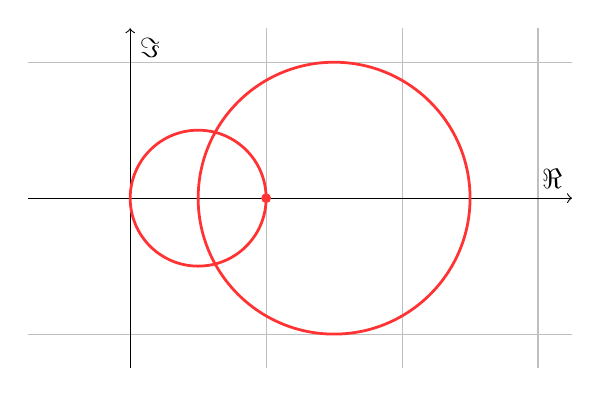
\begin{tikzpicture}
            \begin{axis}[
                    % xtick distance=2,
                    % ytick distance=2,
                    grid=major,
                    % grid style={line width=.1pt, draw=gray!10}%,major grid style={line width=.2pt,draw=gray!50}
                    ticks=none, % ticks aus?
                    axis lines = middle,
                    axis line style={->},
                    ymin=-2.5, ymax=2.5,
                    xmin=-1.5, xmax=6.5,
                    xlabel={$\Re$},
                    ylabel={$\Im$},
                    axis equal image,
                    width=0.7\textwidth
                ]
                \def\circlewidth{1pt}
                % A
                \draw[red!80, line width=\circlewidth] (axis cs:3,0) node[circle=2pt] {} circle (2);
                \draw[red!80, line width=\circlewidth, fill] (axis cs:2,0) circle (0.05);
                \draw[red!80, line width=\circlewidth] (axis cs:1,0) circle (1);

            \end{axis}
        \end{tikzpicture}
    \end{center}

    \[
        A^T =
        \left(
        \begin{array}{ccc}
                \cellcolor{red!20} 3 & \cellcolor{red!10} 0 & \cellcolor{red!10} 1 \\
                \cellcolor{red!10} 1 & \cellcolor{red!20} 2 & \cellcolor{red!10} 0 \\
                \cellcolor{red!10} 1 & \cellcolor{red!10} 0 & \cellcolor{red!20} 1
            \end{array}
        \right)
        \quad \implies \quad
        \begin{matrix}
            \cellcolor{red!20} m_1 = 3 &  & \cellcolor{red!10} r_1 = |0| + |1| = 1 \\
            \cellcolor{red!20} m_2 = 2 &  & \cellcolor{red!10} r_2 = |1| + |0| = 1 \\
            \cellcolor{red!20} m_2 = 1 &  & \cellcolor{red!10} r_3 = |1| + |0| = 1
        \end{matrix}
    \]

    \begin{center}
        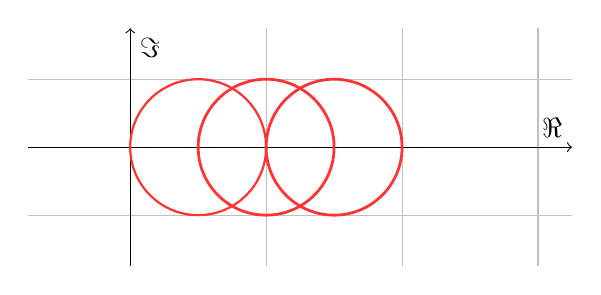
\begin{tikzpicture}
            \begin{axis}[
                    % xtick distance=2,
                    % ytick distance=2,
                    grid=major,
                    % grid style={line width=.1pt, draw=gray!10}%,major grid style={line width=.2pt,draw=gray!50}
                    ticks=none, % ticks aus?
                    axis lines = middle,
                    axis line style={->},
                    ymin=-1.75, ymax=1.75,
                    xmin=-1.5, xmax=6.5,
                    xlabel={$\Re$},
                    ylabel={$\Im$},
                    axis equal image,
                    width=0.7\textwidth
                ]
                \def\circlewidth{1pt}
                % A^T
                \draw[red!80, line width=\circlewidth] (axis cs:3,0) circle (1);
                \draw[red!80, line width=\circlewidth] (axis cs:2,0) circle (1);
                \draw[red!80, thick] (axis cs:1,0) circle (1);

            \end{axis}
        \end{tikzpicture}
    \end{center}
\end{example}

\begin{bonus}{Eigenwertproblem als Nullstellenproblem}
    Ist $A$ symmetrisch, so gelten zusätzlich folgende Aussagen:
    \begin{itemize}
        \item $\lambda_i \in \R, \forall i$
        \item es gibt $n$ Eigenvektoren $v_i$, die linear unabhängig sind, d.h. $A$ ist diagonalisierbar
        \item die $v_i$ können so gewählt werden, dass sie eine Orthonormalbasis bilden:
              \[
                  \langle v_i, v_j \rangle = \delta_{ij}, \quad i, j = 1, \ldots, n
              \]
        \item $Q = \begin{pmatrix}
                      v_1 & \ldots & v_n
                  \end{pmatrix}$ ist eine Orthonormalmatrix und es gilt:
              \[
                  A = Q \Lambda Q^{-1} = Q \Lambda Q^{T}, \quad \Lambda = \begin{pmatrix}
                      \lambda_1 &        &           \\
                                & \ddots &           \\
                                &        & \lambda_n
                  \end{pmatrix}
              \]
              bzw.
              \[
                  \Lambda = Q^T A Q
              \]
        \item da die $v_i$ eine Orthonormalbasis bilden, kann jeder Vektor $x \in \R^n$ geschrieben werden als
              \[
                  x = \sum_{i=1}^{n} x_i v_i, \quad x_i = \langle x, v_i \rangle
              \]
              und
              \[
                  Ax = \sum_{i=1}^{n} x_i A v_i = \sum_{i=1}^{n} \lambda_i x_i v_i
              \]
    \end{itemize}

    Das Eigenwertproblem ist also ein Nullstellenproblem für das Polynom $p_A$.

    Aus der Algebra wissen wir, dass es ab Polynomgrad 5 keinen endlichen Algorithmus zur Lösung dieses Problems gibt.
    Numerische Algorithmen können deswegen nur iterative Verfahren sein.
\end{bonus}

\subsection{Vektoriteration}

\begin{defi}{Vektoriteration}
    Die \emph{Vektoriteration} ist ein numerisches Verfahren zur Berechnung des betragsgrößten Eigenwertes und des dazugehörigen Eigenvektors einer Matrix.

    Wir wissen bereits, dass jedes $x \in \R^n$ als
    \[
        x = \sum_{i=1}^{n} x_i v_i, \quad x_i = \langle x, v_i \rangle
    \]
    geschrieben werden kann.
    Damit gilt:
    \[
        Ax = \sum_i \lambda_i x_i v_i \quad \implies \quad A^kx = \sum_i \lambda_i^k x_i v_i
    \]

    Gilt $|\lambda_1| > \dots > |\lambda_n|$, so dominiert der Anteil $\lambda_1 x_1 v_1$ (falls $x_1 \neq 0$) in $A^k x$.

    Wird $x$ oft genug mit $A$ multipliziert, so bleibt im wesentlichen ein Vielfaches von $v_1$ übrig.

    Ist $|\lambda_1| > 1$, so wird $\|A^kx\|_2$ immer größer.
    Um die damit verbundenen numerischen Probleme zu vermeiden normalisiert man nach jeder Multiplikation mit $A$ den neu berechneten Vektor und erhält somit die \emph{Vektoriteration}:
    \begin{enumerate}
        \item Wähle $x^{(0)}$ mit $\|x^{(0)}\|_2 = 1$ und $x_1^{(0)} = \langle x^{(0)}, v_1 \rangle \neq 0$
        \item Wiederhole:
              \[
                  y^{(k+1)} = A x^{(k)}
              \]
              \[
                  x^{(k+1)} = \frac{y^{(k+1)}}{ \| y^{(k+1)} \|_2 }
              \]
              \[
                  \mu^{(k+1)} = \langle x^{(k)}, y^{(k+1)} \rangle
              \]
    \end{enumerate}

    Ist $A$ symmetrisch mit $\lambda_1 > |\lambda_2| > \dots > |\lambda_n|$.
    Dann ist die Vektoriteration
    \[
        \mu^{(k)} \xrightarrow{k \to \infty} \lambda_1, \quad x^{(k)} \xrightarrow{k \to \infty} \sign(x_1^{(0)}) v_1
    \]
    falls $x_1^{(0)} = \langle x^{(0)}, v_1 \rangle \neq 0$ ist.
\end{defi}

\begin{example}{Vektoriteration}
    Gegeben seien eine Matrix $A$ und ein Startvektor $x^{(0)}$ mit:
    \[
        A =
        \begin{pmatrix}
            2 & 1 & 0 & 0 \\
            1 & 2 & 1 & 0 \\
            0 & 1 & 2 & 1 \\
            0 & 0 & 1 & 2
        \end{pmatrix}
        , \quad
        x^{(0)} =
        \begin{pmatrix}
            1 \\ 0 \\ 0 \\ 0
        \end{pmatrix}
    \]

    Wenden Sie die Vektoriteration an und berechnen Sie den betragsgrößten Eigenwert und den Eigenvektor.

    \exampleseparator

    $k = 1$:
    \[
        y^{(1)} = A x^{(0)} =
        \begin{pmatrix}
            2 & 1 & 0 & 0 \\
            1 & 2 & 1 & 0 \\
            0 & 1 & 2 & 1 \\
            0 & 0 & 1 & 2
        \end{pmatrix}
        \begin{pmatrix}
            1 \\ 0 \\ 0 \\ 0
        \end{pmatrix}
        =
        \begin{pmatrix}
            2 \\ 1 \\ 0 \\ 0
        \end{pmatrix}
    \]
    \[
        x^{(1)} = \frac{y^{(1)}}{ \| y^{(1)} \|_2 } = \frac{1}{\sqrt{5}}
        \begin{pmatrix}
            2 \\ 1 \\ 0 \\ 0
        \end{pmatrix}
        \approx
        \begin{pmatrix}
            0.89 \\ 0.45 \\ 0 \\ 0
        \end{pmatrix}
    \]
    \[
        \mu^{(1)} = \langle x^{(0)}, y^{(1)} \rangle = \langle
        \begin{pmatrix}
            1 \\ 0 \\ 0 \\ 0
        \end{pmatrix},
        \begin{pmatrix}
            2 \\ 1 \\ 0 \\ 0
        \end{pmatrix}
        \rangle
        = 2
    \]

    $k = 2$:
    \[
        y^{(2)} = A x^{(1)} = \frac{1}{\sqrt{5}}
        \begin{pmatrix}
            2 & 1 & 0 & 0 \\
            1 & 2 & 1 & 0 \\
            0 & 1 & 2 & 1 \\
            0 & 0 & 1 & 2
        \end{pmatrix}
        \begin{pmatrix}
            2 \\ 1 \\ 0 \\ 0
        \end{pmatrix}
        = \frac{1}{\sqrt{5}}
        \begin{pmatrix}
            5 \\ 4 \\ 1 \\ 0
        \end{pmatrix}
    \]
    \[
        x^{(2)} = \frac{y^{(2)}}{ \| y^{(2)} \|_2 } = \frac{1}{\sqrt{\frac{42}{5}}} \cdot \frac{1}{\sqrt{5}}
        \begin{pmatrix}
            5 \\ 4 \\ 1 \\ 0
        \end{pmatrix}
        = \frac{1}{\sqrt{42}}
        \begin{pmatrix}
            5 \\ 4 \\ 1 \\ 0
        \end{pmatrix}
        \approx
        \begin{pmatrix}
            0.77 \\ 0.62 \\ 0.15 \\ 0
        \end{pmatrix}
    \]
    \[
        \mu^{(2)} = \langle x^{(1)}, y^{(2)} \rangle = \frac{1}{5} \langle
        \begin{pmatrix}
            2 \\ 1 \\ 0 \\ 0
        \end{pmatrix},
        \begin{pmatrix}
            5 \\ 4 \\ 1 \\ 0
        \end{pmatrix}
        \rangle
        = 2.8
    \]

    $\ldots$

    $k = 15$:
    \[
        x^{(15)} \approx
        \begin{pmatrix}
            0.3793 \\ 0.6061 \\ 0.5968 \\ 0.3641
        \end{pmatrix}
        , \quad
        \mu^{(15)} \approx 3.6177
    \]
\end{example}

\subsection{Jacobi-Verfahren}

\begin{defi}{Jacobi-Verfahren (Eigenwerte)}
    Die Idee des \emph{Jacobi-Verfahrens} besteht darin, das jeweils betragsgrößte Außerdiagonalelement mit Hilfe einer Givens-Rotation auf $0$ zu bringen, und sich auf diese Art mehr und mehr einer Diagonalmatrix anzunähern.

    Es ergibt sich die Iterationsvorschrift:
    \begin{enumerate}
        \item $A^{0} = A$
        \item Wiederhole:
              \[
                  A^{(k+1)} = {Q^{(k)}}^T A^{(k)} Q^{(k)} = \underbrace{Q_k^T \cdot \ldots \cdot Q_1^T}_{{Q^{(k)}}^T} A^{(0)} \underbrace{Q_1 \cdot \ldots \cdot Q_k}_{Q^{(k)}}
              \]
              $Q_k$ wird wie folgt bestimmt:
              \begin{itemize}
                  \item suche das betragsgrößte Nebendiagonalelement $a_{i_0 j_0}^{(k-1)}$ von $A^{k-1}$
                  \item dabei kann $j_0 > i_0$ angenommen werden, da alle Matrizen $A^{k-1}$ symmetrisch sind
                  \item bestimme $Q_k$ so, dass $a_{i_0 j_0}^{(k)} = 0$, also
                        \[
                            Q_k =
                            \begin{pmatrix}
                                1 &        &   &    &   &        &   &   &   &        &   \\
                                  & \ddots &   &    &   &        &   &   &   &        &   \\
                                  &        & 1 &    &   &        &   &   &   &        &   \\
                                  &        &   & c  &   &        &   & s &   &        &   \\
                                  &        &   &    & 1 &        &   &   &   &        &   \\
                                  &        &   &    &   & \ddots &   &   &   &        &   \\
                                  &        &   &    &   &        & 1 &   &   &        &   \\
                                  &        &   & -s &   &        &   & c &   &        &   \\
                                  &        &   &    &   &        &   &   & 1 &        &   \\
                                  &        &   &    &   &        &   &   &   & \ddots &   \\
                                  &        &   &    &   &        &   &   &   &        & 1
                            \end{pmatrix}
                        \]
                        mit
                        \[
                            \alpha = \frac{a_{j_0 j_0} - a_{i_0 i_0}}{2 a_{i_0 j_0}} \quad \implies \quad c = \sqrt{\frac{1}{2} + \frac{1}{2} \sqrt{\frac{\alpha^2}{1 + \alpha^2}}}, \quad s = \frac{\sign(\alpha)}{2c \sqrt{1 + \alpha^2}}
                        \]
              \end{itemize}
    \end{enumerate}

    Dann ist ($\lambda_i$ Eigenwerte, $v_i$ Eigenvektoren)
    \[
        \diagonal(A^{(k)}) =
        \begin{pmatrix}
            a_{11}^{(k)} &        &              \\
                         & \ddots &              \\
                         &        & a_{nn}^{(k)}
        \end{pmatrix}
        \approx
        \begin{pmatrix}
            \lambda_1 &        &           \\
                      & \ddots &           \\
                      &        & \lambda_n
        \end{pmatrix}
        = \Lambda
    \]
    \[
        Q^{(k)} \approx
        \begin{pmatrix}
            v_1 & \ldots & v_n
        \end{pmatrix}
    \]
\end{defi}

\begin{example}{Jacobi-Verfahren}
    Gegeben sei die Matrix $A$ mit:
    \[
        A =
        \begin{pmatrix}
            3 & 4 \\
            4 & 3
        \end{pmatrix}
    \]

    Führen Sie das Jacobi-Verfahren für eine Iteration aus und berechnen Sie die Eigenwerte (näherungsweise).

    \exampleseparator

    \[
        A = A^{(0)} =
        \left(
        \begin{array}{cc}
                3 & \cellcolor{red!20} 4 \\
                4 & 3
            \end{array}
        \right)
        \quad \implies \quad
        i_0 = 1, \quad j_0 = 2
    \]

    Damit gilt:
    \[
        Q_1 =
        \begin{pmatrix}
            c  & s \\
            -s & c
        \end{pmatrix}
    \]
    mit
    \[
        \alpha = \frac{a_{j_0 j_0} - a_{i_0 i_0}}{2 a_{i_0 j_0}} = \frac{a_{22} - a_{11}}{2 a_{1 2}} = \frac{3 - 3}{2 \cdot 4} = 0
    \]
    \[
        \implies \quad c = \sqrt{\frac{1}{2} + \frac{1}{2} \sqrt{\frac{\alpha^2}{1 + \alpha^2}}} = \sqrt{\frac{1}{2}} = \frac{1}{\sqrt{2}}, \quad s = \frac{\sign(\alpha)}{2c \sqrt{1 + \alpha^2}} = \frac{1}{2 \cdot \frac{1}{\sqrt{2}} \cdot \sqrt{1}} = \frac{1}{\sqrt{2}}
    \]
    \[
        \implies \quad Q_1 =
        \left(
        \begin{array}{cc}
                \cellcolor{red!10} \nicefrac{1}{\sqrt{2}}  & \cellcolor{blue!10} \nicefrac{1}{\sqrt{2}} \\
                \cellcolor{red!10} -\nicefrac{1}{\sqrt{2}} & \cellcolor{blue!10} \nicefrac{1}{\sqrt{2}}
            \end{array}
        \right)
    \]
    \[
        \implies \quad A^{(1)} = Q_1^T A^{(0)} Q_1 =
        \begin{pmatrix}
            \nicefrac{1}{\sqrt{2}} & -\nicefrac{1}{\sqrt{2}} \\
            \nicefrac{1}{\sqrt{2}} & \nicefrac{1}{\sqrt{2}}
        \end{pmatrix}
        \begin{pmatrix}
            3 & 4 \\
            4 & 3
        \end{pmatrix}
        \begin{pmatrix}
            \nicefrac{1}{\sqrt{2}}  & \nicefrac{1}{\sqrt{2}} \\
            -\nicefrac{1}{\sqrt{2}} & \nicefrac{1}{\sqrt{2}}
        \end{pmatrix}
        = \ldots =
        \left(
        \begin{array}{cc}
                \cellcolor{red!20} -1 & 0                     \\
                0                     & \cellcolor{blue!20} 7
            \end{array}
        \right)
    \]

    Damit erhalten wir die Eigenwerte und dazugehörigen Eigenvektoren:
    \[
        \lambda_1 = -1, \quad v_1 =
        \begin{pmatrix}
            \nicefrac{1}{\sqrt{2}} \\ -\nicefrac{1}{\sqrt{2}}
        \end{pmatrix}
    \]
    \[
        \lambda_2 = 7, \quad v_2 =
        \begin{pmatrix}
            \nicefrac{1}{\sqrt{2}} \\ \nicefrac{1}{\sqrt{2}}
        \end{pmatrix}
    \]
\end{example}

\subsection{QR-Verfahren, Hessenberg-Transformation, Shift-Technik}

\begin{defi}{QR-Verfahren (singuläre Matrizen)}
    Mit Givens- bzw. Householder-Transformationen können wir eine \emph{reguläre Matrix} $A$ in $A = QR$ zerlegen, wobei $Q$ orthonormal und $R$ eine obere Dreiecksmatrix ist.

    Eine analoge Zerlegung ist auch für \emph{singuläres} $A$ möglich:
    \begin{itemize}
        \item Falls eine Spalte inklusive des Diagonalelements gleich $0$ ist, benutzt man als Dreh- bzw. Spiegelmatrix $Q_k = I$.
        \item Auf der Diagonalen der oberen Dreiecksmatrix $R$ trägt man entsprechend eine $0$ ein.
        \item Wir zerlegen eine beliebige quadratische Matrix $A$ in $A = QR$ und betrachten
              \[
                  RQ = Q^T Q R Q = Q^T A Q
              \]
        \item Da $Q^T = Q^{-1}$ ist, gilt
              \[
                  RQ = Q^{-1} A Q
              \]
              d. h. $RQ$ und $A = QR$ haben die selben Eigenwerte.
        \item Wir bauen daraus wie üblich eine Iteration auf und erhalten das \emph{QR-Verfahren}:
              \begin{enumerate}
                  \item Starte mit $A^{(0)} = A$
                  \item Wiederhole:
                        \begin{enumerate}
                            \item Zerlege
                                  \[
                                      A^{(k)} = Q_k R_k
                                  \]
                            \item Berechne
                                  \[
                                      A^{(k+1)} = R_k Q_k
                                  \]
                        \end{enumerate}
              \end{enumerate}
    \end{itemize}

    Bei symmetrischem $A$ konvergieren die $A^{(k)}$ wie bei Jacobi gegen die Diagonalmatrix $\Lambda$ und die Spalten von $Q^{(k)}$ können wieder als Approximationen der Eigenvektoren benutzt werden.
\end{defi}

\begin{defi}{Hessenberg-Form}
    Eine (obere) \emph{Hessenbergmatrix} ist eine quadratische Matrix $H \in \R^{n \times n}$, deren Einträge unterhalb der ersten Nebendiagonalen gleich Null sind, also $h_{ij} = 0$ für alle $i > j + 1$:
    \[
        H =
        \begin{pmatrix}
            h_{11} & h_{12} & h_{13} & \cdots   & h_{1n} \\
            h_{21} & h_{22} & h_{23} & \cdots   & h_{2n} \\
            0      & h_{32} & h_{33} & \cdots   & h_{3n} \\
            \vdots & \ddots & \ddots & \ddots   & \vdots \\
            0      & \cdots & 0      & h_{nn-1} & h_{nn}
        \end{pmatrix}
    \]

    Analog definiert man die untere Hessenbergmatrix als eine quadratische Matrix, deren Transponierte eine obere Hessenbergmatrix ist.

    Ist nur von einer Hessenbergmatrix die Rede, ist meist eine obere Hessenbergmatrix gemeint.

    Eine Matrix, die sowohl eine untere als auch eine obere Hessenbergmatrix ist, ist eine Tridiagonalmatrix.
\end{defi}

\begin{bonus}{Hessenberg-Form und QR-Verfahren}
    Der Aufwand beim QR-Verfahren entspricht pro Schritt im wesentlichen einer Householder-Zerlegung $(\approx \frac{4}{3} n^3)$ und ist damit extrem hoch.

    Für das QR-Verfahren bringt die Hessenberg-Form folgenden Vorteil:

    Bei der QR-Zerlegung einer Hessenberg-Matrix muss pro Spalte nur das Subdiagonalelement eliminiert werden, was jeweils mit einer einzigen Givens-Rotation erledigt werden kann, so dass der Gesamtaufwand nur noch $\approx n^2$ statt $\approx \frac{4}{3} n^3$ ist.

    Hat $A^{(k)}$ Hessenberg-Form und wurde mit Givens-Matrizen in $A^{(k)} = Q_k R_k$ zerlegt, so hat sowohl $Q_k$ als auch $A^{(k+1)} = R_k Q_k$ wieder Hessenberg-Form.

    Ist $A$ symmetrisch, so vereinfacht sich das ganze nochmals:
    \begin{itemize}
        \item Die Hessenberg-Transformierte $H$ ist wegen $H = QAQ^{-1} = QAQ^T$ ebenfalls symmetrisch und muss deshalb tridiagonal sein.
        \item Wird das QR-Verfahren mit tridiagonalem $A^{(0)}$ gestartet, so sind alle $A^{(k)}$ tridiagonal und der Aufwand für die Zerlegung $A^{(k)} = Q_k R_k$ und die Matrixmultiplikation $Q_k R_k$ ist $\approx n$.
    \end{itemize}
\end{bonus}

\begin{defi}{Hessenberg-Transformation}
    Gegeben sei eine Matrix $A \in \R^{n \times n}$ und $\tilde{A} \in \R^{n-1 \times n}$ eine Untermatrix von $A$, konstruiert durch Entfernen der ersten Zeile von $A$, und $\tilde{a}_1$ die erste Spalte von $\tilde{A}$.

    Wir konstruieren dann die Householder-Matrix $\tilde{Q}_1$, die $\tilde{a}_1$ eliminiert, d.h.
    \[
        \tilde{Q}_1 \tilde{a}_1 = \alpha_1 \begin{pmatrix}
            1 \\ 0 \\ \vdots \\ 0
        \end{pmatrix}
    \]

    Wir erweitern $\tilde{Q}_1$ auf die gesamte orthonormale Matrix $Q_1 \in \R^{n \times b}$, d.h.
    \[
        Q_1 = \begin{bmatrix}
            1 & 0           \\
            0 & \tilde{Q}_1 \\
        \end{bmatrix}
    \]

    Dann gilt
    \[
        Q_1 A = \begin{pmatrix}
            a_{11}   & *      & \cdots & \cdots & *      \\
            \alpha_1 & *      & \cdots & \cdots & *      \\
            0        & \vdots &        &        & \vdots \\
            \vdots   & \vdots &        &        & \vdots \\
            0        & *      & \cdots & \cdots & *
        \end{pmatrix}
        , \quad
        Q_1 A Q_1^T = Q_1 A Q_1^{-1} = \begin{pmatrix}
            a_{11}   & *      & \cdots & \cdots & *      \\
            \alpha_1 & *      & \cdots & \cdots & *      \\
            0        & \vdots &        &        & \vdots \\
            \vdots   & \vdots &        &        & \vdots \\
            0        & *      & \cdots & \cdots & *
        \end{pmatrix}
    \]

    Analoges Vorgehen für Spalte $2$ bis $n-2$ liefert
    \[
        H = \underbrace{Q_{n-2} \cdot \ldots \cdot Q_1}_{Q} A \underbrace{Q_1^T \cdot \ldots \cdot Q_{n-2}^T}_{Q^T = Q^{-1}} = \begin{pmatrix}
            *      & \cdots & \cdots & \cdots & *      \\
            *      & \ddots &        &        & \vdots \\
            0      & \ddots & \ddots &        & \vdots \\
            \vdots & \ddots & \ddots & \ddots & \vdots \\
            0      & \cdots & 0      & *      & *
        \end{pmatrix}
    \]

    $H = Q A Q^{-1}$ hat dieselben Eigenwerte wie $A$ und besitzt Hessenberg-Form, d.h. das um die erste Nebendiagonale reduzierte untere Dreieck ist identisch $0$.
\end{defi}

\begin{example}{Hessenberg-Transformation}
    TODO
\end{example}

\begin{bonus}{QR-Verfahren mit einfachen Shifts}
    Mit der Hessenberg-Transformation haben wir den Aufwand reduziert, aber die Konvergenzgeschwindigkeit kann noch verbessert werden.
    Dazu benutzen wir den folgenden Zusammenhang:

    Zerlege statt $A$ die Matrix
    \[
        A - \mu I = QR
    \]
    Dann hat
    \[
        \tilde{A} = RQ + \mu I
    \]
    wegen $Q^T = Q^{-1}$ dieselben Eigenwerte wie $A$, denn
    % \begin{alignat*}{1}
    %     \tilde{A} & = RQ + \mu I                    \\
    %               & = Q^T Q R Q + \mu I             \\
    %               & = Q^T (A - \mu I) Q + \mu I     \\
    %               & = Q^T A Q - \mu Q^T I Q + \mu I \\
    %               & = Q^T A Q - \mu I + \mu I       \\
    %               & = Q^T A Q
    % \end{alignat*}
    \[
        \tilde{A} = RQ + \mu I = Q^T Q R Q + \mu I = Q^T (A - \mu I) Q + \mu I = Q^T A Q - \mu Q^T I Q + \mu I =  Q^T A Q
    \]

    Damit bauen wir in das QR-Verfahren einen \emph{Shift} ein, d.h. wir ändern die Iteration wie folgt:
    \begin{enumerate}
        \item Starte mit $A^{(0)} = A$ in Hessenberg-Form
        \item Wiederhole:
              \begin{enumerate}
                  \item Zerlege
                        \[
                            A^{(k)} - \mu^{(k)} I = Q_k R_k
                        \]
                  \item Berechne
                        \[
                            A^{(k+1)} = R_k Q_k + \mu^{(k)} I
                        \]
              \end{enumerate}
    \end{enumerate}
    wobei $\mu^{(k)}$ geeignet zu bestimmen ist.

    Üblicherweise wird versucht, mit dem Shift $\mu^{(k)}$ den betragskleinsten Eigenwert $\lambda_n$ zu approximieren.
    Dazu kann das letzte Diagonalelement $\mu^{(k)} = (A^{(k)})_{nn}$ gewählt werden.

    Mit dieser Wahl konvergiert $a^{(k)}_{nn-1}$ schnell gegen $0$ und $a^{(k)}_{nn}$ gegen $\lambda_n$ von $A$, d.h. ist $l > k$ groß genug, dann ist
    \[
        A^{(l)} = \begin{pmatrix}
            *      & \cdots & \cdots & \cdots   & *                 \\
            *      & \ddots &        &          & \vdots            \\
            0      & \ddots & \ddots &          & \vdots            \\
            \vdots & \ddots & *      & *        & *                 \\
            0      & \cdots & 0      & \epsilon & \tilde{\lambda}_n
        \end{pmatrix}
    \]
    wobei $\epsilon \approx 0$ nd $\tilde{\lambda}_n \approx \lambda_n$ ist.

    Damit haben wir einen Eigenwert approximiert und die restlichen Eigenwerte sind ausschließlich durch die ersten $n-1$ Spalten und Zeilen der Matrix bestimmt.
    Deshalb streichen wir die letzte Zeile und Spalte und wiederholen das Verfahren auf der verbliebenen Restmatrix.

    Diese Reduktionstechnik nennt sich \emph{Deflation}.

    Die Implementierung in dieser Form zählt zu den Standardverfahren und findet sich so auch in den einschlägigen Bibliotheken (z.B. \texttt{LAPACK}).

    Die einfache QR-Iteration ergibt sich, indem alle Shifts zu Null gesetzt werden.
\end{bonus}
\section{Nichtlineare Gleichungen}

%\subsection{Einleitung}

\subsection{Einfache Verfahren und ihre geometrische Interpretation}
\subsubsection{Bisektions-Verfahren}

% \begin{defi}{Einschließungsverfahren}
%     Verfahren, die untere und obere Schranken $a_k$ und $b_k$ für eine gesuchte Nullstelle erzeugen, nennt man \emph{Einschließungsverfahren}.
% \end{defi}

\begin{defi}{Bisektions-Verfahren}
    Wir setzen $f: \R \to \R$ stetig voraus.
    
    Ist $f(a_0) \cdot f(b_0) < 0$, dann muss in $[a_0, b_0]$ \emph{mindestens} eine Nullstelle von $f$ liegen.
    
    Betrachte $x_0 = \frac{a_0 + b_0}{2}$, also die Intervallmitte.
    
    Wiederhole solange, bis die Intervalllänge $|b_i - a_i|$ oder $|f(x_i)|$ hinreichend klein ist:
    \begin{itemize}
        \item Berechne
              \[
                  x_{i} = \frac{a_i + b_i}{2}
              \]
        \item Setze
              \[
                  \begin{cases}
                      a_{i+1} = a_{i}, \quad b_{i+1} = x_{i} & \text{falls } f(a_{i}) \cdot f(x_{i}) < 0 \\
                      a_{i+1} = x_{i}, \quad b_{i+1} = b_{i} & \text{sonst}
                  \end{cases}
              \]
        \item Betrachte nun $[a_{i+1}, b_{i+1}]$
    \end{itemize}
    
    Das Bisektions-Verfahren ist ein Einschließungsverfahren.
\end{defi}

\begin{example}{Bisektions-Verfahren}
    Gegeben sei die Funktion $f(x)$ und das Intervall $[a_0, b_0]$ mit: 
    \[ 
        f(x) = x^2 - 3, \quad a_0 = 0, \quad b_0 = 2
    \]
    
    Führen Sie das Bisektions-Verfahren durch.
    
    \exampleseparator
    
    $k = 0$:
    \[ 
        x_0 = \frac{a_0 + b_0}{2} = \frac{0 + 2}{2} = 1
    \]
    \[ 
        f(a_0) \cdot f(x_0) = -3 \cdot (-2) = 6 \geq 0 \quad \implies \quad a_1 = x_0 = 1, \quad b_1 = b_0 = 2
    \]
    
    $k = 1$:
    \[ 
        x_1 = \frac{a_1 + b_1}{2} = \frac{1 + 2}{2} = \frac{3}{2}
    \]
    \[ 
        f(a_1) \cdot f(x_1) = -2 \cdot \left(-\frac{3}{4}\right) = \frac{3}{2} \geq 0 \quad \implies \quad a_2 = x_1 = \frac{3}{2}, \quad b_2 = b_1 = 2
    \]
    
    $k = 2$:
    \[ 
        x_2 = \frac{a_2 + b_2}{2} = \frac{\frac{3}{2} + 2}{2} = \frac{7}{4}
    \]
    \[ 
        f(a_2) \cdot f(x_2) = \frac{1}{16} \cdot 1 = -\frac{1}{16} < 0 \quad \implies \quad a_3 = a_2 = \frac{3}{2}, \quad b_3 = x_2 = \frac{7}{4}
    \]
    
    usw.
    
    \begin{center}
        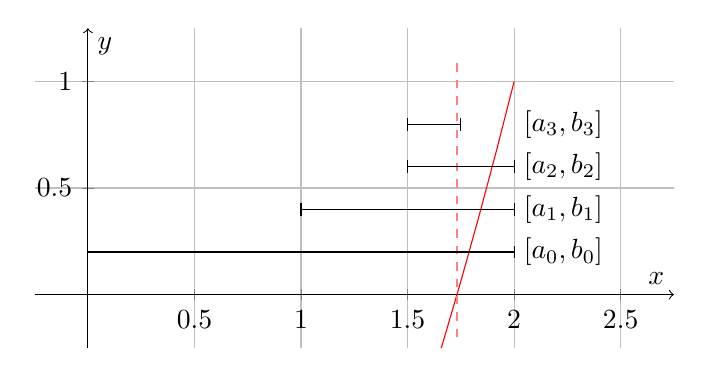
\begin{tikzpicture}
            \begin{axis}[
                    % xtick distance=2,
                    % ytick distance=2,
                    grid=major,
                    % grid style={line width=.1pt, draw=gray!10}%,major grid style={line width=.2pt,draw=gray!50}
                    % ticks=none, % ticks aus?
                    axis lines = middle,
                    axis line style={->},
                    ymin=-0.25, ymax=1.25,
                    xmin=-0.25, xmax=2.75,
                    xlabel={$x$},
                    ylabel={$y$},
                    axis equal image,
                    width=0.8\textwidth,
                    domain=0:2,
                ]
                % f = x^2-3
                \addplot[no marks, red]{x^2-3};
                \draw[red!50, dashed] (axis cs:1.73205,-0.2) -- (axis cs:1.73205,1.1);
                
                
                \draw (axis cs:0,0.2) -- (axis cs:2,0.2);
                \draw (axis cs:0,0.17) -- (axis cs:0,0.23);
                \draw (axis cs:2,0.17) -- (axis cs:2,0.23);
                
                \draw (axis cs:1,0.4) -- (axis cs:2,0.4);
                \draw (axis cs:1,0.37) -- (axis cs:1,0.43);
                \draw (axis cs:2,0.37) -- (axis cs:2,0.43);
                
                \draw (axis cs:1.5,0.6) -- (axis cs:2,0.6);
                \draw (axis cs:1.5,0.57) -- (axis cs:1.5,0.63);
                \draw (axis cs:2,0.57) -- (axis cs:2,0.63);
                
                \draw (axis cs:1.5,0.8) -- (axis cs:7/4,0.8);
                \draw (axis cs:1.5,0.77) -- (axis cs:1.5,0.83);
                \draw (axis cs:7/4,0.77) -- (axis cs:7/4,0.83);
                
                
                % labels
                \node[right] at (axis cs:2,0.2) {$[a_0, b_0]$};
                \node[right] at (axis cs:2,0.4) {$[a_1, b_1]$};
                \node[right] at (axis cs:2,0.6) {$[a_2, b_2]$};
                \node[right] at (axis cs:2,0.8) {$[a_3, b_3]$};
            \end{axis}
        \end{tikzpicture}
    \end{center}
\end{example}

\subsubsection{Regula-Falsi-Verfahren}

\begin{bonus}{Regula-Falsi-Verfahren (Idee)}
    Wir modifizieren das Bisektions-Verfahren, um die Konvergenzgeschwindigkeit zu erhöhen.
    
    Benutze für $x_k$ nicht die Intervallmitte, sondern zusätzliche Information:
    \begin{itemize}
        \item verbinde $(a_k, f(a_k))$ und $(b_k, f(b_k))$ durch eine Gerade $s$
        \item $x_k$ sei jetzt die Nullstelle der Geraden $s$ mit
              \[
                  s(x) = f(a_k) + \frac{f(b_k) - f(a_k)}{b_k - a_k} \cdot (x - a_k)
              \]
              \[
                  s(x_k) = 0 \quad \iff \quad x_k = a_k - \frac{b_k - a_k}{f(b_k) - f(a_k)} = \frac{a_k f(b_k) - b_k f(a_k)}{f(b_k) - f(a_k)}
              \]
    \end{itemize}
\end{bonus}

\begin{defi}{Regula-Falsi-Verfahren}
    Das \emph{Regula-Falsi-Verfahren} funktioniert analog zum Bisektions-Verfahren, nur dass $x_k$ wie folgt berechnet wird:
    \[
        x_k = \frac{a_k f(b_k) - b_k f(a_k)}{f(b_k) - f(a_k)}
    \]
    
    Wiederhole solange, bis die Intervalllänge $|x_{i+1} - x_i|$ oder $|f(x_i)|$ hinreichend klein ist:\footnote{Anderes Abbruchkriterium als beim Bisektions-Verfahren!}
    \begin{itemize}
        \item Berechne
              \[
                  x_{i} = \frac{a_k f(b_k) - b_k f(a_k)}{f(b_k) - f(a_k)}
              \]
        \item Setze
              \[
                  \begin{cases}
                      a_{i+1} = a_{i}, \quad b_{i+1} = x_{i} & \text{falls } f(a_{i}) \cdot f(x_{i}) < 0 \\
                      a_{i+1} = x_{i}, \quad b_{i+1} = b_{i} & \text{sonst}
                  \end{cases}
              \]
        \item Betrachte nun $[a_{i+1}, b_{i+1}]$
    \end{itemize}
    
    Das Regula-Falsi-Verfahren ist ein Einschließungsverfahren.
\end{defi}

\begin{example}{Regula-Falsi-Verfahren}
    Gegeben sei die Funktion $f(x)$ und das Intervall $[a_0, b_0]$ mit: 
    \[ 
        f(x) = x^2 - 3, \quad a_0 = 0, \quad b_0 = 2
    \]
    
    Führen Sie das Regula-Falsi-Verfahren durch.
    
    \exampleseparator
    
    $k = 0$:
    \[ 
        x_{0} = \frac{a_0 f(b_0) - b_0 f(a_0)}{f(b_0) - f(a_0)} = \frac{0 - 2 \cdot (-3)}{1 - (-3)} = \frac{3}{2}
    \]
    \[ 
        f(a_0) \cdot f(x_0) = -3 \cdot \left(-\frac{3}{4}\right) = \frac{9}{4} \geq 0 \quad \implies \quad a_1 = x_0 = \frac{3}{2}, \quad b_1 = b_0 = 2
    \]
    
    $k = 1$:
    \[ 
        x_{1} = \frac{a_1 f(b_1) - b_1 f(a_1)}{f(b_1) - f(a_1)} = \frac{\frac{3}{2} \cdot 1 - 2 \cdot \left(-\frac{3}{4}\right)}{1 - \left(-\frac{3}{4}\right)} = \frac{12}{7}
    \]
    \[ 
        f(a_1) \cdot f(x_1) = -\frac{3}{4} \cdot \left(-\frac{3}{49}\right) = \ldots \geq 0 \quad \implies \quad a_2 = x_1 = \frac{12}{7}, \quad b_2 = b_1 = 2
    \]
    
    $k = 2$:
    \[ 
        x_{2} = \frac{a_2 f(b_2) - b_2 f(a_2)}{f(b_2) - f(a_2)} = \frac{\frac{12}{7} \cdot 1 - 2 \cdot \left(-\frac{3}{49}\right)}{1 - \left(-\frac{3}{49}\right)} = \frac{45}{26}
    \]
    \[ 
        f(a_2) \cdot f(x_2) = -\frac{3}{49} \cdot \left(-\frac{3}{676}\right) = \ldots \geq 0 \quad \implies \quad a_3 = x_2 = \frac{45}{26}, \quad b_2 = b_1 = 2
    \]
    
    usw.
    
    \begin{center}
        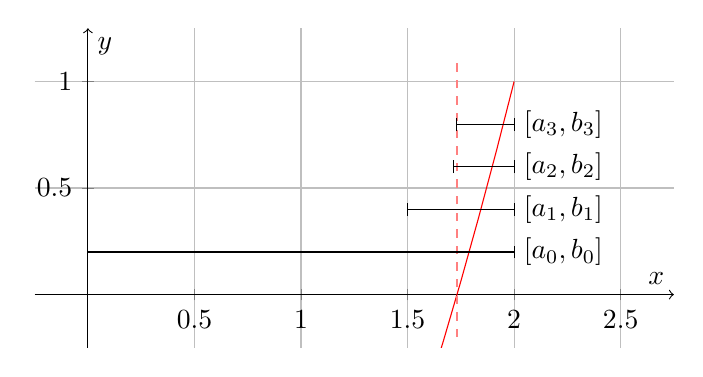
\begin{tikzpicture}
            \begin{axis}[
                    % xtick distance=2,
                    % ytick distance=2,
                    grid=major,
                    % grid style={line width=.1pt, draw=gray!10}%,major grid style={line width=.2pt,draw=gray!50}
                    % ticks=none, % ticks aus?
                    axis lines = middle,
                    axis line style={->},
                    ymin=-0.25, ymax=1.25,
                    xmin=-0.25, xmax=2.75,
                    xlabel={$x$},
                    ylabel={$y$},
                    axis equal image,
                    width=0.8\textwidth,
                    domain=0:2,
                ]
                % f = x^2-3
                \addplot[no marks, red]{x^2-3};
                \draw[red!50, dashed] (axis cs:1.73205,-0.2) -- (axis cs:1.73205,1.1);
                
                \draw (axis cs:0,0.2) -- (axis cs:2,0.2);
                \draw (axis cs:0,0.17) -- (axis cs:0,0.23);
                \draw (axis cs:2,0.17) -- (axis cs:2,0.23);
                
                \draw (axis cs:3/2,0.4) -- (axis cs:2,0.4);
                \draw (axis cs:3/2,0.37) -- (axis cs:3/2,0.43);
                \draw (axis cs:2,0.37) -- (axis cs:2,0.43);
                
                \draw (axis cs:12/7,0.6) -- (axis cs:2,0.6);
                \draw (axis cs:12/7,0.57) -- (axis cs:12/7,0.63);
                \draw (axis cs:2,0.57) -- (axis cs:2,0.63);
                
                \draw (axis cs:45/26,0.8) -- (axis cs:2,0.8);
                \draw (axis cs:45/26,0.77) -- (axis cs:45/26,0.83);
                \draw (axis cs:2,0.77) -- (axis cs:2,0.83);
                
                % labels
                \node[right] at (axis cs:2,0.2) {$[a_0, b_0]$};
                \node[right] at (axis cs:2,0.4) {$[a_1, b_1]$};
                \node[right] at (axis cs:2,0.6) {$[a_2, b_2]$};
                \node[right] at (axis cs:2,0.8) {$[a_3, b_3]$};
            \end{axis}
        \end{tikzpicture}
    \end{center}
\end{example}

\subsubsection{Sekanten-Verfahren}

\begin{defi}{Sekanten-Verfahren}
    Wir erhalten das \emph{Sekanten-Verfahren}, indem wir das Regula-Falsi-Verfahren leicht abändern.
    
    Seien $x_{-2}, x_{-1}$ gegeben.
    Bestimme für $k = 0, 1, \ldots$ die neue Näherung $x_k$ als Nullstelle der Geraden durch die Punkte
    \[
        x_k = x_{k-2} - \frac{x_{k-1} - x_{k-2}}{f(x_{k-1}) - f(x_{k-2})} \cdot f(x_{k-2}) = x_{k-1} - \frac{x_{k-1} - x_{k-2}}{f(x_{k-1}) - f(x_{k-2})} \cdot f(x_{k-1})
    \]
    
    Das Sekanten-Verfahren ist \emph{kein} Einschließungsverfahren.
\end{defi}

\begin{bonus}{Konvergenz des Sekanten-Verfahrens}
    Ist $f$ zweimal stetig differenzierbar in einer hinreichend kleinen Umgebung $X$ der gesuchten Nullstelle $x$.
    
    Dann konvergiert das Sekanten-Verfahren für alle $x_{-2}, x_{-1} \in X$ und es gibt eine Konstante $c > 0$ so dass
    \[
        |e_k| \leq c |e_{k-1}|^{\frac{1+\sqrt{2}}{2}}, \quad k \to \infty
    \]
\end{bonus}

\begin{example}{Sekanten-Verfahren}
    Gegeben sei die Funktion $f(x)$ und die Punkte $x_{-2}, x_{-1}$ mit: 
    \[ 
        f(x) = x^2 - 3, \quad x_{-2} = 0, \quad x_{-1} = 2
    \]
    
    Führen Sie das Sekanten-Verfahren durch.
    
    \exampleseparator
    
    $k = 0$:
    \[
        x_0 = x_{-1} - \frac{x_{-1} - x_{-2}}{f(x_{-1}) - f(x_{-2})} \cdot f(x_{-1}) = 2 - \frac{2 - 0}{1 - (-3)} \cdot 1 = \frac{3}{2}
    \]
    
    $k = 1$:
    \[
        x_1 = x_{0} - \frac{x_{0} - x_{-1}}{f(x_{0}) - f(x_{-1})} \cdot f(x_{0}) = \frac{3}{2} - \frac{\frac{3}{2} - 2}{-\frac{3}{4} - 1} \cdot \left(-\frac{3}{4}\right) = \frac{12}{7}
    \]
    
    $k = 2$:
    \[
        x_2 = x_{1} - \frac{x_{1} - x_{0}}{f(x_{1}) - f(x_{0})} \cdot f(x_{1}) = \frac{12}{7} - \frac{\frac{12}{7} - \frac{3}{2}}{-\frac{3}{49} - \left(-\frac{3}{4}\right)} \cdot \left(-\frac{3}{49}\right) = \frac{26}{15}
    \]
    
    usw.
    
    \begin{center}
        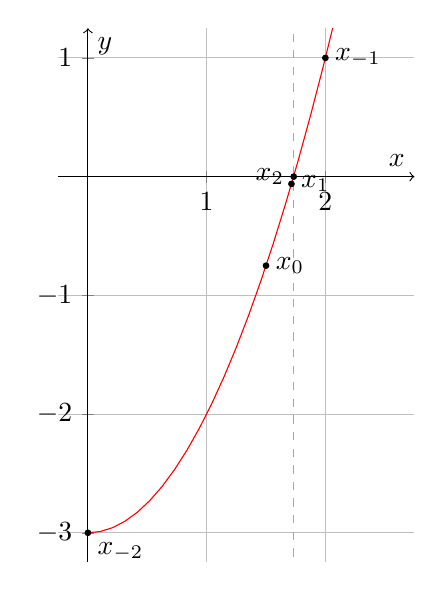
\begin{tikzpicture}
            \begin{axis}[
                    % xtick distance=2,
                    % ytick distance=2,
                    grid=major,
                    % grid style={line width=.1pt, draw=gray!10}%,major grid style={line width=.2pt,draw=gray!50}
                    % ticks=none, % ticks aus?
                    axis lines = middle,
                    axis line style={->},
                    ymin=-3.25, ymax=1.25,
                    xmin=-0.25, xmax=2.75,
                    xlabel={$x$},
                    ylabel={$y$},
                    axis equal image,
                    width=0.8\textwidth,
                    domain=0:2.5,
                ]
                % f = x^2-3
                \addplot[no marks, red]{x^2-3};
                \draw[red!50, dashed] (axis cs:1.73205,-3.2) -- (axis cs:1.73205,1.2);
                
                \draw[fill, black] (axis cs: 0, -3) circle (1pt) node[below right] {$x_{-2}$};
                \draw[fill, black] (axis cs: 2, 2^2-3) circle (1pt) node[right] {$x_{-1}$};
                \draw[fill, black] (axis cs: 3/2, 1.5^2-3) circle (1pt) node[right] {$x_{0}$};
                \draw[fill, black] (axis cs: 12/7, 1.7143^2-3) circle (1pt) node[right] {$x_{1}$};
                \draw[fill, black] (axis cs: 26/15, 0) circle (1pt) node[left] {$x_{2}$};
            \end{axis}
        \end{tikzpicture}
    \end{center}
\end{example}

\subsubsection{Taylor-Reihen-basierte Verfahren, Newton-Verfahren}

\begin{bonus}{Wiederholung Taylor-Entwicklung}
    Ist $f(x) = 0$ und $f$ hinreichend oft differenzierbar, $x_k$ gegeben, so liefert eine Taylor-Entwicklung von $f$ um $x_k$
    \[
        f(y) = f(x_k) + (y - x_k) f'(x_k) + \frac{(y - x_k)^2}{2!} f''(x_k) + \ldots
    \]
    bzw. für $y = x \implies f(y) = 0$
    \[
        0 = f(x) = f(x_k) + (x - x_k) f'(x_k) + \frac{(x - x_k)^2}{2!} f''(x_k) + \ldots
    \]
\end{bonus}

\begin{defi}{Newton-Verfahren (Tangente)}
    Brechen wir die Taylor-Entwicklung nach dem linearen Term ab, dann ist
    \[
        0 = f(x_k) + (\tilde{x} - x_k) f'(x_k) \quad \implies \quad \tilde{x} = x_k - \frac{f(x_k)}{f'(x_k)}
    \]
    und wir erhalten das \emph{Newton-Verfahren} mit
    \[
        x_{k+1} = x_k - \frac{f(x_k)}{f'(x_k)}
    \]
    
    Geometrisch approximiert das Newton-Verfahren also $f$ durch die Tangente $g$ durch den Punkt $(x_k, f(x_k))$ und benutzt die Nullstelle von $g$ als $x_{k+1}$.
\end{defi}

\begin{example}{Newton-Verfahren}
    Gegeben sei die Funktion $f(x)$ und der Punkt $x_{0}$ mit: 
    \[ 
        f(x) = x^2 - 3, \quad x_{0} = 1
    \]
    
    Führen Sie das Newton-Verfahren durch.
    
    \exampleseparator
    
    Es gilt: 
    \[ 
        f(x) = x^2 - 3 \quad \implies \quad f'(x) = 2x
    \]
    
    $k = 0$:
    \[
        x_{1} = x_0 - \frac{f(x_0)}{f'(x_0)} = 1 - \frac{-2}{2} = \frac{3}{2} = 1.5
    \]
    
    $k = 1$:
    \[
        x_{2} = x_1 - \frac{f(x_1)}{f'(x_1)} = \frac{3}{2} - \frac{-\frac{3}{4}}{3} = \frac{7}{4} = 1.75
    \]
    
    $k = 2$:
    \[
        x_{3} = x_2 - \frac{f(x_2)}{f'(x_2)} = \frac{7}{4} - \frac{\frac{1}{16}}{\frac{7}{2}} = \frac{97}{56} \approx 1.7321
    \]
    
    usw.
    
    \begin{center}
        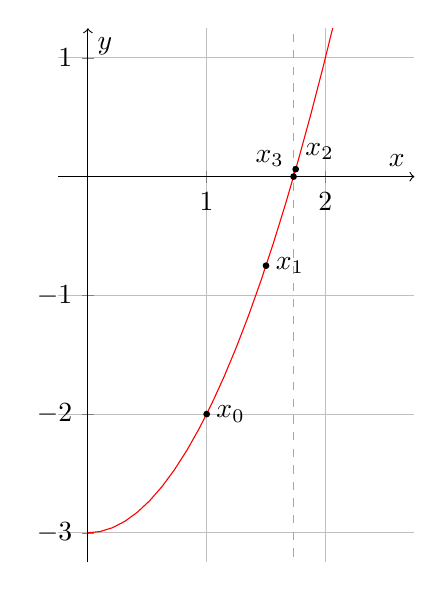
\begin{tikzpicture}
            \begin{axis}[
                    % xtick distance=2,
                    % ytick distance=2,
                    grid=major,
                    % grid style={line width=.1pt, draw=gray!10}%,major grid style={line width=.2pt,draw=gray!50}
                    % ticks=none, % ticks aus?
                    axis lines = middle,
                    axis line style={->},
                    ymin=-3.25, ymax=1.25,
                    xmin=-0.25, xmax=2.75,
                    xlabel={$x$},
                    ylabel={$y$},
                    axis equal image,
                    width=0.8\textwidth,
                    domain=0:2.5,
                ]
                % f = x^2-3
                \addplot[no marks, red]{x^2-3};
                \draw[red!50, dashed] (axis cs:1.73205,-3.2) -- (axis cs:1.73205,1.2);
                
                \draw[fill, black] (axis cs: 1, 1^2-3) circle (1pt) node[right] {$x_{0}$};
                \draw[fill, black] (axis cs: 1.5, 1.5^2-3) circle (1pt) node[right] {$x_{1}$};
                \draw[fill, black] (axis cs: 1.75, 1.75^2-3) circle (1pt) node[above right] {$x_{2}$};
                \draw[fill, black] (axis cs: 1.7321, 1.7321^2-3) circle (1pt) node[above left] {$x_{3}$};
            \end{axis}
        \end{tikzpicture}
    \end{center}
\end{example}

\begin{bonus}{Newton-Verfahren (Parabel)}
    Brechen wir nach dem quadratischen Term ab so folgt
    \[
        0 = f(x_k) + (\tilde{x} - x_k) f'(x_k) + \frac{(\tilde{x} - x_k)^2}{2} f''(x_k)
    \]
    und damit
    \[
        x_{k+1} = x_k - \frac{f'(x_k) \pm \sqrt{(f'(x_k))^2 - 2 \cdot f(x_k) f''(x_k)}}{f''(x_k)}
    \]
    
    Hier wird statt einer Tangente eine Parabel $g$ verwendet.
\end{bonus}

\subsection{Stationäre Iterationen, Banachscher Fixpunktsatz}

% \begin{defi}{Picard-Iteration}
%     TODO
% \end{defi}

\begin{defi}{Kontraktion}
    $\Phi$ heißt \emph{Kontraktion} bezüglich $\| \cdot \|$ auf $X \subset \R^n$ falls
    \begin{enumerate}
        \item $\Phi: X \to X$
        \item $\|\Phi(x) - \Phi(y)\| \leq \alpha \|x-y\|$, $\forall x, y \in X$ und $\alpha < 1$ unabhängig von $x, y$\footnote{Äquivalent: $\displaystyle \alpha \leq \max_{\zeta \in X} |\Phi'(\zeta)|$}
    \end{enumerate}
\end{defi}

\begin{example}{Kontraktion}
    Gegeben sei die Funktion $f(x) = x - e^{-x}$. 
    
    Zeigen Sie, dass das Newton-Verfahren $\Phi$ auf dem Intervall $X = [0, 1]$ konvergiert bzw. dass $\Phi$ eine Kontraktion auf $X$ ist.
    
    \exampleseparator
    
    Es gilt: 
    \[ 
        \Phi(x) = x - \frac{f(x)}{f'(x)} = x - \frac{x - e^{-x}}{1 + e^{-x}} = x - \frac{e^x \left(x - e^{-x}\right)}{e^x \left(1 + e^{-x}\right)} = \frac{x}{e^x + 1} - \frac{e^xx - 1}{e^x + 1} = \frac{x+1}{e^x + 1}
    \]
    
    $\Phi(x)$ ist eine Kontraktion, wenn: 
    \begin{itemize}
        \item $\Phi(x) \subset X \quad \iff \quad \forall x \in [0, 1]: \Phi(x) \in [0, 1]$:
              \begin{itemize}
                  \item Rand:
                        \[ \Phi(0) = \frac{1}{2} \in [0, 1], \quad \Phi(1) = \frac{2}{e + 1} \approx 0.5379 \in [0, 1] \]
                  \item lokale Extrema ($\Phi'(x) = 0$):
                        \[ 
                            \Phi(x) = x - \frac{f(x)}{f'(x)} \quad \implies \quad \Phi'(x) = \frac{f(x) f''(x)}{f'(x)}
                        \]
                        \[ 
                            \Phi'(x) = 0 \quad \iff \quad f(x) = 0 \quad \lor \quad \underbrace{f''(x) = 0}_{f''(x) = -e^{-x} \neq 0}
                        \]
                        \[ 
                            f(x) = 0 \quad \implies \quad \Phi(x) = x - \frac{0}{f'(x)} = x \in [0, 1]
                        \]
              \end{itemize}
        \item $\displaystyle \alpha \leq \max_{\zeta \in X} |\Phi'(\zeta)|$:
              \[ 
                  \Phi'(\zeta) = \left(\frac{\zeta+1}{e^\zeta + 1}\right)' = \frac{e^\zeta + 1 - (\zeta + 1) e^\zeta}{(e^\zeta + 1)^2} = \frac{1 - \zeta e^\zeta}{(e^\zeta + 1)^2}
              \]
              \[ 
                  \max_{\zeta \in X} |\Phi'(\zeta)| = \max_{\zeta \in [0, 1]} \frac{|1 - \zeta e^\zeta|}{(e^\zeta + 1)^2} \leq \frac{\displaystyle \max_{\zeta \in [0, 1]} |1 - \zeta e^\zeta|}{\displaystyle \min_{\zeta \in [0, 1]} (e^\zeta + 1)^2}
              \]
              \[ 
                  \displaystyle \min_{\zeta \in [0, 1]} (e^\zeta + 1)^2 = (1 + 1)^2 = 4
              \]
              \[ 
                  \displaystyle \max_{\zeta \in [0, 1]} |\underbrace{1 - \zeta e^\zeta}_{\text{mon. fall.}}| = \max \left\{ |1 - \zeta e^0|, |1 - \zeta e^1| \right\} = \max \left\{ 1, e-1 \right\} = e-1
              \]
              \[ 
                  \implies \alpha \leq \frac{e-1}{4} \approx \frac{1.718}{4} < \frac{1}{2}
              \]
              \qed
    \end{itemize}
\end{example}

\begin{defi}{Lokale Konvergenz (Iterationen)}
    Die Iteration
    \[
        x_{k+1} = \Phi(x_k)
    \]
    heißt \emph{lokal konvergent} gegen $x \in X \subset \R^n$ falls
    \[
        \lim_{k \to \infty} x_k = x \quad \forall x_0 \in X
    \]
\end{defi}

\begin{defi}{Banachscher Fixpunktsatz}
    Sei $X \subset \R^n$ abgeschlossen und $\Phi: X \to X$ eine Kontraktion auf $X$ mit
    \[
        \|\Phi(x) - \Phi(y)\| \leq \alpha \|x-y\| \quad x, y \in X, \alpha < 1
    \]
    
    Dann hat $\Phi$ genau einen Fixpunkt mit $x = \Phi(x)$ in $X$.
    
    Die Picard-Iteration
    \[
        x_{k+1} = \Phi(x_k)
    \]
    konvergiert $\forall x_0 \in X$ gegen $x$.
    Es gelten die Abschätzungen
    \[
        \|e_k\| = \|x - x_k\| \leq \frac{\alpha^k}{1-\alpha} \|x_1 - x_0\| \qquad \text{\emph{a-priori Abschätzung}}
    \]
    \begin{itemize}
        \item $\|e_k\|$ kann allein mit $\alpha, x_0, x_1$ abgeschätzt werden, ohne Ausrechnen von $x_k$
        \item wird benutzt um maximale Zahl der Iterationen für gegebene Genauigkeit zu bestimmen
        \item oft sehr grob
    \end{itemize}
    
    \[
        \|e_k\| = \|x - x_k\| \leq \frac{\alpha}{1-\alpha} \|x_k - x_{k-1}\| \qquad \text{\emph{a-posteriori Abschätzung}}
    \]
    \begin{itemize}
        \item $\|e_k\|$ kann mit $\alpha, x_k, x_{k-1}$ erst abgeschätzt werden, wenn $x_k$ berechnet wurde
        \item in der Regel genauer als a-priori Abschätzung
        \item oft als Abbruchkriterium genutzt
    \end{itemize}
    
    Es gilt:
    \begin{itemize}
        \item ist $\Phi$ eine Kontraktion, so existiert genau ein Fixpunkt
        \item $x_k$ konvergiert gegen $x$
        \item Kontraktion $\implies$ Konvergenz
        \item in der Regel erhält man nur lokale Konvergenz ($X \neq \R^n$)
        \item Banach liefert nur hinreichende, keine notwendigen Konvergenzkriterien
    \end{itemize}
\end{defi}


\begin{example}{Banachscher Fixpunktsatz}
    Gegeben sei die Funktion $f(x) = x^2 - 2$. 
    
    Zeigen Sie auch, dass $\Phi(x)$ eine Kontraktion auf $X = [1, 2]$ ist.
    
    Bestimmen Sie nach dem Banachschen Fixpunktsatz die Abschätzungen für das Newton-Verfahren für $f(x)$. 
    
    \exampleseparator
    
    Die Iteration des Newton-Verfahren ist bekanntermaßen gegeben mit:
    \[ 
        \Phi(x) = x - \frac{f(x)}{f'(x)} = x - \frac{2x^2 - 2}{2x} = \frac{x}{2} + \frac{1}{x}
    \]
    
    Die Fixpunkte sind dann: 
    \[ 
        x = \Phi(x) \quad \iff \quad x = \frac{x}{2} + \frac{1}{x} \quad \iff \quad \frac{x}{2} = \frac{1}{x} \quad \iff \quad x^2 = 2 \quad \iff \quad x = \pm \sqrt{2}
    \]
    
    Kontraktion: 
    \begin{itemize}
        \item $\Phi(x) \subset X$, denn für $y \in [1, 2]$ ist $\Phi(y)$ monoton und es gilt:
              \[ 
                  \Phi(y) = \frac{y}{2} + \frac{1}{y} \geq \frac{1}{2} + \frac{1}{2} = 1 \quad \implies \quad \Phi(x) \in \left[1, \infty\right)
              \]
              \[ 
                  \Phi(y) = \frac{y}{2} + \frac{1}{y} \leq \frac{2}{2} + \frac{1}{1} = 2 \quad \implies \quad \Phi(x) \in \left[1, 2\right]
              \]
        \item $|\Phi(x) - \Phi(y)\ \leq \alpha |x-y|$, $\forall x, y \in X$:
              
              $\Phi$ ist auf $X$ differenzierbar mit $\Phi'(y) = \frac{1}{2} - \frac{1}{y^2}$, so dass für alle $\zeta \in X$ gilt: 
              \[ 
                  \Phi'(\zeta) = \frac{1}{2} - \frac{1}{\zeta^2} \geq \frac{1}{2} - \frac{1}{1} \geq -\frac{1}{2} \implies \quad \Phi'(x) \in \left[-\frac{1}{2}, \infty\right)
              \]
              \[ 
                  \Phi'(\zeta) = \frac{1}{2} - \frac{1}{\zeta^2} \leq \frac{1}{2} - \frac{1}{2} \leq \frac{1}{4} \quad \implies \quad \Phi'(x) \in \left[-\frac{1}{2}, \frac{1}{4}\right]
              \]
              
              Damit gilt: 
              \[ 
                  |\Phi(x) - \Phi(y)| = |\Phi'(\zeta)| \cdot |x - y| \leq \frac{1}{2} |x-y| = \alpha |x-y|, \quad \forall x, y \in X = [1, 2]
              \]
    \end{itemize}
    
    Damit ist $\Phi$ eine Kontraktion auf $X$ mit $\alpha = \nicefrac{1}{2}$ und $\Phi$ hat genau einen Fixpunkt auf $X$.
    
    Dann gilt für die \emph{a-priori Abschätzung}: 
    \[ 
        |e_k| = |x - x_k| \leq \frac{\alpha^k}{1-\alpha} |x_1 - x_0| = \left(\frac{1}{2}\right)^{k-1} |x_1 - x_0|
    \]
    
    Und für die \emph{a-posteriori Abschätzung}:
    \[ 
        |e_k| = |x - x_k| \leq \frac{\alpha}{1-\alpha} |x_k - x_{k-1}| = |x_k - x_{k-1}|
    \]
\end{example}

\begin{defi}{Konvergenzgeschwindigkeit}
    \index{Lineare Konvergenz}
    \index{Konvergenzordnung}
    \index{a-priori Abschätzung}
    \index{a-posteriori Abschätzung}
    %
    Die Iteration $x_{k+1} = \Phi(x_k)$ heißt
    \begin{itemize}
        \item \emph{linear konvergent}, falls es eine Konstante $0 \leq c < 1$ unabhängig von $k$ gibt mit
              \[
                  \|e_{k+1}\| \leq c \|e_k\| \quad \forall k
              \]
        \item \emph{konvergent mit Ordnung} $m$, falls es eine Konstante $0 \leq c$ unabhängig von $k$ gibt mit
              \[
                  \lim_{k \to \infty} \|e_k\| = 0 \quad \land \quad \|e_{k+1}\| \leq c \|e_k\|^m \quad \forall k
              \]
              \begin{itemize}
                  \item Ist $m > 1$, so nennt man $\Phi$ \emph{superlinear konvergent}.
                  \item Für $m = 2$ erhalten wir \emph{quadratische Konvergenz}.
              \end{itemize}
    \end{itemize}
\end{defi}

\begin{bonus}{Konvergenzgeschwindigkeit stetig differenzierbarer Funktionen I}
    Ist $m \geq 2$, $x$ ein Fixpunkt von $\Phi: \R \to \R$ und $\Phi$ $m$-mal stetig differenzierbar in $x$ mit
    \[
        \Phi'(x) = \Phi''(x) = \cdots = \Phi^{(m-1)}(x) = 0
    \]
    dann gibt es ein abgeschlossenes Intervall $X = [ x - \delta, x + \delta ]$, $\delta > 0$, so dass die Iteration
    \[
        x_{k+1} = \Phi(x_k)
    \]
    für alle $x_0 \in X$ \emph{mindestens mit Ordnung $m$ konvergiert}.
\end{bonus}

\begin{bonus}{Konvergenzgeschwindigkeit stetig differenzierbarer Funktionen II}
    Ist $m \geq 2$, $x$ ein Fixpunkt von $\Phi: \R \to \R$ und $\Phi$ $(m-1)$-mal stetig differenzierbar in $x$ mit
    \[
        \Phi'(x) = \Phi''(x) = \cdots = \Phi^{(m-1)}(x) = 0, \quad \Phi^{(m)} \neq 0
    \]
    dann gibt es ein abgeschlossenes Intervall $X = [ x - \delta, x + \delta ]$, $\delta > 0$, so dass die Iteration
    \[
        x_{k+1} = \Phi(x_k)
    \]
    für alle $x_0 \in X$ \emph{genau mit Ordnung $m$ konvergiert}.
\end{bonus}

\begin{bonus}{Konvergenzgeschwindigkeiten relevanter Verfahren}
    \begin{itemize}
        \item Das Bisektions-Verfahren ist linear konvergent mit $c = \nicefrac{1}{2}$.
        \item Das Regula-Falsi-Verfahren ist linear konvergent.
        \item Das Sekanten-Verfahren hat die Konvergenzordnung $m = \frac{1 + \sqrt{5}}{2} \approx 1.618$.
    \end{itemize}
\end{bonus}

\subsection{Newton-Verfahren}

\begin{defi}{Konvergenzgeschwindigkeit des Newton-Verfahrens (einfache Nullstellen)}
    $f: \R \to \R$ sei zweimal stetig differenzierbar mit $f(x) = 0$, $f'(x) \neq 0$, d. h. $x$ ist eine \emph{einfache Nullstelle} von $f$. 
    
    Liegt $x_0$ nahe genug an $x$, dann konvergiert das Newton-Verfahren \emph{quadratisch} gegen $x$.
\end{defi}

\begin{defi}{Konvergenzgeschwindigkeit des Newton-Verfahrens (mehrfache Nullstellen)}
    Für \emph{mehrfache Nullstellen} ist das Newton-Verfahren wohldefiniert und konvergiert nur \emph{linear} in einer Umgebung von $x$.
    
    Verbesserte Variante 1: 
    \begin{itemize}
        \item Setze
              \[ 
                  \tilde{\Phi}(y) = y - q \cdot \frac{f(y)}{f'(y)}
              \]
              und iteriere 
              \[
                  x_{k-1} = \tilde{\Phi}(x_k)
              \]
        \item Durch Ausrechnen erhält man $\tilde{\Phi}(x) = 0$ und damit (mind.) quadratische Konvergenz.
        \item Nachteil: Vielfachheit von $q$ muss bekannt sein.
    \end{itemize}
    
    Verbesserte Variante 2:
    \begin{itemize}
        \item $x$ ist $q$-fache Nullstelle, daher erhalten wir aus einer Taylorentwicklung von $f$
              \[ 
                  f(y) = \frac{1}{q!} (y - x)^q f^{(q)} (\zeta), \quad f'(y) = \frac{1}{(q-1)!} (y - x)^{q-1} f^{(q)} (\eta)
              \]
        \item Da $f^{(q)} (x) \neq 0$ ist, folgt für $y$ nahe $x$, dass $f^{(q)} (\zeta) \neq 0$ und $f^{(q)} (\eta) \neq 0$ und damit
              \[ 
                  \tilde{f} (y) = \frac{f(y)}{f'(y)} = \frac{\frac{1}{q!} (y - x)^q f^{(q)} (\zeta)}{\frac{1}{(q-1)!} (y - x)^{q-1} f^{(q)} (\eta)} = \frac{1}{q} \cdot (y - x) \cdot \frac{f^{(q)} (\zeta)}{f^{(q)} (\eta)}
              \]
              d. h. $x$ ist einfache Nullstelle von $\tilde{f} = \frac{f}{f'}$
        \item wird das Newton-Verfahren auf $\tilde{f}$ angewandt, konvergiert es quadratisch
        \item Vielfachheit $q$ wird hier nicht explizit benutzt
        \item Nachteil: komplizierte Iterationsvorschrift:
              \[
                  \Phi(y) = y - \frac{\tilde{f}(y)}{\tilde{f}'(y)} = \ldots = y - \frac{f(y) f'(y)}{\left( f'(y) \right)^2 - f(y) f''(y)}
              \]
              in der pro Schritt neben $f$ und $f'$ auch noch $f''$ auszuwerten ist.
    \end{itemize}
\end{defi}

\begin{defi}{Newton-Verfahren (mehrdimensional)}
    Für ein $f: \R \to \R$ erhalten wir die Taylorentwicklung 
    \[
        f(y) = f(x_k) + J(x_k) (y - x_k) + R
    \]
    mit der Jacobi-Matrix $J$ von $f$ in $x_k$
    \[
        J = \begin{pmatrix}
            \partial_1 f_1 (x_k) & \cdots & \partial_n f_1 (x_k)  \\ 
            \vdots               &        & \vdots                \\ 
            \partial_1 f_n (x_k) & \cdots & \partial_n f_n (x_k) 
        \end{pmatrix}
    \]
    
    Dann gilt für reguläres $J(x_k)$ direkt\footnote{Eine reguläre Jacobi-Matrix entspricht einer einfachen Nullstelle im eindimensionalen Fall.}
    \[
        x_{k+1} = x_k - \left( J(x_k) \right)^{-1} f(x_k)    
    \]
    
    In diesem Fall konvergiert das Newton-Verfahren quadratisch.
    
    Die Behandlung für eine singuläre Jacobi-Matrix ist etwas komplizierter als im skalaren Fall.\footnote{Eine singuläre Jacobi-Matrix entspricht einer mehrfachen Nullstelle im eindimensionalen Fall.}
\end{defi}
\section{Interpolation}

\subsection{Einleitung}

\begin{defi}{Interpolation}
    Der Begriff \emph{Interpolation} bescheibt eine Klasse von Problemen und Verfahren. 
    
    Zu gegebenen diskreten Daten (z. B. Messwerten) soll eine stetige Funktion (die sogenannte \emph{Interpolante} oder \emph{Interpolierende}) gefunden werden, die diese Daten abbildet. 
    
    Man sagt dann, die Funktion \emph{interpoliert} die Daten. 
\end{defi}

\subsection{Polynominterpolation}

\begin{defi}{Vandermonde-Matrix}
    Die \emph{Vandermonde-Matrix} spielt bei der Interpolation von Funktionen eine wichtige Rolle: 
    
    Wenn an den Stützstellen $(x_0, x_1, \ldots, x_n)$ die Funktionswerte $(y_0, y_1, \ldots, y_n)$ durch ein Polynom $p$ vom Grad $n$ (oder kleiner) interpoliert werden sollen, dann führt der Ansatz 
    \[
        p_n(x) = a_0 + a_1 x^1 + a_2 x^2 + \ldots + a_{n} x^{n}
    \]
    auf das lineare Gleichungssystem 
    \[
        \underbrace{\begin{pmatrix}
                1      & x_0    & \cdots & x_0^n  \\ 
                \vdots & \vdots &        & \vdots \\ 
                1      & x_n    & \cdots & x_n^n 
            \end{pmatrix}}_{V(x_0, \ldots, x_n)}
        \underbrace{\begin{pmatrix}
                a_0 \\ \vdots \\ a_n
            \end{pmatrix}}_{\alpha}
        =
        \underbrace{\begin{pmatrix}
                y_0 \\ \vdots \\ y_n     
            \end{pmatrix}}_{y}
    \]
    mit einer Vandermonde-Matrix $Vx_0, \ldots, x_n)$ als Koeffizientenmatrix.\footnote{Beachte: Für ein Polynom vom Grad $n$ haben wir $n+1$ Koeffizienten!}
    
    Ist $x_i \neq x_j$ ($\forall i \neq j$) so gibt es genau ein Polynom $p_n(x)$ mit Grad $\leq n$, das $(x_0, y_0), \ldots, (x_n, y_n)$ interpoliert. 
\end{defi}

\begin{defi}{Vandermonde-Determinante}
    Die Determinante der Vandermonde-Matrix wird auch \emph{Vandermonde-Determinante} genannt.
    Sie hat den Wert 
    \[
        \det V(x_0, \ldots, x_n) = \prod_{1 \leq i < j \leq n} (x_j - x_i)
    \]
    
    Insbesondere ist die Vandermonde-Matrix genau dann regulär, wenn die $x_i$ paarweise verschieden sind. 
\end{defi}

\begin{defi}{Horner-Schema}
    Um Zwischenstellen eines Polynoms $p_n(x)$ auszuwerten, nutzt man in der Regel nicht direkt die Form 
    \[
        p_n(x) = a_0 + a_1 x + \ldots + a_n x^n    
    \]
    Diese Auswertung ist teuer und durch die vielen Summationen sehr anfällig für Rundungsfehler.
    
    Besser ist hier das \emph{Horner-Schema}: 
    \begin{itemize}
        \item $p_n(x)$ wird wie folgt umgeformt:
              \begin{alignat*}{1}
                  p_n (x) & = a_0 + a_1 x + a_2 x^2 + \ldots + a_n x^n                                                                                                                                                      \\ 
                          & = a_0 + x \left( a_1 + a_2 x + \ldots + a_n x^{n-1} \right)                                                                                                                                     \\ 
                          & = a_0 + x \left( a_1 + x \left( a_2 + \ldots + a_n x^{n-2} \right) \right)                                                                                                                      \\ 
                          & = \ \ldots                                                                                                                                                                                      \\ 
                          & = \underbrace{a_0 + x \underbrace{( a_1 + x \underbrace{( a_2 + x \underbrace{( \ldots + x \underbrace{( a_{n-1} + x \underbrace{a_n}_{q_0} )}_{q_1} )}_{\ldots} )}_{q_{n-2}} )}_{q_n-1}}_{q_n}
              \end{alignat*}
        \item Berechne schrittweise von innen nach außen:
              \begin{alignat*}{1}
                  q_0 & = a_n                   \\ 
                  q_1 & = a_{n-1} + x \cdot q_0 \\
                  q_2 & = a_{n-2} + x \cdot q_1 \\
                      & \ldots
              \end{alignat*}
              also
              \[ 
                  q_0 = a_n, \quad q_k = a_{n-k} + x \cdot q_{k-1}, \quad k = 1, \ldots, n
              \]
              und damit 
              \[ 
                  p_n(x) = q_n
              \]
    \end{itemize}
\end{defi}

\begin{defi}{Lagrange-Polynom}
    Wir betrachten $x_0, \ldots, x_n$ und definieren das $j$-te \emph{Lagrange-Polynom} als 
    \[ 
        L_j(x) = \frac{x - x_0}{x_j - x_0} \cdot \frac{x - x_{j-1}}{x_j - x_{j-1}} \cdot \frac{x - x_{j+1}}{x_j - x_{j+1}} \cdot \ldots \cdot \frac{x - x_n}{x_j - x_n}
    \]
    
    $L_j$ ist wohldefiniert, wenn die $x_i$ paarweise verschieden sind und hat Grad $n$.
    
    Außerdem gilt 
    \[
        L_j(x_i) = 
        \begin{cases}
            1 & \text{für} \ i = j \\ 
            0 & \text{sonst}
        \end{cases}
    \]
    
    Mit den Lagrange-Polynomen $L_j$ können wir das Interpolationspolynom einfach ermitteln mit 
    \[
        p_n(x) = \sum_{j = 0}^{n} y_j \cdot L_j(x)    
    \]
    
    Bei der Benutzung der Lagrange-Polynome muss kein Gleichungssystem gelöst werden, allerdings müssen sämtliche $L_j$ verändert werden, wenn ein weiterer Datenpunkt hinzukommt.
\end{defi}

\begin{example}{Lagrange-Polynom}
    Gegeben seien die folgenden Datenpunkte: 
    
    \begin{center}
        \begin{tabular}{|c||c|c|c|c|}
            \hline
            $x_i$ & -1 & 0 & 1 & 2 \\ 
            \hline
            $y_i$ & 2  & 2 & 2 & 8 \\
            \hline
        \end{tabular}
    \end{center}
    
    Berechnen Sie das zugehörige Lagrange-Interpolationspolynom.
    
    \exampleseparator
    
    Die Lagrange-Polynome sind wie folgt: 
    \[ 
        L_0(x) = \frac{x - x_1}{x_0 - x_1} \cdot \frac{x - x_2}{x_0 - x_2} \cdot \frac{x - x_3}{x_0 - x_3} = \frac{x - 0}{-1 - 0} \cdot \frac{x - 1}{-1 - 1} \cdot \frac{x - 2}{-1 - 2} = -\frac{x(x-1)(x-2)}{6}
    \]
    \[ 
        L_1(x) = \frac{x - x_0}{x_1 - x_0} \cdot \frac{x - x_2}{x_1 - x_2} \cdot \frac{x - x_3}{x_1 - x_3} = \frac{x - (-1)}{0 - (-1)} \cdot \frac{x - 1}{0 - 1} \cdot \frac{x - 2}{0 - 2} = \frac{(x+1)(x-1)(x-2)}{2}
    \]
    \[ 
        L_2(x) = \frac{x - x_0}{x_2 - x_0} \cdot \frac{x - x_1}{x_2 - x_1} \cdot \frac{x - x_3}{x_2 - x_3} = \frac{x - (-1)}{1 - (-1)} \cdot \frac{x - 0}{1 - 0} \cdot \frac{x - 2}{1 - 2} = -\frac{(x+1)x(x-2)}{2}
    \]
    \[ 
        L_3(x) = \frac{x - x_0}{x_3 - x_0} \cdot \frac{x - x_1}{x_3 - x_1} \cdot \frac{x - x_2}{x_3 - x_2} = \frac{x - (-1)}{2 - (-1)} \cdot \frac{x - 0}{2 - 0} \cdot \frac{x - 1}{2 - 1} = \frac{(x+1)x(x-2)}{6}
    \]
    
    Damit ist das Lagrange-Interpolationspolynom $p(x)$: 
    \begin{alignat*}{1}
        p(x) = \quad & y_0 L_0 + y_1 L_1 + y_2 L_2 + y_3 L_3                                                                  \\
        =      \quad & -\frac{2x(x-1)(x-2)}{6} + \frac{2(x+1)(x-1)(x-2)}{2} - \frac{2(x+1)x(x-2)}{2} + \frac{8(x+1)x(x-2)}{6} \\ 
        =      \quad & \ldots                                                                                                 \\ 
        =      \quad & x^3 - x + 2
    \end{alignat*}
\end{example}

\begin{defi}{Newton-Interpolationspolynom}
    \index{Methode der dividierten Differenzen}
    %
    Ein \emph{Newton-Interpolationspolynom} ist ein Interpolationspolynom für eine bestimmte Menge von Datenpunkten.
    
    Gegeben seien $n+1$ paarweise verschiedene Datenpunkte $(x_0, y_0), \ldots, (x_n, y_n)$.
    
    Das \emph{Newton-Interpolationspolynom} ist dann eine Linearkombination der Newton-Basispolynome $N_j(x)$ mit 
    \[ 
        p_n(x) = \sum_{j=0}^{n} a_j N_j(x)  
    \]
    \[  
        = a_0 + a_1 (x - x_0) + a_2 (x - x_0) (x - x_1) + \ldots + a_n (x - x_0) \cdot \ldots \cdot (x - x_{n-1})
    \]
    wobei 
    \[
        N_j (x) = \prod_{i=0}^{j-1} \left( x - x_i \right)
    \]
    
    Die $a_j$ lassen sich wie folgt mithilfe der \emph{Methode der dividierten Differenzen} berechnen.
    
    Es gilt 
    \[ 
        a_j = d_{n, 0}, \quad j = 0, \ldots, n
    \]
    
    Dabei ist 
    \[ 
        d_{n, m} = \frac{d_{n, m+1} - d_{n-1, m}}{x_n - x_m}, \quad n > m
    \]
    mit 
    \[
        d_{i,i} = y_i, \quad i = 0, 1, \ldots    
    \]
    
    Bei gegebenen Punkten $(x_i, y_i)$ kann damit punktweise (Zeile für Zeile) folgendes Schema aufgebaut werden:
    \[
        \begin{array}{cccccccccccccc}
            y_0     & = & d_{0,0}      & =           & a_0                                                                                                              \\
                    &   &              & \searrow                                                                                                                       \\
            y_1     & = & d_{1,1}      & \rightarrow & d_{1,0}      & =           & a_1                                                                                 \\
                    &   &              & \searrow    &              & \searrow                                                                                          \\
            y_2     & = & d_{2,2}      & \rightarrow & d_{2,1}      & \rightarrow & d_{2,0}      & =      & a_2                                                         \\
            \vdots  &   &              & \vdots      & \vdots       & \vdots      & \vdots       & \ddots                                                               \\
            y_{n-1} & = & d_{n-1, n-1} & \rightarrow & d_{n-1, n-2} & \rightarrow & d_{n-1, n-3} & \cdots & \rightarrow & d_{n-1, 0} & =           & a_{n-1}            \\
                    &   &              & \searrow    &              & \searrow    &              &        & \searrow    &            & \searrow                         \\
            y_n     & = & d_{n,n}      & \rightarrow & d_{n, n-1}   & \rightarrow & d_{n, n-2}   & \cdots & \rightarrow & d_{n, 1}   & \rightarrow & d_{n, 0} & = & a_n
        \end{array}
    \]
    
    Wird ein Punkt hinzugefügt, wird das Schema lediglich um eine Zeile erweitert.
    
    Insgesamt ist das Newton-Interpolationspolynom also gegeben mit 
    \[ 
        p_n(x) = \sum_{j=0}^{n} d_{j,0} N_j(x)  
    \]
    \[  
        = d_{0, 0} + d_{1, 0} (x - x_0) + d_{2, 0} (x - x_0) (x - x_1) + \ldots + d_{n, 0} (x - x_0) \cdot \ldots \cdot (x - x_{n-1})
    \]
\end{defi}

\begin{example}{Newton-Interpolationspolynom}
    Gegeben seien die folgenden Datenpunkte: 
    
    \begin{center}
        \begin{tabular}{|c||c|c|c|c|}
            \hline
            $x_i$ & -1 & 0 & 1 & 2 \\ 
            \hline
            $y_i$ & 2  & 2 & 2 & 8 \\
            \hline
        \end{tabular}
    \end{center}
    
    Berechnen Sie das zugehörige Newton-Interpolationspolynom.
    
    \exampleseparator
    
    Das Newton-Interpolationspolynom ist:
    \[ 
        p_3(x) = \sum_{j=0}^{3} d_{j,0} N_j(x) 
    \]
    \[ 
        = a_0 + a_1 (x - x_0) + a_2 (x - x_0) (x - x_1) + a_3 (x - x_0) (x - x_1) (x - x_2) 
    \]
    
    Es gilt:
    
    {
    \footnotesize
    \[
        \begin{array}{llllllllllll}
            y_0 & = & d_{0,0} = 2 & =           & a_0                                                                                                                                                                                                              \\
                &   &             & \searrow                                                                                                                                                                                                                       \\
            y_1 & = & d_{1,1} = 2 & \rightarrow & d_{1,0} = \frac{d_{1,1} - d_{0,0}}{x_1 - x_0} = \frac{2 - 2}{0 + 1} = 0 & =           & a_1                                                                                                                      \\
                &   &             & \searrow    &                                                                         & \searrow                                                                                                                               \\
            y_2 & = & d_{2,2} = 2 & \rightarrow & d_{2,1} = \frac{d_{2,2} - d_{1,1}}{x_2 - x_1} = \frac{2 - 2}{1 - 0} = 0 & \rightarrow & d_{2,0} = \frac{d_{2,1} - d_{1,0}}{x_2 - x_0} = \frac{0 - 0}{1 + 1} = 0  & =           & a_2                             \\
                &   &             & \searrow    &                                                                         & \searrow    &                                                                          & \searrow                                      \\
            y_3 & = & d_{3,3} = 8 & \rightarrow & d_{3,2} = \frac{d_{3,3} - d_{2,2}}{x_3 - x_2} = \frac{8 - 2}{2 - 1} = 6 & \rightarrow & d_{3, 1} = \frac{d_{3,2} - d_{2,1}}{x_3 - x_1} = \frac{6 - 0}{2 - 0} = 3 & \rightarrow & d_{3, 0} = \ldots = 1 & = & a_3 \\
        \end{array}
    \]
    }
    
    Damit ist: 
    \[ 
        p_3(x) = 2 + 1 (x - x_0) (x - x_1) (x - x_2) = 2 + (x+1) x (x-1) = 2 + x(x^2 - 1) = 2 - x + x^3
    \]
    \qed
\end{example}

\subsection{Splines}

\begin{defi}{Polynom-Spline}
    Gegeben seien eine natürliche Zahl $n \in \N$ und $n+1$ Stützstellen $x_0 < x_1 < \ldots < x_{n} \in \R$ sowie $n+1$ Funktionswerte $y_0, y_1, \ldots, y_n \in \R$. 
    
    Gesucht ist eine stückweise polynomiale Funktion, ein \emph{Polynom-Spline}
    \[ 
        S: [x_0, x_n] \to \R
    \]
    mit $S(x_i) = y_i$ für $i = 0, 1, \ldots, n-1$, bei der für $i = 0, \ldots, n-1$ die Teilfunktionen 
    \[
        s_i := S|_{[x_{i},x_{i+1}]} : [x_i, x_{i+1}] \to \R
    \]
    auf die Teilintervalle $[x_{i}, x_{i+1}]$ Polynome sind.
\end{defi}

\begin{bonus}{Polygonzug}
    Bei Polynomgrad $\leq 1$ auf $[x_i, x_{i+1}]$ und stetigen Übergängen erhalten wir einen interpolierenden \emph{Polygonzug}.
    
    TODO Grafik von Folie 495
    
    Es gilt: 
    \[ 
        s_i(x) = mx + b = \underbrace{\frac{y_{i+1} - y_i}{x_{i+1} - x_i}}_{= m} \cdot x + \underbrace{y_i - \frac{y_{i+1} - y_i}{x_{i+1} - x_i} \cdot x_i}_{= b = y_i - m \cdot x_i}
    \]
\end{bonus}

\begin{defi}{Kubischer Polynom-Spline}
    In der Praxis werden \emph{kubische Polynom-Splines} ($k = 3$) am häufigsten benutzt:
    \[ 
        s_i := S_3|_{[x_i, x_{i+1}]} = a_i + b_i x + c_i x^2 + d_i x^3
    \]
    
    $S_3$ ist zweimal stetig differenzierbar auf $[x_0, x_n]$, also insbesondere an den Nahtstellen $x_i$, $i = 1, \ldots, n-1$.
    
    Wir haben $n$ Intervalle $[x_i, x_{i+1}]$, $i = 0, \ldots, n-1$, so dass $4n$ Koeffizienten $a_i, b_i, c_i, d_i$ zu bestimmen sind für die $n$ Polynome $s_i$. 
    
    Für alle kubischen Polynom-Splines gelten folgende Bedingungsgleichungen: 
    \begin{itemize}
        \item $2n$ Bedingungen für die Interpolation:
              \begin{alignat*}{1}
                  s_0(x_0)         & = y_0     \\
                  s_0(x_1)         & = y_1     \\
                  s_1(x_1)         & = y_1     \\
                  s_1(x_2)         & = y_2     \\
                  s_2(x_2)         & = y_2     \\
                  \vdots           &           \\
                  s_{n-1}(x_{n-1}) & = y_{n-1} \\
                  s_{n-1}(x_n)     & = y_n     \\
              \end{alignat*}
        \item $n-1$ Glattheitsbedingungen für die erste Ableitung:
              \begin{alignat*}{1}
                  s'_0(x_1)         & = s'_1(x_1)         \\
                  s'_1(x_2)         & = s'_2(x_2)         \\
                  \vdots            &                     \\
                  s'_{n-2}(x_{n-1}) & = s'_{n-1}(x_{n-1}) \\
              \end{alignat*}
        \item $n-1$ Glattheitsbedingungen für die zweite Ableitung:
              \begin{alignat*}{1}
                  s''_0(x_1)         & = s''_1(x_1)         \\
                  s''_1(x_2)         & = s''_2(x_2)         \\
                  \vdots             &                      \\
                  s''_{n-2}(x_{n-1}) & = s''_{n-1}(x_{n-1}) \\
              \end{alignat*}
    \end{itemize}
    
    Damit haben wir $4n-2$ Gleichungen für $4n$ Unbekannte und brauchen zwei zusätzliche \emph{Abschlussbedingungen}.
\end{defi}

\begin{bonus}{Moment (Idee)}
    Die zweite Ableitung eines kubischen Splines $S_3$ ist ein linearer Spline (Polygonzug). 
    
    Dieser kann wie folgt berechnet werden: 
    \[ 
        s''_i = \frac{x_{i+1} - x}{h_i} \cdot \beta_i + \frac{x - x_i}{h_i} \cdot \beta_{i-1}, \quad h_i = x_{i+1} - x_i, \quad i = 1, \ldots, n-1
    \]
    
    $\beta_i$ sind die sogenannten \emph{Momente}, welche den Werten von $S''(x_i)$ an den Stützstellen entsprechen und noch zu berechnen sind. 
    
    Durch zweifache Integration entstehen aus diesen Gleichungen Polynome dritten Grades mit zwei Parametern $c_i$ und $d_i$ der Form: 
    \[ 
        \frac{1}{6} \left( \frac{(x_{i+1} - x)^3}{h_i} \cdot \beta_i + \frac{(x - x_i)^3}{h_i} \cdot \beta_{i+1} \right) + c_i \cdot (x - x_i) + d_i
    \]
    
    Um die Stetigkeitsbedingungen $s_i(x_i) = y_i$ und $s_i(x_{i+1}) = y_{i+1}$ zu erfüllen, wählen wir
    \[
        d_i = y_i - \frac{h_i^2}{6}, \quad c = \frac{y_{i+1} - y_i}{h_i} - \frac{h_i}{6} \cdot (\beta_{i+1} - \beta_i)
    \]
    
    So sind bereits die nullten und die zweiten Ableitungen der Einschränkungen $s_i$ an den Stützstellen korrekt.
    Die Momente sind so zu wählen, dass auch die ersten Ableitungen an den Stützstellen gleich sind. 
    
    Mit
    \[ 
        s'_i(x) = \frac{1}{2} \left( - \frac{(x_{i+1} - x)^2}{h_i} \cdot \beta_i + \frac{(x - x_i)^2}{h_i} \cdot \beta_{i+1} \right) + c_i 
    \]
    und 
    \[ 
        s'_i(x_i) = s'_{i-1}(x_i)    
    \]
    lassen sich folgende Gleichungen aufstellen: 
    \[
        \frac{h_{i-1}}{6} \cdot M_{i-1} + \frac{h_{i-1}+h_{i}}{3} \cdot \beta_{i} + \frac{h_{i}}{6} \cdot \beta_{i+1} = \frac{y_{i+1}-y_{i}}{h_{i}} - \frac{y_{i}-y_{i-1}}{h_{i-1}}
    \]
    
    Für $i = 0$ und $i = n$ fehlen zwei Gleichungen, die sich aus den \emph{Abschlussbedingungen} ergeben.
    
    Dieses lineare Gleichungssystem kann auch durch folgende, tridiagonale, streng diagonaldominante Matrix ausgedrückt werden: 
    \[
        \begin{pmatrix}
            \mu_{0}         & \lambda_{0}           &                   &                         &                  &          \\
            \frac{h_{0}}{6} & \frac{h_{0}+h_{1}}{3} & \frac {h_{1}}{6}  &                         &                  &          \\
                            & \ddots                & \ddots            & \ddots                  &                  &          \\
                            &                       & \frac{h_{i-1}}{6} & \frac{h_{i-1}+h_{i}}{3} & \frac {h_{i}}{6} &          \\
                            &                       &                   & \ddots                  & \ddots           & \ddots   \\
                            &                       &                   &                         & \lambda _{n}     & \mu _{n}
        \end{pmatrix}
        \cdot 
        \begin{pmatrix}
            M_{0} \\ M_{1} \\ \vdots \\ M_{i} \\ \vdots \\ M_{n}
        \end{pmatrix}
        =
        \begin{pmatrix}
            b_{0}                                                       \\
            \frac{y_{2}-y_{1}}{h_{1}} - \frac{y_{1}-y_{0}}{h_{0}}       \\
            \vdots                                                      \\
            \frac{y_{i+1}-y_{i}}{h_{i}} - \frac{y_{i}-y_{i-1}}{h_{i-1}} \\
            \vdots                                                      \\
            b_{n}
        \end{pmatrix}
    \]
    Die Werte für die $\lambda_i$, $\mu_i$ und $b_i$ hängen von den Abschlussbedingungen ab.
\end{bonus}

\begin{defi}{Berechnung eines kubischen Polynom-Splines}
    Berechne aus $x_i$ die $h_i = x_{i+1} - x_i$ und stelle das lineare Gleichungssystem 
    \[
        \underbrace{
            \begin{pmatrix}
                \mu_{0}         & \lambda_{0}           &                   &                         &                  &          \\
                \frac{h_{0}}{6} & \frac{h_{0}+h_{1}}{3} & \frac {h_{1}}{6}  &                         &                  &          \\
                                & \ddots                & \ddots            & \ddots                  &                  &          \\
                                &                       & \frac{h_{i-1}}{6} & \frac{h_{i-1}+h_{i}}{3} & \frac {h_{i}}{6} &          \\
                                &                       &                   & \ddots                  & \ddots           & \ddots   \\
                                &                       &                   &                         & \lambda _{n}     & \mu _{n}
            \end{pmatrix}
        }_{A}
        \cdot 
        \underbrace{
            \begin{pmatrix}
                M_{0} \\ M_{1} \\ \vdots \\ M_{i} \\ \vdots \\ M_{n}
            \end{pmatrix}
        }_{x}
        =
        \underbrace{
            \begin{pmatrix}
                b_{0}                                                       \\
                \frac{y_{2}-y_{1}}{h_{1}} - \frac{y_{1}-y_{0}}{h_{0}}       \\
                \vdots                                                      \\
                \frac{y_{i+1}-y_{i}}{h_{i}} - \frac{y_{i}-y_{i-1}}{h_{i-1}} \\
                \vdots                                                      \\
                b_{n}
            \end{pmatrix}
        }_{b}
    \]
    auf. 
    Die Werte für die $\lambda_i$, $\mu_i$ und $b_i$ hängen von den Abschlussbedingungen ab.\footnote{Wir betrachten meist \emph{natürliche Splines}, also $\lambda_0 = \lambda_n = b_0 = b_n = 0, \quad \mu_0 = \mu_n = 1$.}
    
    $A$ ist symmetrisch, tridiagonale und streng diagonaldominant, also sehr einfach mit direkten oder iterativen Lösern zu bearbeiten. 
    
    Löse das lineare Gleichungssystem.
    
    Dann ist $s_i(x)$ auf dem Teilintervall $[x_i, x_{i+1}]$ gegeben mit
    \[ 
        s_i(x) = \alpha_i + \beta_i (x - x_{i}) + \gamma_i (x - x_{i})^2 + \delta_i (x - x_{i})^3
    \]
    wobei
    \begin{alignat*}{1}
        \alpha_i & = y_i                                                        \\ 
        \beta_i  & = \frac{y_{i+1} - y_i}{h_i} - \frac{h_i}{6} (2M_i + M_{i+1}) \\
        \gamma_i & = \frac{M_{i}}{2}                                            \\ 
        \delta_i & = \frac{M_{i+1} - M_{i}}{6 h_i}
    \end{alignat*}
\end{defi}

\begin{defi}{Abschlussbedingungen für kubische Polynom-Splines}
    Prinzipiell gibt es ein Interpolationsintervall weniger als Stützstellen. 
    Das heißt, dass zwei Gleichungen zur Bestimmung aller Koeffizienten fehlen. 
    
    Typische \emph{Abschlussbedingungen} sind: 
    \begin{itemize}
        \item \emph{Natürlicher Spline} (freier Rand):
              \begin{itemize}
                  \item Bedingung:
                        \begin{alignat*}{1}
                            s''_0(x_0)     & = 0 \\
                            s''_{n-1}(x_n) & = 0
                        \end{alignat*}
                  \item Der Spline schließt mit Wendepunkten ab.
                  \item Berechnung mit Momenten:
                        \[
                            \lambda_0 = \lambda_n = b_0 = b_n = 0, \quad \mu_0 = \mu_n = 1
                        \]
              \end{itemize}
        \item \emph{Hermiter Spline} (eingespannter Rand):
              \begin{itemize}
                  \item Bedingung:
                        \begin{alignat*}{1}
                            s'_0(x_0)     & = f'(a) \\
                            s'_{n-1}(x_n) & = f'(b)
                        \end{alignat*}
                  \item $f'(a)$ und $f'(b)$ sind vorgegeben, normalerweise entweder durch die Ableitung einer zu interpolierenden Funktion $f$ oder durch eine Approximation derselben.
                  \item Berechnung mit Momenten:
                        \[
                            \lambda_0 = \frac{h_0}{6}, \quad \mu_0 = \frac{h_0}{3}, \quad b_0 = \frac{y_1 - y_0}{h_0} - f'(a)
                        \]
                        \[
                            \lambda_n = \frac{h_{n-1}}{6}, \quad \mu_n = \frac{h_{n-1}}{3}, \quad b_n = - \frac{y_n - y_{n-1}}{h_{n-1}} + f'(b)
                        \]
              \end{itemize}
        \item \emph{Periodischer Spline}:
              \begin{itemize}
                  \item Bedingung:
                        \begin{alignat*}{1}
                            s'_0(x_0)  & = s'_{n-1}(x_n)  \\
                            s''_0(x_0) & = s''_{n-1}(x_n) \\
                        \end{alignat*}
                  \item Nullte, erste und zweite Ableitung von $S_3$ am Anfang und Ende des Intervalls gleich.
                  \item Berechnung mit Momenten:
                        \[
                            \lambda_0 = \frac{h_0}{6}, \quad \mu_0 = \frac{h_n + h_0}{3}, \quad b_0 = \frac{y_1 - y_0}{h_0} - \frac{y_0 - y_n}{h_n}
                        \]
                        \[
                            \lambda_n = \frac{h_{n-1}}{6}, \quad \mu_n = \frac{h_{n-1} + h_n}{3}, \quad b_n = \frac{y_0 - y_n}{h_n} - \frac{y_n - y_{n-1}}{h_{n-1}}
                        \]
              \end{itemize}
    \end{itemize}
\end{defi}

\begin{example}{Kubischer Polynom-Spline (Bedingungsgleichungen)}
    Gegeben seien die folgenden Datenpunkte: 
    
    \begin{center}
        \begin{tabular}{|c||c|c|c|c|}
            \hline
            $x_i$ & -1 & 0 & 1 \\ 
            \hline
            $y_i$ & 1  & 0 & 1 \\
            \hline
        \end{tabular}
    \end{center}
    
    Berechnen Sie den zugehörigen kubischen Polynom-Spline mithilfe der Bedingungsgleichungen.
    
    \exampleseparator
    
    Wir wissen: 
    \[ 
        p(x) = a + bx + cx^2 + dx^3
    \]
    \[ 
        p'(x) = b + 2cx + 3dx^2
    \]
    \[ 
        p''(x) = 2c + 6dx
    \]
    
    Wir haben folgende Bedingungsgleichungen:
    \begin{alignat*}{3}
        \text{Interpolation:} \qquad              & p_L(x_0)       = y_0        \quad & \implies \quad & a_L - b_L + c_L - d_L =  1 \\
        \text{Interpolation:} \qquad              & p_L(x_1)       = y_1        \quad & \implies \quad & a_L =  0                   \\
        \text{Interpolation:} \qquad              & p_R(x_1)       = y_1        \quad & \implies \quad & a_R = 0                    \\
        \text{Interpolation:} \qquad              & p_R(x_2)       = y_2        \quad & \implies \quad & a_R + b_R + c_R + d_R = 1  \\
        \text{Glattheit erste Ableitung:} \qquad  & p'_L(x_1)      = p'_R(x_1)  \quad & \implies \quad & b_L = b_R                  \\
        \text{Glattheit zweite Ableitung:} \qquad & p''_L(x_1)     = p''_R(x_1) \quad & \implies \quad & 2c_L = 2c_R                \\
        \text{natürlicher Spline:} \qquad         & p''_L(x_0)     = 0          \quad & \implies \quad & 2c_L - 6d_L = 0            \\
        \text{natürlicher Spline:} \qquad         & p''_R(x_2) =     0          \quad & \implies \quad & 2c_R + 6d_R = 0
    \end{alignat*}
    
    Wir erhalten das lineare Gleichungssystem: 
    \[ 
        \begin{pmatrix}
            1 & -1 & 1 & -1 & 0 & 0  & 0  & 0  \\ 
            1 & 0  & 0 & 0  & 0 & 0  & 0  & 0  \\
            0 & 0  & 0 & 0  & 1 & 0  & 0  & 0  \\
            0 & 0  & 0 & 0  & 1 & 1  & 1  & 1  \\
            0 & 1  & 0 & 0  & 0 & -1 & 0  & 0  \\
            0 & 0  & 2 & 0  & 0 & 0  & -2 & 0  \\
            0 & 0  & 2 & -6 & 0 & 0  & 0  & 0  \\
            0 & 0  & 0 & 0  & 0 & 0  & 2  & 6 
        \end{pmatrix}
        \begin{pmatrix}
            a_L \\
            b_L \\
            c_L \\
            d_L \\
            a_R \\
            b_R \\
            c_R \\
            d_R
        \end{pmatrix}
        = 
        \begin{pmatrix}
            1 \\
            0 \\
            0 \\
            1 \\
            0 \\
            0 \\
            0 \\
            0
        \end{pmatrix}
    \]
    
    mit der Lösung: 
    \[ 
        \begin{pmatrix}
            a_L & b_L & c_L & d_L & a_R & b_R & c_R & d_R
        \end{pmatrix}^T
        = 
        \begin{pmatrix}
            0 & 0 & \nicefrac{3}{2} & \nicefrac{1}{2} & 0 & 0 & \nicefrac{3}{2} & -\nicefrac{1}{2}
        \end{pmatrix}^T
    \]
    
    Daraus ergibt sich der kubische Polynom-Spline:
    \[ 
        s(x) = 
        \begin{cases}
            \frac{3}{2} x^2 + \frac{1}{2} x^3 & x \leq 0 \\ 
            \frac{3}{2} x^2 - \frac{1}{2} x^3 & x > 0
        \end{cases}
    \]
\end{example}

\begin{example}{Kubischer Polynom-Spline (Momente)}
    Gegeben seien die folgenden Datenpunkte: 
    
    \begin{center}
        \begin{tabular}{|c||c|c|c|c|}
            \hline
            $x_i$ & -1 & 0 & 1 \\ 
            \hline
            $y_i$ & 1  & 0 & 1 \\
            \hline
        \end{tabular}
    \end{center}
    
    Berechnen Sie den zugehörigen kubischen Polynom-Spline mithilfe der Momentgleichungen.
    
    \exampleseparator
\end{example}

\subsection{B-Splines}

\begin{defi}{Unterteilung}
    Ist $x_0 < x_1 < \cdots < x_n$ so heißt  
    \[ 
        \Omega_n = \{ x_0, \ldots, x_n \}
    \]
    \emph{Unterteilung} des Intervalls $[x_0, x_n]$. 
    
    $S_k(\Omega_n)$ ist dann die Menge aller Polynom-Splines der Ordnung $k$ zur Unterteilung $\Omega_n$.
    
    In $S_k(\Omega_n)$ gibt es genau $k+n$ linear unabhängige Splines, d. h. 
    \[ 
        \dim(S_k(\Omega_n)) = k + n
    \]
\end{defi}

\begin{bonus}{B-Spline}
    Es sei $\Omega_n = \{ x_0, \ldots, x_n \}$ eine Unterteilung von $[x_0, x_n]$.
    
    Wir wählen Hilfspunkte\footnote{Oft beschränken wir uns auf äquidistante Unterteilungen (mit äquidistanten Hilfspunkten) $x_i = i \cdot h$ mit $h > 0$.}
    \[ 
        x_{k-1} < \ldots < x_{-1}, \quad x_{n-1} < \ldots < x_{n + k}
    \]
    
    Dann gibt es genau $k + n$ \emph{Basis-Splines} bzw. \emph{B-Splines}
    \[
        e_{k, i}(x), \quad i = -k, \ldots, n-1    
    \]
    der Ordnung $k$ mit folgenden Eigenschaften: 
    \begin{itemize}
        \item es ist
              \[ 
                  e_{k, i}(x) 
                  \begin{cases}
                      \geq 0 & x \in [x_i, x_{i+1}], \\
                      = 0    & \text{sonst}
                  \end{cases}
              \]
        \item es gilt
              \[ 
                  \sum_{i = -k}^{n-1} e_{k, i}(x) = 1, \quad \forall x \in [x_0, x_n]
              \]
        \item Die Spline-Funktionen $e_{k, i}$ bilden eine Basis von $S_k(\Omega_n)$.
    \end{itemize}
    
    Ein Beispiel sind die rekursiv definierten Funktionen $e_{k, i}(x)$ mit $k \geq 1$ und $i = -k, \ldots, n-1$
    \[ 
        e_{0, i}(x) = 
        \begin{cases}
            1 & \text{falls} \quad x \in [x_i, x_{i+1}], \\
            0 & \text{sonst}
        \end{cases}
    \]
    \[ 
        e_{k, i}(x) = \frac{x - x_i}{x_{i+k} - x_i} \cdot e_{k-1, i}(x) + \frac{x_{i+k+1} - x}{x_{i+k+1} - x_{i+1}} \cdot e_{k-1, i+1}(x)
    \]
    
    Die $e_{k, i}$ sind dann Basis-Splines auf dem Intervall $[x_0, x_n]$.
\end{bonus}

% \subsection{Interpolierende Kurven}

% \begin{bonus}{Wiederholung Kurven}
%     Der Graph einer stetigen Abbildung 
%     \[ 
%         \gamma : \R \supset [a, b] \to \R^m, \quad t \to \gamma(t)
%     \]
%     heißt \emph{Kurve} in $\R^m$.
%     $t \in [a, b]$ ist der \emph{Kurvenparameter}.
% \end{bonus}
\section{Approximation}

\subsection{Lineare Ausgleichsprobleme}

\begin{defi}{Ausgleichspolynom mithilfe von Normalgleichungen}
    Seien
    \[
        A = \begin{pmatrix}
            1      & x_1    & \cdots & x_1^{n-1} \\
            \vdots & \vdots &        & \vdots    \\
            1      & x_m    & \cdots & x_m^{n-1}
        \end{pmatrix}
        \in \R^{m \times n}
        , \quad
        b = \begin{pmatrix}
            y_1    \\
            \vdots \\
            y_m
        \end{pmatrix}
        \in \R^{m}
        , \quad
        x = \begin{pmatrix}
            p_1    \\
            \vdots \\
            p_n
        \end{pmatrix}
        \in \R^{n}
    \]
    mit $m \geq n$, $\rang(A) = n$ (also maximal).

    Dann hat für jedes $b \in \R^m$ das \emph{Minimalproblem}
    \[
        \min_{x \in \R^n} \|Ax - b\|_2
    \]
    genau eine Lösung $\hat{x} \in \R^n$.

    Die Lösung $\hat{x}$ löst auch die \emph{Normalgleichungen}
    \[
        A^T A \hat{x} = A^T b
    \]
    wobei $A^T A \in \R^{n \times n}$ regulär ist.\footnote{$A^TA$ ist auch spd, so dass das Cholesky-Verfahren oder iterative Methoden verwendet werden können.}

    Die Lösung $\hat{x}$ liefert Polynomkoeffizienten für das \emph{Ausgleichspolynom}.
\end{defi}

\begin{example}{Ausgleichspolynom mithilfe von Normalgleichungen}
    Gegeben sei die Matrix $A$ und der Vektor $b$ mit:
    \[
        A =
        \begin{pmatrix}
            0 & 1 & 1 \\
            1 & 0 & 1
        \end{pmatrix}
        , \quad
        b =
        \begin{pmatrix}
            b_1 \\
            b_2
        \end{pmatrix}
    \]

    Bestimmen Sie alle Lösungen $x$ mit $\|Ax - b\|_2$ minimal; also alle Ausgleichspolynome.

    \exampleseparator

    Alle Lösungen $x$ mit $\|Ax - b\|_2$ minimal lösen auch $A^TAx = A^Tb$.

    Es gilt damit:
    \[
        A^TA =
        \begin{pmatrix}
            0 & 1 \\
            1 & 0 \\
            1 & 1
        \end{pmatrix}
        \begin{pmatrix}
            0 & 1 & 1 \\
            1 & 0 & 1
        \end{pmatrix}
        =
        \begin{pmatrix}
            1 & 0 & 1 \\
            0 & 1 & 1 \\
            1 & 1 & 2
        \end{pmatrix}
    \]
    \[
        A^Tb =
        \begin{pmatrix}
            0 & 1 & 1 \\
            1 & 0 & 1
        \end{pmatrix}
        \begin{pmatrix}
            b_1 \\
            b_2
        \end{pmatrix}
        =
        \begin{pmatrix}
            b_2 \\
            b_1 \\
            b_1 + b_2
        \end{pmatrix}
    \]

    Lösen mit Gauß ergibt:
    \[
        \left(
        \begin{array}{ccc|c}
                1 & 0 & 1 & b_2       \\
                0 & 1 & 1 & b_1       \\
                1 & 1 & 2 & b_1 + b_2
            \end{array}
        \right)
        \sim
        \left(
        \begin{array}{ccc|c}
                1 & 0 & 1 & b_2 \\
                0 & 1 & 1 & b_1 \\
                0 & 1 & 1 & b_1
            \end{array}
        \right)
        \sim
        \left(
        \begin{array}{ccc|c}
                1 & 0 & 1 & b_2 \\
                0 & 1 & 1 & b_1 \\
                0 & 0 & 0 & 0
            \end{array}
        \right)
        \implies
        \begin{array}{c}
            x_1 + x_3 = b_2 \\
            x_2 + x_3 = b_1 \\
            x_3 = \alpha \in \R
        \end{array}
    \]

    Wir erhalten insgesamt also die Lösung:
    \[
        x =
        \begin{pmatrix}
            x_1 \\
            x_2 \\
            x_3
        \end{pmatrix}
        =
        \begin{pmatrix}
            b_2 - \alpha \\
            b_1 - \alpha \\
            \alpha
        \end{pmatrix}
        , \quad \alpha \in \R
    \]
\end{example}

\begin{bonus}{Ausgleichsfunktion mit beliebigen Basisfunktionen}
    Wählt man
    \[
        A =
        \begin{pmatrix}
            \varphi_1(x_1) & \cdots & \varphi_n(x_1) \\
            \vdots         &        & \vdots         \\
            \varphi_1(x_m) & \cdots & \varphi_n(x_m)
        \end{pmatrix}
        \in \R^{m \times n}
    \]
    wobei $\varphi_i(x)$ beliebige Basisfunktionen sind, kann man das Approximationsproblem und damit die Ausgleichsfunktion auf diese beliebigen Basisfunktionen erweitern.
\end{bonus}

\subsection{QR-Zerlegung für lineare Ausgleichsprobleme}

\begin{defi}{QR-Zerlegung für lineare Ausgleichsprobleme}
    Seien $A \in \R^{m \times n}$, $b \in \R^{m}$ und $x \in \R^{n}$ wie bisher definiert mit $m \geq n$, $\rang(A) = n$.

    Dann suchen wir analog zur normalen QR-Zerlegung ein
    \[
        Q = Q_m \cdot \ldots \cdot Q_1, \quad Q_i \ \text{orthonormal}
    \]

    z. B. mit Householder-Matrizen, so dass
    \[
        QA = Q_m \cdot \ldots \cdot Q_1 \cdot A =
        \begin{pmatrix}
            *      & \cdots & \cdots & *      \\
            0      & \ddots &        & \vdots \\
            \vdots & \ddots & \ddots & \vdots \\
            0      & \cdots & 0      & *      \\
                   &        &        &        \\
            0      & \cdots & 0      & 0      \\
            \vdots &        & \vdots & \vdots \\
            0      & \cdots & 0      & 0
        \end{pmatrix}
        =:
        \begin{pmatrix}
            R \\
            0
        \end{pmatrix}
    \]
    wobei $R \in \R^{n \times n}$ eine obere Dreiecksmatrix ist, die regulär ist.

    Benutzen wir
    \[
        Qb = \begin{pmatrix}
            c \\
            d
        \end{pmatrix}
    \]
    wobei $c \in \R^n$ und $d \in \R^{m - n}$, so folgt
    \begin{alignat*}{1}
        \min_{x \in \R^n} \|Ax - b\|_2 & = \min_{x \in \R^n} \|QAx - Qb\|_2                                                    \\
                                       & = \min_{x \in \R^n} \| \begin{pmatrix} R \\ 0 \end{pmatrix} x - \begin{pmatrix} c \\ d \end{pmatrix} \|_2 \\
                                       & = \min_{x \in \R^n} \sqrt{\| Rx - c \|^2_2 + \| d \|^2_2}
    \end{alignat*}

    Zu bestimmen ist dann die Lösung von
    \[
        Rx - c = 0 \quad \iff \quad Rx = c
    \]
    durch Rückwärtseinsetzen.
\end{defi}

\subsection{CGLS}

\begin{bonus}{CGLS-Verfahren}
    Das \emph{CGLS-Verfahren} (\emph{Conjugate Gradient Least Squares}) ist definiert durch:

    Das Verfahren funktioniert wie folgt:
    \begin{enumerate}
        \item $x_0$ gegeben, $p_0 = r_0 = b - Ax_0$
        \item Wiederhole für $k \geq 0$:
              \[ x_{k+1} = x_k + \alpha_k p_k \]
              \[ s_{k+1} = s_k - \alpha_k A p_k, \quad \alpha_k = \frac{\langle r_k, r_k \rangle}{\langle A p_k, A p_k \rangle} \]
              \[ r_{k+1} = A^T s_{k+1} \]
              \[ p_{k+1} = r_{k+1} + \beta_k p_k, \quad \beta_k = \frac{\langle r_{k+1}, r_{k+1} \rangle}{\langle r_k, r_k \rangle}\]
    \end{enumerate}

    Hat $A \in \R^{m \times n}$ vollen Rang, d. h. $A^TA \in \R^{n \times n}$ ist regulär, so liefert das CGLS-Verfahren in exakter Arithmetik nach spätestens $n$ Schritten die eindeutige Lösung des Ausgleichsproblems.

    Hat $A$ keinen vollen Rang, so konvergiert CGLS immer noch gegen einen Minimierer.
\end{bonus}

\subsection{Pseudoinverse}

\begin{defi}{Pseudoinverse}
    Sei $A \in \R^{m \times n}$ beliebig, $b \in \R^m$.

    Dann gibt es genau eine Lösung $x \in \R^n$ für das Ausgleichungsproblem.
    Diese hängt linear von $b$, d. h. es existiert eine eindeutige, von $b$ unabhängige Matrix $A^+ \in \R^{n \times m}$ mit
    \[
        x = A^+ b, \quad \forall b \in \R^m
    \]

    $A^+$ heißt dann \emph{Pseudoinverse} von $A$.\footnote{Für reguläres $A$ ist $A^+ = A^{-1}$}

    Die Pseudoinverse $A^+$ ist durch die folgenden vier \emph{Penrose-Axiome} festgelegt:
    \begin{itemize}
        \item $A^+$ ist eine verallgemeinerte Inverse:
              \[
                  AA^+A = A
              \]
        \item $A^+$ verhält sich wie eine schwache Inverse:
              \[
                  A^+AA^+ = A^+
              \]
        \item Die Matrix $AA^+$ ist hermetisch\footnote{Für reelle Matrizen symmetrisch.}:
              \[
                  (AA^+)^T = AA^+
              \]
        \item Die Matrix $A^+A$ ist ebenfalls hermetisch:
              \[
                  (A^+A)^T = A^+A
              \]
    \end{itemize}
\end{defi}

\begin{example}{Pseudoinverse}
    Gegeben sei die Matrix $A$ und der Vektor $b$ mit:
    \[
        A =
        \begin{pmatrix}
            0 & 1 & 1 \\
            1 & 0 & 1
        \end{pmatrix}
        , \quad
        b =
        \begin{pmatrix}
            b_1 \\
            b_2
        \end{pmatrix}
    \]

    Zusätzlich seien die Lösungen für $A^TAx = A^Tb$ gegeben mit:
    \[
        x =
        \begin{pmatrix}
            b_2 - \alpha \\
            b_1 - \alpha \\
            \alpha
        \end{pmatrix}
        , \quad \alpha \in \R
    \]

    Bestimmen Sie die Pseudoinverse $A^+$.

    \exampleseparator

    Für die Pseudoinverse $A^+$ gilt:
    \[
        A^+b \quad \iff \quad \min \|Az - b\|_2 \quad \text{(gegeben)}
    \]
    Dann gilt:
    \[
        \min_{\alpha \in \R} \|z\|_2 = \min_{\alpha \in \R}
        \|
        \begin{pmatrix}
            b_2 - \alpha \\
            b_1 - \alpha \\
            \alpha
        \end{pmatrix}
        \|
        = \min_{\alpha \in \R}
        \|
        \underbrace{\begin{pmatrix}
                b_2 \\
                b_1 \\
                0
            \end{pmatrix}}_{=: c}
        - \alpha
        \underbrace{
            \begin{pmatrix}
                1 \\
                1 \\
                -1
            \end{pmatrix}}_{=: B}
        \|
        = \min_{\alpha \in \R} \| B \alpha - c \|_2
    \]
    \[
        \iff \quad B^TB\alpha = B^Tc \quad \iff \quad
        \begin{pmatrix}
            1 & 1 & -1
        \end{pmatrix}
        \begin{pmatrix}
            1 \\ 1 \\ -1
        \end{pmatrix}
        \alpha
        =
        \begin{pmatrix}
            1 & 1 & -1
        \end{pmatrix}
        \begin{pmatrix}
            b_2 \\ b_1 \\ 0
        \end{pmatrix}
    \]
    \[
        \iff \quad 3\alpha = b_1 + b_2 \quad \iff \quad \alpha = \frac{b_1 + b_2}{3}
    \]

    \begin{alignat*}{1}
        A^+ b = \quad & c - \alpha B \\
        = \quad       &
        \begin{pmatrix}
            b_2 \\
            b_1 \\
            0
        \end{pmatrix}
        -
        \frac{b_1 + b_2}{3}
        \begin{pmatrix}
            1 \\ 1 \\ -1
        \end{pmatrix}   \\
        = \quad       & \frac{1}{3}
        \begin{pmatrix}
            3b_2 - (b_1 + b_2) \\
            3b_1 - (b_1 + b_2) \\
            b_1 + b_2
        \end{pmatrix}   \\
        = \quad       & \frac{1}{3}
        \begin{pmatrix}
            -b_1 + 2b_2 \\
            2b_1 - b_2  \\
            b_1 + b_2
        \end{pmatrix}   \\
        = \quad       &
        \underbrace{
            \frac{1}{3}
            \begin{pmatrix}
                -1 & 2  \\
                2  & -1 \\
                1  & 1
            \end{pmatrix}
        }_{A^+}
        \begin{pmatrix}
            b_1 \\ b_2
        \end{pmatrix}
    \end{alignat*}
\end{example}

\subsection{Singulärwertzerlegung}

\begin{defi}{Singulärwertzerlegung}
    Sei $A \in \R^{m \times n}$ beliebig.

    Dann gibt es orthonormale Matrizen $U \in \R^{m \times m}$, $V \in \R^{n \times n}$, so dass
    \[
        U^TAV = \Sigma
    \]
    mit
    \[
        \Sigma \in \R^{m \times n}, \quad \Sigma = \diagonal(\sigma_1, \ldots, \sigma_p), \quad p = \min(m , n)
    \]
    und
    \[
        \sigma_1 \geq \ldots \geq \sigma_p \geq 0
    \]

    $U^TAV = \Sigma$ bzw. $A = U\Sigma V^T$ heißt \emph{Singulärwertzerlegung} von $A$ mit \emph{Singulärwerten} $\sigma_i$.

    Es gilt:
    \begin{itemize}
        \item $V\Sigma^T U^T$ ist Singulärwertzerlegung von $A^T$ $\implies$ Singulärwerte von $A$ und $A^T$ identisch
        \item hilt $\sigma_1 \geq \ldots \geq \sigma_r > \sigma_{r+1} = \ldots = \sigma_p = 0$ dann ist $\rang(A) = r$
        \item $\sigma_1^2, \ldots, \sigma_2^2$ sind Eigenwerte von $A^TA$ bzw. $AA^T$\footnote{Alle anderen Eigenwerte sind gleich $0$.}
        \item Die Spalten von $U$, $V$ sind Eigenvektoren von $AA^T$ bzw. $A^TA$.
        \item Ist $r = \rang(A)$, $A = U \Sigma V^T$ mit
              \[
                  \Sigma = \diagonal(\sigma_1, \ldots, \sigma_r, 0, \ldots, 0) \in \R^{m \times n}
              \]
              dann ist
              \[
                  A^+ = V \Sigma^T U^T, \quad \Sigma^T = \diagonal(\frac{1}{\sigma_1}, \ldots, \frac{1}{\sigma_r}, 0, \ldots, 0) \in \R^{n \times m}
              \]
        \item Ist $A \in \R^{m \times n}$ und sind $S \in \R^{m \times m}$ und $T \in \R^{n \times n}$ orthonormal, dann haben $A$ und $SAT$ dieselben Singulärwerte.
    \end{itemize}
\end{defi}

\begin{bonus}{Singulärwertzerlegung von spd Matrizen}
    Ist $A \in \R^{n \times n}$ spd, dann gilt
    \[
        A = Q \Lambda Q^T, \quad \Lambda = \diagonal(\lambda_1, \ldots, \lambda_n), \quad Q = \begin{pmatrix} q_1 & \cdots & q_n \end{pmatrix}
    \]
    wobei
    \[
        \lambda_n \geq \ldots \geq \lambda_n
    \]
    die Eigenwerte von $A$ und $q_i$ die zugehörigen Eigenvektoren sind, d. h.
    \[
        \Sigma = \Lambda, \quad U = V = Q
    \]
\end{bonus}

\begin{defi}{Bestimmen einer Singulärwertzerlegung}
    Wir benutzen orthonormale Matrizen $S \in \R^{m \times m}$ und $T \in \R^{n \times n}$ und um $A$ so umzuformen, dass die Singulärwerte leichter zu bestimmen sind.\footnote{Wir nehmen $m \geq n$ an, ansonsten wählen wir $A^T$ statt $A$.}

    \begin{enumerate}
        \item Wir transformieren $A$ durch $S$ und $T$ in eine obere Bidiagonalform:\footnote{Analog zur Hessenberg-Transformation bei der Eigenwertberechnung.}
              \begin{itemize}
                  \item Mit Hilfe von orthogonalen Transformationen (z. B. Householder-Matrizen) $S_i$ eliminieren wir die $i$-te Spalte von $A$:\footnote{Am Beispiel von $S_1$}
                        \[
                            A \to S_1 A =
                            \begin{pmatrix}
                                *      & *      & * & \cdots & *      \\
                                0      & *      & * & \cdots & *      \\
                                0      & *      & * & \cdots & *      \\
                                \vdots & \vdots &   &        & \vdots \\
                                0      & *      & * & \cdots & *      \\
                            \end{pmatrix}
                        \]
                  \item Mit Hilfe von orthogonalen Transformationen (z. B. Householder-Matrizen) $T_i$ eliminieren wir die um eins verkürzte $i$-te Zeile von $A$:\footnote{Am Beispiel von $S_1 A$}
                        \[
                            S_1 A \to S_1 A T_1 =
                            \begin{pmatrix}
                                *      & *      & 0 & \cdots & 0      \\
                                0      & *      & * & \cdots & *      \\
                                0      & *      & * & \cdots & *      \\
                                \vdots & \vdots &   &        & \vdots \\
                                0      & *      & * & \cdots & *      \\
                            \end{pmatrix}
                        \]
                  \item Nach $n$-Schritten erhalten wir
                        \[
                            SAT = S_n \cdot \ldots \cdot S_1 \cdot A \cdot T_1 \cdot \ldots \cdot T_{n-1} =
                            \begin{pmatrix}
                                *      & *      & 0      & \cdots & 0      \\
                                0      & \ddots & \ddots & \ddots & \vdots \\
                                \vdots & \ddots & *      & *      & 0      \\
                                \vdots &        & \ddots & *      & *      \\
                                0      & \cdots & \cdots & 0      & *      \\
                                       &        &        &        &        \\
                                0      & \cdots & \cdots & \cdots & 0      \\
                                \vdots &        &        &        & \vdots \\
                                0      & \cdots & \cdots & \cdots & 0
                            \end{pmatrix}
                            =
                            \begin{pmatrix}
                                R \\ 0
                            \end{pmatrix}
                            , \quad R \in \R^{n \times n}
                        \]
              \end{itemize}
        \item Analogon einer QR-Iteration ohne Shift auf $R^TR$:
              \begin{itemize}
                  \item $R_0 = R$
                  \item Wiederhole für $k > 0$ (immer zwei Schritte $R_k \to R_{k+2}$):
                        \[ R_k^T = Q_{k+1} R_{k+1}, \quad R_{k+1}^T = Q_{k+2} R_{k+2} \]
                  \item $R_{2k}$ konvergiert gegen eine Diagonalmatrix, die die Singulärwerte enthält.
              \end{itemize}
    \end{enumerate}
\end{defi}

\begin{example}{Bestimmen einer Singulärwertzerlegung}
    Gegeben sei die Matrix $A$  mit:
    \[
        A =
        \begin{pmatrix}
            0 & 1 & 1 \\
            1 & 0 & 1
        \end{pmatrix}
    \]

    Bestimmen Sie die Singulärwerte von $A$.

    \exampleseparator

    Die Singulärwerte $\sigma_i$ von $A$ lassen sich über die Eigenwerte $\lambda_i$ von $A^TA$ bestimmen, da
    \[
        \sigma_i^2 = \lambda_i
    \]

    Es gilt:
    \[
        A^TA =
        \begin{pmatrix}
            0 & 1 \\
            1 & 0 \\
            1 & 1
        \end{pmatrix}
        \begin{pmatrix}
            0 & 1 & 1 \\
            1 & 0 & 1
        \end{pmatrix}
        =
        \begin{pmatrix}
            1 & 0 & 1 \\
            0 & 1 & 1 \\
            1 & 1 & 2
        \end{pmatrix}
    \]

    \[
        p(\lambda) = \det(A^TA - \lambda I) = \det
        \begin{pmatrix}
            1 - \lambda & 0           & 1           \\
            0           & 1 - \lambda & 1           \\
            1           & 1           & 2 - \lambda
        \end{pmatrix}
        = \ldots = (1-\lambda)(\lambda-3)\lambda
    \]
    \[
        0 = p(\lambda) = (1-\lambda)(\lambda-3)\lambda \quad \implies \quad \lambda_1 = 3, \lambda_2 = 1, \lambda_3 = 0
    \]

    Damit sind die Singulärwerte von $A$ direkt:
    \[
        \sigma_1 = \sqrt{3}, \quad \sigma_2 = 1
    \]


\end{example}

\subsection{Regularisierung schlecht konditionierter Probleme}

\subsubsection{Grundlagen}

\begin{defi}{Konditionszahl mithilfe von Singulärwerten}
    Es sei $A \in \R^{m \times n}$ mit Singulärwertzerlegung $A = U \Sigma V^T$
    \[
        \Sigma = \diagonal(\sigma_1, \ldots, \sigma_r, 0, \ldots, 0) \in \R^{m \times n}, \quad \sigma_1 \geq \ldots \geq \sigma_r > 0
    \]

    Dann ist die Konditionszahl $\varkappa_2$ von $A$ gegeben durch\footnote{Für reguläre Matrizen $A$ stimmt dieser Ausdruck mit der früheren Definiton der Konditionszahl $\varkappa_2$ überein.}
    \[
        \varkappa_2 (A) = \frac{\sigma_1}{\sigma_r}
    \]
\end{defi}

\subsubsection{Abgeschnittene Singulärwertzerlegung (TSVD)}

\begin{bonus}{Abgeschnittene Singulärwertzerlegung}
    Konditionsprobleme werden durch die Singulärwerte $\sigma_i$ von $A$ verursacht, für die
    \[
        \frac{\sigma_1}{\sigma_i}
    \]
    groß ist.

    Lassen wir diese $\sigma_i$ einfach weg, dann erhalten wir die \emph{abgeschnittene Singulärwertzerlegung (Truncated Singular Value Decomposition, TSVD)}.

    Es sei $A \in \R^{m \times n}$ mit Singulärwertzerlegung $A = U \Sigma V^T$,
    \[
        \Sigma = \diagonal(\sigma_1, \ldots, \sigma_r, 0, \ldots, 0) \in \R^{m \times n}, \quad \sigma_1 \geq \ldots \geq \sigma_r > 0
    \]

    Für $\alpha > 0$ ist $A_\alpha = U \Sigma_\alpha V^T$,
    \[
        \Sigma_\alpha = \diagonal(\sigma_1, \ldots, \sigma_k, 0, \ldots, 0) \in \R^{m \times n}, \quad \frac{\sigma_1}{\sigma_k} \leq \frac{1}{\alpha}, \quad \frac{\sigma_1}{\sigma_{k+1}} \geq \frac{1}{\alpha}
    \]
    eine \emph{abgeschnittene Singulärwertzerlegung} von $A$.
\end{bonus}

\subsubsection{Tikhonov Regularisierung}

\begin{defi}{Tikhonov Regularisierung}
    Für $A \in \R^{m \times n}$ und $\alpha > 0$ ist
    \[
        x_\alpha = (A^TA + \alpha^2 I)^{-1} A^T b
    \]
    die \emph{Tikhonov-Regularisierung} von $x = A^+ b$ zum Parameter $\alpha$.
\end{defi}

\begin{bonus}{Konvergenz der Tikhonov Regularisierung}
    Sei $x_\alpha$ die Tikhonov-Regularisierung von $x = A^+ b$ zum Parameter $\alpha$.

    Für $\alpha \to 0$ konvergiert $x_\alpha$ gegen $x$ und das Residuum $\|b - A x_\alpha\|_2$ ist monoton nicht wachsend.
\end{bonus}

\subsubsection{Parameterwahl}

\begin{bonus}{Diskrepanz-Prinzip nach Morozov}
    Seien $A$, $\tilde{b}$, $\delta$ gegeben, $\|\tilde{b} - b\|_2 \leq \delta$ und $\tilde{x}_\alpha$ eine Regularisierung von $A^+ \tilde{b}$.

    Dann wählt man den Regularisierungsparameter gemäß
    \[
        \alpha(\delta, \tilde{b}) = \sup_{\alpha > 0} \left( \|\tilde{b} - A \tilde{x}_\alpha\|_2 \leq \tau \delta \right)
    \]
    mit $\tau \geq 1$ fest.
\end{bonus}

\section{Numerische Integration}
\section{Optimierung ohne Nebenbedingungen}
\section{Diskrete Fourier- und Wavelettransformation}

\printindex
\printindex[Beispiele]

%\printbibliography
\end{document}
